\documentclass{article}

\usepackage{amsmath,geometry,graphicx,array,makecell,enumitem,bm,booktabs,multirow,pgfplots,bm,amssymb,mathtools}
\usepackage[amsmath]{ntheorem}
\usepackage[hidelinks,naturalnames]{hyperref}
\usepackage[nameinlink,noabbrev]{cleveref}
\usepackage[makeroom]{cancel}
\usepackage{fancyhdr}
\pagestyle{fancy}
\fancyhead[L]{\itshape\nouppercase{\leftmark}}
\fancyhead[R]{A3 High Resolution Molecular Spectroscopy}


\title{Molecular Spectroscopy}
\author{Yue Wu}

\geometry{a4paper,hmargin=1.1in,vmargin=1.2in}

\setlength{\parskip}{1em}
\tolerance=1000
\emergencystretch=1em
\hyphenpenalty=1000
\exhyphenpenalty=100
\righthyphenmin=3

\pgfplotsset{compat=1.18}

\theoremstyle{plain}\theoremheaderfont{\normalfont\itshape}\theorembodyfont{\rmfamily}\theoremseparator{.}\newtheorem*{rem}{Remark}\newtheorem*{ex}{Example}\newtheorem*{proof}{Proof}\newtheorem*{altp}{Alternative proof}

\theoremstyle{plain}\theoremheaderfont{\normalfont\bfseries}\theorembodyfont{\rmfamily}\theoremseparator{.}\newtheorem{thm}{Theorem}[section]\newtheorem{lem}[thm]{Lemma}\newtheorem{prop}[thm]{Proposition}\newtheorem*{cor}{Corollary}\newtheorem{defn}[thm]{Definition}\newtheorem{clm}[thm]{Claim}\newtheorem{clminproof}{Claim}\newtheorem{pos}{Postulate}[section]

\theoremstyle{break}\theoremheaderfont{\normalfont\itshape}\theorembodyfont{\rmfamily}\theoremseparator{.\medskip}\newtheorem*{proofskip}{Proof}\newtheorem*{exs}{Examples}\newtheorem*{rems}{Remarks}

\theoremstyle{break}\theoremheaderfont{\normalfont\bfseries}\theorembodyfont{\rmfamily}\theoremseparator{.\medskip}\newtheorem{lemskip}[thm]{Lemma}\newtheorem{defnskip}[thm]{Definition}\newtheorem{propskip}[thm]{Proposition}\newtheorem{thmskip}[thm]{Theorem}

\crefname{thm}{Theorem}{Theorems}\crefname{defn}{Definition}{Definitions}\crefname{lem}{Lemma}{Lemmas}\crefname{lemskip}{Lemma}{Lemmas}\crefname{cor}{Corollary}{Corollaries}\crefname{prop}{Proposition}{Propositions}\crefname{clm}{Claim}{Claims}\crefname{pos}{Postulate}{Postulates}

\setcounter{tocdepth}{2}
\numberwithin{equation}{section}
\counterwithin{figure}{section}

\newcommand{\qed}{\hfill\ensuremath{\Box}}
\newcommand{\unit}[1]{\ \mathrm{#1}}
\newcommand{\ii}{\mathrm{i}}
\newcommand{\ee}{\mathrm{e}}
\newcommand{\tp}{^\mathrm{T}}
\newcommand{\dbar}{\mathrm{d}\hspace*{-0.14em}\bar{}\hspace*{0.12em}}
\newcommand{\dd}[2][]{\mathrm{d}^{#1} #2\,}
\renewcommand{\d}[2][]{\,\mathrm{d}^{#1} #2}
\newcommand{\dv}[3][]{\frac{\mathrm{d}^{#1} #2}{{\mathrm{d} #3}^{#1}}}
\newcommand{\pdv}[3][]{\frac{\partial^{#1} #2}{{\partial #3}^{#1}}}
\newcommand{\bra}[1]{\left\langle #1 \right|}
\newcommand{\ket}[1]{\left| #1 \right\rangle}
\newcommand{\braket}[2]{\left\langle #1 \middle| #2 \right\rangle}
\newcommand{\expval}[1]{\left\langle #1 \right\rangle}
\newcommand{\mel}[3]{\left\langle #1 \middle| #2 \middle| #3 \right\rangle}
\newcommand{\vb}[1]{\bm{\mathrm{#1}}}
\newcommand{\vu}[1]{\hat{\bm{\mathrm{#1}}}}
\newcommand{\vdot}{\,\bm{\mathrm{\cdot}}\,}
\newcommand{\abs}[1]{\left| #1 \right|}
\newcommand{\norm}[1]{\left\| #1 \right\|}
\newcommand{\grad}{\vb{\nabla}}
\renewcommand{\div}{\vb{\nabla}\cdot}
\newcommand{\curl}{\vb{\nabla}\times}
\newcommand{\laplacian}{\nabla^2}
\newcommand{\symmtop}{\tikz{\draw[fill=white] (-0.8,0.75) circle (0.3);
\draw[thick] (0,1)--(-0.6,0.8);
\draw[thick] (0,1)--(0,2.5);
\draw[thick] (0,1)--(0.95,0.68);
\draw[fill=gray!30] (0,2.2) circle (0.3);
\draw[thick] (0,1)--(-0.3,0.2);
\draw[fill=white] (-0.3,0.2) circle (0.3);
\draw[fill=white] (1.15,0.65) circle (0.3);}}
\newcommand{\FF}{_{\text{F}}}
\newcommand{\IC}{_{\text{IC}}}
\newcommand{\ISC}{_{\text{ISC}}}
\newcommand{\QQ}{_{\text{Q}}}
\newcommand{\zeroQ}{_{\text{0,Q}}}

\usetikzlibrary{decorations.pathmorphing,arrows,shapes}


\begin{document}
    \setlength{\parindent}{0pt}
	\Huge\textsf{\textbf{High Resolution Molecular Spectroscopy}}
		
	\Large\textsf{\textbf{University of Cambridge Part II Natural Sciences Tripos}}

	\noindent\makebox[\linewidth]{\rule{\textwidth}{2pt}}

	\large\textsf{\textbf{Yue Wu}}
	\begin{itemize}[topsep=0pt,leftmargin=15pt]
		\item[] \textit{Yusuf Hamied Department of Chemistry\\
		Lensfield Road,\\
		Cambridge, CB2 1EW}\\

		\textit{yw628@cam.ac.uk}
	\end{itemize}
    \thispagestyle{empty}
    \pagenumbering{roman}
    \setlength{\parindent}{15pt}

    \newpage
    \begin{center}
		\textbf{\Large{Acknowledgements}}
	\end{center}
	\large
	Nothing in these lecture notes is original. They are largely based on the notes by Prof. James Keeler, who lectured this course in 2024. They are not accurate representations of what was actually lectured, and in particular, all errors are almost surely mine.

    \normalsize
	\newpage
	\tableofcontents
	\newpage
    \pagenumbering{arabic}

    \section{Interaction of Molecules with Radiation}
    The essence of spectroscopy is that a photon of frequency \(\nu\) is absorbed or emitted when there is a transition between two energy levels separated by \(\Delta E\), where \(\Delta E=h\nu\). In this way, we can probe the energy levels present by measuring the frequencies of the photons which are emitted or absorbed.
    \subsection{Types of Interactions}
    There are three types of interactions between matter and radiation.\footnote{The stimulated absorption and emission can be derived from time-dependent perturbation theory. See C7: \textit{Further Quantum Mechanics} or Mathematical Tripos Part II \textit{Principles of Quantum Mechanics}. The spontaneous emission is more subtle --- it needs the quantum theory of fields, which is a far deeper subject.} In all three cases, the energy of the photon \(h\nu\) matches the energy difference between the two levels \(\Delta E\).
    \begin{figure}[ht!]
        \centering
        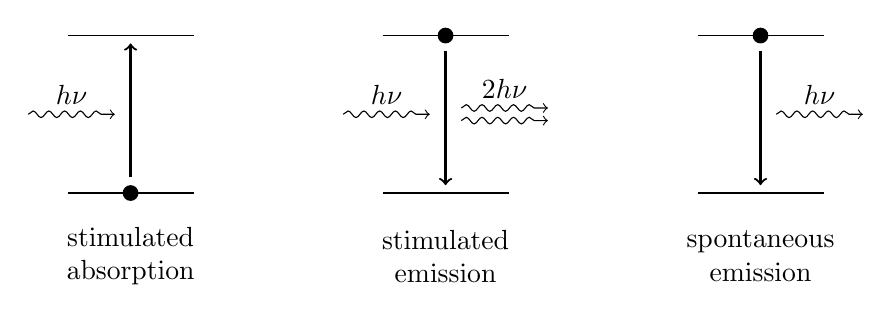
\begin{tikzpicture}[decoration = {snake,post length=3pt,amplitude=1.2pt,segment length=2mm}]
            \draw (0,0)--(1.6,0);
            \draw (0,2)--(1.6,2);
            \fill[black] (0.8,0) circle (0.1);
            \draw[->,thick] (0.8,0.2)--(0.8,1.9);
            \draw[->,decorate] (-0.5,1)--node[above]{\(h \nu\)}(0.6,1);
            \node[align=center] at (0.8,-0.8){stimulated \\ absorption};
            \draw (4,0)--(5.6,0);
            \draw (4,2)--(5.6,2);
            \fill[black] (4.8,2) circle (0.1);
            \draw[->,thick] (4.8,1.8)--(4.8,0.1);
            \draw[->,decorate] (3.5,1)--node[above]{\(h \nu\)}(4.6,1);
            \draw[->,decorate] (5.0,1.08)--node[above]{\(2 h \nu\)}(6.1,1.08);
            \draw[->,decorate] (5.0,0.92)--(6.1,0.92);
            \node[align=center] at (4.8,-0.8){stimulated \\ emission};
            \draw (8,0)--(9.6,0);
            \draw (8,2)--(9.6,2);
            \fill[black] (8.8,2) circle (0.1);
            \draw[->,thick] (8.8,1.8)--(8.8,0.1);
            \draw[->,decorate] (9.0,1)--node[above]{\(h \nu\)}(10.1,1);
            \node[align=center] at (8.8,-0.8){spontaneous \\ emission};
        \end{tikzpicture}
    \end{figure}
    \begin{enumerate}[topsep=0pt,label=(\roman*)]
        \item \textit{Stimulated absorption}: a photon is absorbed, and the system moves from a lower to an upper level.
        
        Examples: IR/UV-Vis spectroscopy.
        \item \textit{Stimulated emission}: one photon triggers the generation of another, and the system moves from an upper to a lower level.
        
        Example: LASER.
        \item \textit{Spontaneous emission}: not triggered by a photon, and the system moves from an upper to a lower level.
        
        Examples: flame test, emission lamp, LED.
    \end{enumerate}

    These three processes all involve the molecule (or atom) moving from one energy level to another, and thus leading to a change in the populations of the levels. Therefore, like other processes, we can sensibly talk about the rate at which these populations change. The rates of these three processes are influenced by different factors and so, depending on the circumstances, one may dominate over the other.

    \subsubsection{The Einstein Coefficients}
    Consider transitions involving the two levels \(\ket{i}\) and \(\ket{j}\). Let their populations be \(n_i\) and \(n_j\), respectively, and let the energy separation between the levels be \(\Delta E=h\nu\). For the moment we will assume that both levels are non-degenerate, i.e. \(g_i=g_j=1\).

    \begin{figure}
        \centering
        \begin{tikzpicture}
            \draw (0,0)node[left]{\(n_i\)}--(1.5,0)node[right]{\(\ket{i}\)};
            \draw (0,1.8)node[left]{\(n_j\)}--(1.5,1.8)node[right]{\(\ket{j}\)};
        \end{tikzpicture}
        \caption{A two level system.}
    \end{figure}

    The rate of stimulated absorption can be expressed in terms of the resulting change in the population of the lower level:
    \begin{equation}
        \text{stimulated absorption:}\quad\dv{n_i}{t}=-B_{ij} \rho(\nu) n_i\,,
    \end{equation}
    where \(B_{ij}\) is the \textit{Einstein \(B\) coefficient} for the transition and \(\rho(\nu)\) is the energy density of the radiation at frequency \(\nu\). The Einstein \(B\) coefficient is analogous to the second order rate constant for a chemical reaction, and it has the units \(\!\unit{m}^3\unit{J}^{-1}\unit{s}^{-2}=\!\unit{m}\unit{kg}^{-1}\). \(\rho(\nu)\d{\nu}\) is the energy of photons between \(\nu\) and \(\nu+\d{\nu}\) per unit volume, which can be thought of as the ``concentration of photons'', having units of \(\!\unit{J}\unit{m}^{-3}\), so \(\rho(\nu)\) itself has units \(\!\unit{J}\unit{s}\unit{m}^{-3}\).

    Similarly, the rate of stimulated emission can be expressed in terms of the resulting change in the upper level:
    \begin{equation}
        \text{stimulated emission:}\quad\dv{n_j}{t}=-B_{ji} \rho(\nu) n_j\,.
    \end{equation}

    It can be shown that the Einstein coefficients for these two processes are related by \(g_i B_{ij}=g_j B_{ji}\), where \(g_i\) and \(g_j\) are the degeneracies of the levels \(i\) and \(j\), respectively. For the present discussion we assumed both levels to be non-degenerate, so \(B_{ij}=B_{ji}\). The values of these coefficients are then given by
    \begin{equation}
        B_{ij}=\frac{8 \pi^3}{(4\pi\epsilon_0) 3 h^2} \abs{R_{ij}}^2\,,
    \end{equation}
    where \(\epsilon_0\) is the permittivity of free space. \(R_{ij}\) is the \textit{transition moment} given by
    \begin{equation}
        R_{ij} \coloneqq \mel{j}{\hat{\mu}}{i} \equiv \int\dd{\tau} \psi_j^* \hat{\mu} \psi_i\,,
    \end{equation}
    in which \(\psi_i\) and \(\psi_j\) are the wavefunctions of the two states, and \(\hat{\mu}\) is the \textit{electric dipole moment operator}.\footnote{All these results stated above come from time-dependent perturbation theory. See C7: Further Quantum Mechanics or Principles of Quantum Mechanics for details.}

    Often we can say whether a transition moment is zero or not just by directly inspecting the symmetry of the integrand --- this results in the selection rules which you have already come across. A \textit{forbidden transition} has \(R_{ij}=0\), so there is no absorption or emission of radiation, and an \textit{allowed transition} has \(R_{ij}\ne 0\) so transitions can take place.

    The rate of spontaneous emission can be written as
    \begin{equation}\label{spontaneous_emission}
        \text{spontaneous emission:}\quad \dv{n_j}{t}=-A_{ij} n_j\,,
    \end{equation}
    where \(A_{ij}\) is the Einstein \(A\) coefficient. The radiation density is not involved in this expression as no photon is needed to trigger spontaneous emission. Hence, \(A_{ij}\) is analogous to a first order rate constant, with unit \(\mathrm{s}^{-1}\).

    \subsubsection{Why Spontaneous Emission}
    A question is: why does spontaneous emission occur at all? This is a tough question. We need quantum field theory to fully answer it. Instead, we will do a thought experiment to imagine what will happen without it.

    Consider a body of interest surrounded by a large black body radiator being held at constant temperature \(T_{\text{surr}}\), but they are separated by vacuum.

    \begin{figure}[ht!]
        \centering
        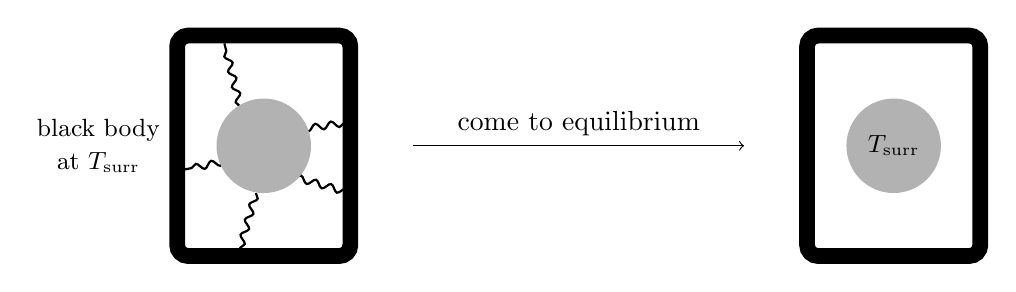
\begin{tikzpicture}[decoration = {snake,amplitude=1.2pt,segment length=2mm}]
            \draw[rounded corners, line width=2mm] (0,0) rectangle (2.2,2.8); 
            \node[align=center] at (-1,1.4){\small black body \\ \small at \(T_{\text{surr}}\)};
            \draw[decorate,thick] (0.8,1.9)--(0.6,2.7);
            \draw[decorate,thick] (1.5,1)--(2.2,0.8);
            \draw[decorate,thick] (1.5,1.6)--(2.2,1.7);
            \draw[decorate,thick] (1,0.8)--(0.8,0.1);
            \draw[decorate,thick] (0.6,1.2)--(0.1,1.1);
            \fill[gray!60] (1.1,1.4) circle (0.6);
            \draw[->] (3,1.4)--node[above]{come to equilibrium}(7.2,1.4);
            \draw[rounded corners, line width=2mm] (8,0) rectangle (10.2,2.8); 
            \fill[gray!60] (9.1,1.4) circle (0.6);
            \node at (9.1,1.4) {\small \(T_{\text{surr}}\)};
        \end{tikzpicture}
        \caption{A body of interest held in vacuum, surrounded by a black body of temperature \(T_{\text{surr}}\).}
    \end{figure}

    From our experience, we know that the body will eventually come to the same temperature as the black body i.e. the two objects will come to equilibrium. It will do this by gaining or losing energy by absorbing or emitting photons.

    The temperature of the object is reflected in the way in which particles are distributed amongst the energy levels, as predicted by the Boltzmann distribution. The higher the temperature, the greater the population of the upper levels.

    As a simplification, suppose our object has only two energy levels, \(i\) and \(j\), and suppose there are only stimulated absorption and stimulated emission. The rate of change of the population of level \(i\) is
    \begin{equation}
        \dv{n_i}{t}=\underbrace{-B_{ij}\rho(\nu)n_i}_{\begin{subarray}{c}\text{stimulated} \\ \text{absorption} \end{subarray}}+\underbrace{B_{ji}\rho(\nu)n_j}_{\begin{subarray}{c}\text{stimulated} \\ \text{emission} \end{subarray}}\,.
    \end{equation}
    At equilibrium, the population will cease to change, so the derivative will be zero. Thus
    \begin{equation}
        -B_{ij}\rho(\nu)n_{i,\text{eq}}+B_{ji}\rho(\nu)n_{j,\text{eq}}=0\,.
    \end{equation}
    But we know that \(B_{ij}=B_{ji}\), so it follows that, at equilibrium, \(n_{i,\text{eq}}=n_{j,\text{eq}}\). This is impossible as it predicts the object to have infinite temperature by Boltzmann distribution.

    What this thought experiment shows is that, on its own, stimulated emission and stimulated absorption cannot bring bodies to equilibrium with the surrounding. This is why we need spontaneous emission: this process leads to a reduction in the population of the upper level. We can also see that, as the energy separation between the two levels become greater, the population of the upper level must go down as predicted by Boltzmann distribution. Thus, the rate of spontaneous emission must also increase as the energy separation between levels increases. We will see this in the next section.
    \subsubsection{Relationship between the Einstein Coefficients}
    If spontaneous emission is taken into account, the total rate of change of the population of the lower level in our two-level system is
    \begin{equation}\label{population_derivative}
        \dv{n_i}{t}=-B_{ij}\rho(\nu)n_i+B_{ji}\rho(\nu)n_j+A_{ij}n_j\,.
    \end{equation}
    We can use this expression to find the relationship between the Einstein \(A\) and \(B\) coefficients.

    For a black body at temperature \(T\), the radiation density is given by the Planck law
    \begin{equation}
        \rho(\nu)\d{\nu}=\frac{8\pi h\nu^3}{c^3}\frac{1}{\exp(h\nu/k_B T)-1}\dd{\nu}\,.
    \end{equation}
    A derivation of this is shown in the appendix \cref{Chap:Black_Body}. The Boltzmann distribution predicts that, at equilibrium, the populations of the levels \(i\) and \(j\) will be
    \begin{equation}
        n_{i,\text{eq}}=\frac{N}{q}\exp\left(-\frac{\epsilon_i}{k_BT}\right)\quad \text{and}\quad n_{j,\text{eq}}=\frac{N}{q}\exp\left(-\frac{\epsilon_j}{k_BT}\right)\,,
    \end{equation}
    where \(\epsilon_i\) and \(\epsilon_j\) are the energies of the two levels. The ratio of populations is therefore
    \begin{equation}
        \frac{n_{j,\text{eq}}}{n_{i,\text{eq}}}=\exp\left(-\frac{\Delta\epsilon}{k_B T}\right)\,,
    \end{equation}
    where \(\Delta\epsilon=\epsilon_j-\epsilon_i\) is the energy gap.

    At equilibrium the time derivative of population (\ref{population_derivative}) is zero. If we substitute Planck's law and population ratio into the equation and recognize \(\Delta\epsilon=h\nu\), then we find
    \begin{equation}
        A_{ji}=\frac{8\pi h\nu^3}{c^3}B_{ji}\,.
    \end{equation}

    Two remarks:
    \begin{enumerate}[topsep=0pt,label=(\roman*)]
        \item the Einstein \(A\) and \(B\) coefficients are related; and
        \item the rate of spontaneous emission increases dramatically with frequency \(\sim \nu^3\).
    \end{enumerate}

    Under typical conditions, spontaneous emission in the microwave is slower than competing processes, whereas in UV/Vis spontaneous emission is dominant.

    \subsection{Linewidths}
    Although we refer to peaks as ``lines'' in spectra, in fact the absorptions we see are not at precisely defined frequencies; rather, there is always a spread of frequencies over which the absorption is seen. If we plot the absorbance against frequency, we typically observe a bell-shaped curve. It is usual to specify the width of this line by its \textit{width at half maximum}, \(\Delta\nu\).
    \begin{figure}[ht!]
        \centering
        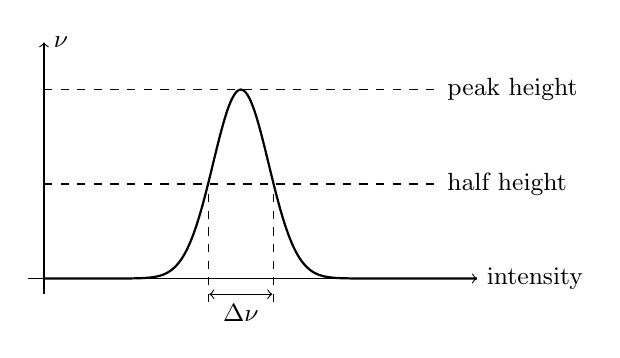
\begin{tikzpicture}
            \draw[->] (-0.2,0)--(5.5,0)node[right]{\small intensity};
            \draw[->] (0,-0.2)--(0,3)node[right]{\small\(\nu\)};
            \draw[dashed] (0,2.4)--(5,2.4)node[right]{\small peak height};
            \draw[dashed] (0,1.2)--(5,1.2)node[right]{\small half height};
            \draw[thick,domain=-2.5:3, smooth, variable=\x,samples=100] plot ({\x+2.5}, {2.4*2.72^(-4*\x*\x)});
            \draw[dashed] (2.09,-0.3)--(2.09,1.2);
            \draw[dashed] (2.91,-0.3)--(2.91,1.2);
            \draw[<->] (2.1,-0.2)--node[below]{\small\(\Delta\nu\)}(2.9,-0.2);
        \end{tikzpicture}
        \caption{The linewidth is defined as the width for which a peak has a height equal to a half of its maximum.}
    \end{figure}

    Sometimes the linewidth is limited by the spectrometer being used, but it is often found that the improvements in the spectrometer eventually lead to no further reduction in the linewidth. It is then assumed that the linewidth seen is a fundamental property of the sample itself.

    There are a number of different effects which are responsible for the finite width of lines in the spectrum. Understanding these is important as, if the source of the linewidth is identified, it may be possible to alter the experimental conditions so as to reduce the linewidth and hence improve the resolution.

    The first two types of line broadening we will consider are both associated with the fact that the molecules spend a finite amount of time in any particular energy level. Molecules are constantly moving from one energy level to another, which may occur because of the collisions between molecules, or due to the molecules emitting a photon and so dropping down to a lower level. Whatever mechanism by which the molecule moves from one energy level to another, we can characterise the process by saying that a particular energy level has a certain \textit{lifetime} \(\tau\). In quantum mechanics, a finite lifetime implies an uncertainty in the energy of states --- this is the \textit{generalised principle of uncertainty}, which states that
    \begin{equation}\label{energy_uncertainty}
        \tau\Delta E\approx\hbar\,.
    \end{equation}

    We see that a shorter-lived state has greater uncertainty in its energy than a longer lived state. This uncertainty in the energy translates to a non-zero linewidth, as a range of frequencies can now cause the transition. \Cref{energy_uncertainty} can be re-expressed in frequency as
    \begin{equation}\label{line_width_life_time}
        \Delta\nu=\frac{1}{2\pi\tau}\,,
    \end{equation}
    where \(\Delta\nu\) is the uncertainty in the frequency of the line, which we identified as the linewidth.

    \begin{figure}[ht!]
        \centering
        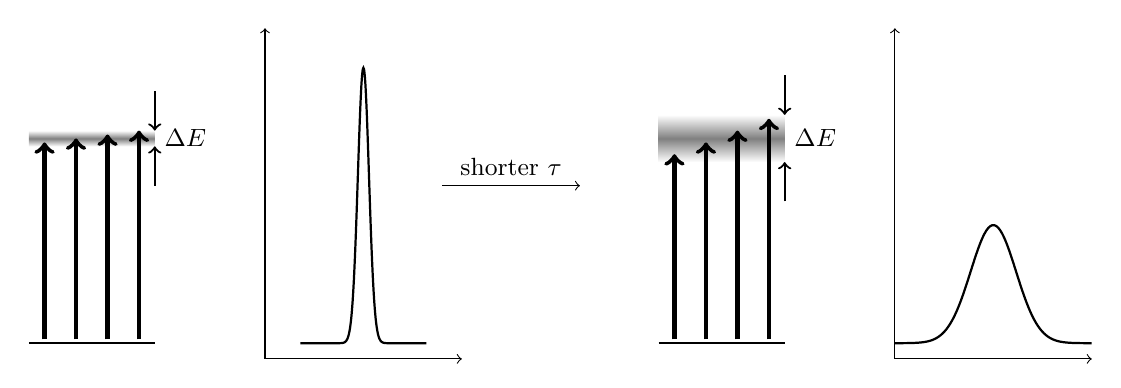
\begin{tikzpicture}
            \draw[thick] (0,0)--(1.6,0);
            \fill[top color=white,bottom color=white,middle color=gray]  (0,2.5) rectangle (1.6,2.7);
            \draw[->,thick] (1.6,2)--(1.6,2.5);
            \draw[->,thick] (1.6,3.2)--(1.6,2.7);
            \node at (1.6,2.6)[right]{\small \(\Delta E\)};
            \foreach \i in {0,...,3}{
                \draw[->,ultra thick] (0.2+\i*0.4,0.05)--(0.2+\i*0.4,2.55+0.05*\i);
            }
            \draw[->] (3,-0.2)--(5.5,-0.2);
            \draw[->] (3,-0.2)--(3,4);
            \draw[thick,domain=-0.8:0.8, smooth, variable=\x,samples=100] plot ({\x+4.25}, {3.5*2.72^(-100*\x*\x)});

            \draw[->] (5.25,2)--node[above]{\small shorter \(\tau\)}(7,2);

            \draw[thick] (8,0)--(9.6,0);
            \fill[top color=white,bottom color=white,middle color=gray]  (8,2.3) rectangle (9.6,2.9);
            \draw[->,thick] (9.6,1.8)--(9.6,2.3);
            \draw[->,thick] (9.6,3.4)--(9.6,2.9);
            \node at (9.6,2.6)[right]{\small \(\Delta E\)};
            \foreach \i in {0,...,3}{
                \draw[->,ultra thick] (8.2+\i*0.4,0.05)--(8.2+\i*0.4,2.4+0.15*\i);
            }
            \draw[->] (11,-0.2)--(13.5,-0.2);
            \draw[->] (11,-0.2)--(11,4);
            \draw[thick,domain=-1.25:1.25, smooth, variable=\x,samples=100] plot ({\x+12.25}, {1.5*2.72^(-6*\x*\x)});
        \end{tikzpicture}
    \end{figure}

    \subsubsection{Natural Line Broadening}
    If a molecule or atom is in anything other than the ground state, it is possible for spontaneous emission to take place, the rate of which is given by (\ref{spontaneous_emission}) in terms of the Einstein \(A\) coefficient. As a result of this, the excited state has a finite lifetime, leading to line broadening.

    We see from \cref{spontaneous_emission} that spontaneous emission is a first-order process so, just as in chemical kinetics, we can use the concept of a half-life to describe its rate. In chemical kinetics the half-life is \(\ln 2/k_{1\text{st}}\) but it is more usual in spectroscopy to define a natural lifetime, \(\tau_{\text{e}}\), according to
    \begin{equation}
        \tau_{\text{e}}=\frac{1}{A_{ij}}\,.
    \end{equation}
    The linewidth due to this process is hence
    \begin{equation}
        \Delta\nu=\frac{A_{ij}}{2\pi}\,.
    \end{equation}

    This effect is referred to as \textit{natural line broadening} because it arises from the fundamental lifetime of the state imposed by the spontaneous emission rate. This is always unavoidable.

    Here are some typical values to help you get some sense of it:
    \begin{enumerate}[topsep=0pt,label=(\roman*)]
        \item Electronic excited state: \(\tau_{\text{e}}\approx 10\unit{ns}\) gives \(\Delta\nu=5\times 10^{-4}\unit{cm}^{-1}\) or \(16\unit{MHz}\).
        \item Rotational excited state: rate is much slower, and typically get \(\Delta\nu\sim 10^{-4}\unit{Hz}\).
    \end{enumerate}
    \subsubsection{Pressure (Collision) Broadening}
    Collisions between molecules can result in a change of energy level (translational motion readily accommodates any deficit or excess of energy) and so the lifetime of a state is determined by the rate of collisions. If we assume that each collision leads to a change in energy level, then the lifetime, \(\tau\), is the mean time between collisions. The resulting line broadening can then be estimated using (\ref{line_width_life_time}).

    The mean time between collisions can be estimated using gas kinetic theory: the collision rate depends on the size of the molecules (the collision cross-section \(\sigma\)), the temperature and the pressure. As the pressure goes up, the rate of collision increases and so the mean time between collisions (which we identified as the lifetime) decreases. The linewidth is therefore proportional to the pressure, and hence the name of pressure broadening. With a full treatment of kinetic theory (derivation in appendix \cref{Chap:Pressure_broadening}), we can obtain the expression
    \begin{equation}
        \Delta\nu_{\text{press}}=Kp\,,
    \end{equation}
    where
    \begin{equation}
        K=\frac{2\sigma}{\sqrt{k_BT\pi^3 m}}\,.
    \end{equation}

    Pressure broadening tends to be the dominant contribution to the linewidth in microwave spectroscopy and an important contribution for lines in the infra-red.

    \subsubsection{Doppler Broadening}
    Our next source of broadening is unrelated to the lifetime of the states. It originates from the Doppler effect.

    The Doppler shift is familiar to us as the shift in frequency of a siren as a fire engine passes by. Molecules are moving in random directions relative to the radiation which is passing through the sample and at a range of speeds so the effect is to generate a spread of frequencies which are absorbed or emitted by the molecules: this is the origin of the Doppler induced linewidth. Of course, the speed with which molecules move is only a tiny fraction of the speed of light, so the frequency shifts are very small compared to the absolute frequency, but nevertheless can be a significant contribution to the linewidth.

    \begin{figure}[ht!]
        \centering
        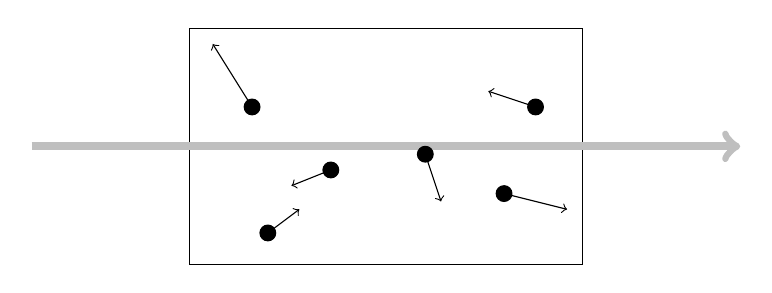
\begin{tikzpicture}
            \draw (0,0) rectangle (5,3);
            \draw[gray!50,line width = 0.1 cm,->] (-2,1.5)--(7,1.5);
            \draw[fill=black] (1,0.4) circle (0.1);
            \draw[->] (1,0.4)--(1.4,0.7);
            \draw[fill=black] (0.8,2) circle (0.1);
            \draw[->] (0.8,2)--(0.3,2.8);
            \draw[fill=black] (1.8,1.2) circle (0.1);
            \draw[->] (1.8,1.2)--(1.3,1);
            \draw[fill=black] (3,1.4) circle (0.1);
            \draw[->] (3,1.4)--(3.2,0.8);
            \draw[fill=black] (4.4,2) circle (0.1);
            \draw[->] (4.4,2)--(3.8,2.2);
            \draw[fill=black] (4,0.9) circle (0.1);
            \draw[->] (4,0.9)--(4.8,0.7);
        \end{tikzpicture}
    \end{figure}

    Gas kinetic theory can be used to derive an expression for the Doppler broadening linewidth. If a molecule is moving at a non-relativistic speed \(s\) towards a source of radiation of frequency \(\nu_0\), the apparent frequency is shifted to \(\nu_{\text{app}}\), and if the molecule is moving away from the source of apparent frequency is \(\nu_{\text{rec}}\), where
    \begin{equation}\label{doppler_frequency}
        \nu_{\text{app}}=\left(1+\frac{s}{c}\right)\nu_0\,,\; \nu_{\text{rec}}=\left(1-\frac{s}{c}\right)\nu_0\,.
    \end{equation}
    The Maxwell--Boltzmann distribution gives the distribution of speeds which in turn leads to a distribution of frequencies received by the molecules. The required distribution is that in one dimension as the Doppler shift depends on the speed along the direction in which the light is passing. This distribution is
    \begin{equation}
        f(s)=\left(\frac{m}{2\pi k_B T}\right)^{\frac{1}{2}}\ee^{-ms^2/2k_B T}\,,
    \end{equation}
    where \(f(s)\d{s}\) is the fraction of molecules with speeds between \(s\) and \(s+\d{s}\) along the propagation direction of the light. This expression can be converted into a distribution of frequencies by rewriting (\ref{doppler_frequency}) as
    \begin{equation}
        s=\pm\frac{c}{\nu_0}(\nu_{\text{obs}}-\nu_0)\,,
    \end{equation}
    where \(\nu_{\text{obs}}\) includes both the receding and approaching molecules. Hence, we get
    \begin{equation}
        f(\nu_{\text{obs}})=\left(\frac{m}{2\pi k_B T}\right)^{\frac{1}{2}}\exp\left[-\frac{mc^2(\nu_{\text{obs}}-\nu_0)^2}{2k_B T\nu_0^2}\right]\,.
    \end{equation}
    This distribution is a Gaussian function with its maximum at \(\nu_{\text{obs}}=\nu_0\), and drops to a half at
    \begin{equation}
        \nu_{1/2}=\nu_0\pm\frac{\nu_0}{c}\left(\frac{2k_B T\ln 2}{m}\right)^{\frac{1}{2}}\,.
    \end{equation}
    Hence we get the expression of Doppler broadening
    \begin{equation}
        \Delta\nu_{\text{doppler}}=\frac{2\nu_0}{c}\left(\frac{2k_B T\ln 2}{m}\right)^{\frac{1}{2}}\,.
    \end{equation}
    The Doppler broadening is proportional to the frequency: this is in contrast to the pressure broadening which is independent of frequency. Doppler broadening tends to become dominant for transitions in the visible region. At room temperature, Doppler linewidth in IR is \(\sim 10^{-3}\unit{cm}^{-1}\), while in visible region, this increases to \(\sim 0.1\unit{cm}^{-1}\).

    When more than one source of line broadening is present, it is not correct to simply add the different linewidths together to obtain an overall linewidth. Rather, the line shapes due to the different kinds of line broadening must be convoluted with one another: we will often ignore this complication. When one source of line broadening is dominant then the overall linewidth is, to a good approximation, equal to that of the dominant source.
    \subsection{Notations and Conventions}
    Typically in spectroscopy we identify lines as being associated with transitions between energy levels (or states), and we then label the transition according to the quantum numbers which characterise the levels. Selection rules are also expressed in terms of the quantum numbers for the levels involved.
    
    There are conventions about the way in which transitions are labelled and referred to and it is important to adhere to these. Suppose that we are concerned with the transitions between two levels \(\mathrm{A}\) and \(\mathrm{B}\), and that \(\mathrm{A}\) is the lower energy level.

    \begin{enumerate}[topsep=0pt,label=(\roman*)]
        \item A transition between these levels can be signified by an arrow connecting them: the
        lower energy level is always written on the right
        \begin{itemize}[topsep=0pt]
            \item absorption: \(\mathrm{B\leftarrow A}\)
            \item emission: \(\mathrm{B\rightarrow A}\)
        \end{itemize}
        \item Transitions are labelled with the quantum numbers of the lower level.
        \item The change in any quantum number is given as
        \begin{equation}
            (\text{quantum number of upper level})-(\text{quantum number of lower level})\,.
        \end{equation}
        \item Where a distinction is to be made, quantum numbers referring to the lower energy level are denoted with a double prime e.g. \(J''\); quantum numbers referring to the higher energy level are denoted with a single prime e.g. \(J'\).   
    \end{enumerate}
    \subsection{How to Think about Spectroscopy}
    When we record a spectrum, all we end up with is a set of lines whose frequencies and intensities we can measure. What we cannot tell just by looking at the lines is which energy levels are involved in the transition which leads to each line. To find out anything useful from the spectrum, our first step has to be to assign the lines.

    By \textit{assign} we usually mean specifying the quantum numbers of the energy levels involved. There may be more than one quantum number needed to specify the level, depending on the complexity of the problem.

    The way we go about assigning and interpreting a spectrum is as follows:
    \begin{enumerate}[topsep=0pt,label=(\roman*)]
        \item We start with a model for the energy levels. Typically, we use the energy levels which are available from solving the Schr\"{o}dinger equation for simple systems such as the rigid rotor or the harmonic oscillator.
        \item We then determine the selection rules which apply to these levels and thus predict the form of the spectrum, taking into account that the intensities will be affected by the populations of the energy levels as predicted by the Boltzmann distribution.
        \item Having done this, we can compare the predicted spectrum with the real spectrum, and see if they can be made to match up. Typically there will be parameters in our model which can be adjusted, such as rotational constants and vibrational frequencies. The process of matching up the experimental and predicted spectra is often aided by looking for patterns, such as repeated spacings of lines.
        \item If there is reasonable agreement between the two spectra, then the assignment process is complete as we know the assignment for the predicted spectrum. The values of any parameters needed can then be interpreted, for example to obtain bond lengths.
        \item However, the match between the experimental and predicted spectra is rarely perfect. Usually we need to refine our model used for the energy levels in order to obtain a better fit --- for example by introducing the effects of anharmonicity or centrifugal distortion.
    \end{enumerate}

    The process of assigning and understanding a spectrum is thus one of refining the model in order to obtain the best agreement. Recording the spectrum with higher precision or resolution will often reveal further features which require more refinement of the model.

    \newpage
    \section{Rotational Spectroscopy}
    As we have already seen before, there are a set of energy levels associated with the overall rotation of molecules; transitions between these levels give rise to spectra which typically appear in the microwave part of the spectrum. Such spectra are called \textit{microwave} or \textit{pure rotational spectra}.

    In this section we will extend the discussion to include non-linear molecules and also look at some additional effects, such as centrifugal distortion and the influence of electric fields.

    \subsection{Classification of Rotating Molecules}
    For the purposes of this discussion we consider a molecule to be a rigid body in which the atoms occupy fixed positions relative to one another, and in which the nuclei have negligible size.

    The \textit{moment of inertia} of a molecule with respect to a particular axis is defined as
    \begin{equation}
        I=\sum_i m_ir_i^2\,,
    \end{equation}
    where \(m_i\) is the mass of the atom \(i\) and \(r_i\) is the perpendicular distance from the atom to the axis.

    We can compute the moment of inertia about any axis, but there will be one such axis which has the greatest moment of inertia: this axis is labeled \(c\) and has moment of inertia \(I_c\). There is another axis, labeled \(a\), which has the minimum moment of inertia \(I_a\), and it can be shown that this axis is perpendicular to the \(c\)-axis. A third axis, labeled \(b\), is perpendicular to the other two. These three axes are called the \textit{principal axes}. The moments of inertia about these principal axes (the principal moments of inertia) are related according to
    \begin{equation}
        I_c\ge I_b\ge I_a\,.
    \end{equation}
    
    This is actually because the moment of inertia of a general object is defined as a symmetric 2-tensor, with components
    \begin{equation}
        I_{ij}=\int\dd{V}\rho(\vb{x})(x_kx_k\delta_{ij}-x_ix_j)\,.
    \end{equation}
    A real symmetric 2-tensor (matrix) can always be diagonalised by an orthogonal matrix (a change of basis), with eigenvalues we denote as \(I_a\), \(I_b\) and \(I_c\), and eigenvectors along the direction of the corresponding principal axes.

    Molecules can be classified according to the relationships of the magnitudes between the principal moments of inertia.

    \subsubsection{Spherical Tops}
    Spherical tops have all three moments of inertia equal. For this to be the case, the molecule must have a high symmetry. In terms of group theory, the three rotations \((R_x, R_y, R_z)\) must transform together as a three-dimensional (triply degenerate) irreducible representation. Those molecules have no dipole moments, so they do not show pure rotational (microwave) spectra. Examples include \(\mathrm{CH_4}\ (T_d)\) and \(\mathrm{SF_6}\ (O_h)\).
    \subsubsection{Symmetric Top}
    Symmetric tops have two of the moments of inertia equal and the third different from the other two.
    \begin{figure}[ht!]
        \centering
        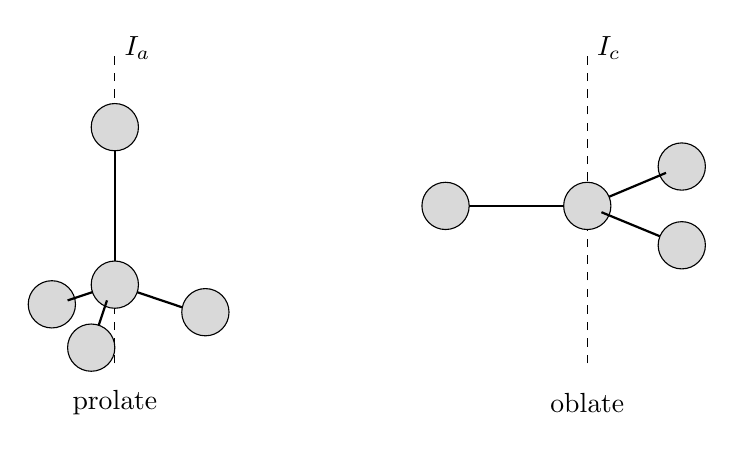
\begin{tikzpicture}
            \draw[dashed] (0,0)--(0,4)node[right]{\(I_a\)};
            \draw[fill=gray!30] (-0.8,0.75) circle (0.3);
            \draw[thick] (0,1)--(-0.6,0.8);
            \draw[thick] (0,1.3)--(0,2.7);
            \draw[thick] (0,1)--(0.95,0.68);
            \draw[fill=gray!30] (0,1) circle (0.3);
            \draw[fill=gray!30] (0,3) circle (0.3);
            \draw[thick] (-0.1,0.8)--(-0.3,0.2);
            \draw[fill=gray!30] (-0.3,0.2) circle (0.3);
            \draw[fill=gray!30] (1.15,0.65) circle (0.3);
            \node at (0,-0.5) {prolate};
            \draw[dashed] (6,0)--(6,4)node[right]{\(I_c\)};
            \draw[fill=gray!30] (7.2,2.5) circle (0.3);
            \draw[thick] (6,2)--(7,2.42);
            \draw[fill=gray!30] (6,2) circle (0.3);
            \draw[thick] (6.18,1.92)--(7.2,1.5);
            \draw[fill=gray!30] (4.2,2) circle (0.3);
            \draw[fill=gray!30] (7.2,1.5) circle (0.3);
            \draw[thick] (4.5,2)--(5.7,2);
            \node at (6,-0.5) {oblate};
        \end{tikzpicture}
    \end{figure}

    If the two moments of inertia which are equal are larger than the third moment of inertia, the molecule is termed a \textit{prolate symmetric top}:
    \begin{equation}
        I_c=I_b>I_a\,.
    \end{equation}
    An example is \(\mathrm{CH_3Cl}\).

    If the two moments of inertia which are equal are smaller than the third moment of inertia, the molecule is termed an \textit{oblate symmetric top}:
    \begin{equation}
        I_c>I_b=I_a\,.
    \end{equation}
    An example is \(\mathrm{BF_3}\).

    It is evident that symmetric tops must have a certain minimum of symmetry such that two of the rotations e.g. \((R_x,R_y)\) transform together as a two-dimensional irreducible representation. It can be shown that this requirement is satisfied by molecules possessing a single \(C_n\) axis, with \(n>2\), or an \(S_4\) axis. This symmetry test is by far the easiest way of deciding whether or not a molecule is a symmetric top.
    \subsubsection{Asymmetric Tops}
    In an asymmetric top, all three moments of inertia are different. Each of \(R_x\), \(R_y\) and \(R_z\) transforms as one-dimensional irreducible representations.

    \subsubsection{Linear Molecules}
    \begin{figure}[ht!]
        \centering
        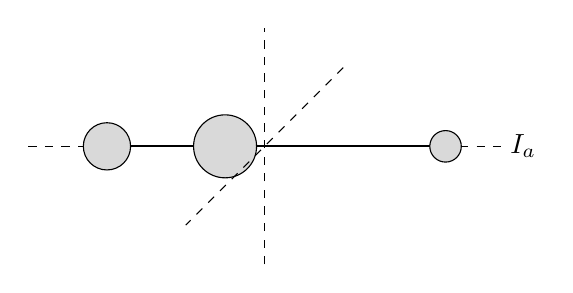
\begin{tikzpicture}
            \draw[dashed] (-3,0)--(3,0)node[right]{\(I_a\)};
            \draw[thick] (-2,0)--(2.3,0);
            \draw[fill=gray!30] (-0.5,0) circle (0.4);
            \draw[fill=gray!30] (-2,0) circle (0.3);
            \draw[fill=gray!30] (2.3,0) circle (0.2);
            \draw[dashed] (0,-1.5)--(0,1.5);
            \draw[dashed] (1,1)--(-1,-1);
        \end{tikzpicture}
    \end{figure}
    If we consider the atoms to be point masses, then the moment of inertia about the internuclear axis of a linear molecule is zero; the other two moments of inertia, about axes perpendicular to the internuclear axis, are equal. Thus, a linear molecule is a special case of a prolate symmetric top with \(I_a=0\).

    \subsection{Rotational Energy Levels}
    The general Hamiltonian for rotation can be written as
    \begin{equation}
        H=\frac{1}{2}\left(\frac{J_a^2}{I_a}+\frac{J_b^2}{I_b}+\frac{J_c^2}{I_c}\right)\,.
    \end{equation}
    The expression of the energy levels vary as the relation between \(I_a\), \(I_b\) and \(I_c\) changes in different tops.
    \subsubsection{Symmetric Tops}
    \subsubsection*{Prolate Tops}
    A prolate symmetric top has \(I_c=I_b>I_a\), so we can factorise the Hamiltonian as
    \begin{equation}
        H=\frac{1}{2}\left[\frac{\vb{J}^2}{I_b}+J_a^2\left(\frac{1}{I_a}-\frac{1}{I_b}\right)\right]\,.
    \end{equation}
    Then the energy levels of a prolate symmetric top can be easily obtained as
    \begin{equation}
        E_{J,K}=BJ(J+1)+(A-B)K^2\,,
    \end{equation}
    where the quantum numbers have ranges \(J=0,1,2,\dots\) and \(K=-J,-J+1,\dots,J\). These levels are sometimes denoted \(J_K\). \(A\) and \(B\) are the rotational constants associated with the moments of inertia about the \(a\)- and \(b\)-axes, respectively. Their values are given in \(\!\unit{J}\) by
    \begin{equation}
        A=\frac{\hbar^2}{2I_a}\qquad B=\frac{\hbar^2}{2I_b}\,.
    \end{equation}
    Alternatively we can express the energies and rotational constants in wavenumbers:
    \begin{equation}\label{prolate_top_energy}
        \tilde{E}_{J,K}=\tilde{B}J(J+1)+(\tilde{A}-\tilde{B})K^2\,,
    \end{equation}
    where the rotational constants in wavenumbers are
    \begin{equation}
        \tilde{A}=\frac{h}{8\pi^2\tilde{c}I_a}\qquad\tilde{B}=\frac{h}{8\pi^2\tilde{c}I_b}\,.
    \end{equation}

    As we have seen before, the quantum number \(J\) gives the magnitude of total angular momentum \(\sqrt{J(J+1)}\hbar\). The quantum number \(K\) gives the component of the angular momentum along the unique \(a\)-axis, which is \(K\hbar\).

    \begin{figure}[ht!]
        \centering
        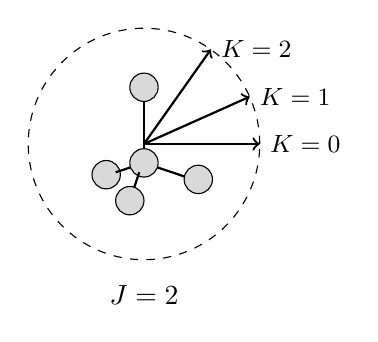
\begin{tikzpicture}[scale=0.6]
            \draw[fill=gray!30] (-0.8,0.75) circle (0.3);
            \draw[thick] (0,1)--(-0.6,0.8);
            \draw[thick] (0,1.3)--(0,2.5);
            \draw[thick] (0,1)--(0.95,0.68);
            \draw[fill=gray!30] (0,1) circle (0.3);
            \draw[fill=gray!30] (0,2.6) circle (0.3);
            \draw[thick] (-0.1,0.8)--(-0.3,0.2);
            \draw[fill=gray!30] (-0.3,0.2) circle (0.3);
            \draw[fill=gray!30] (1.15,0.65) circle (0.3);
            \draw[dashed] (0,1.4) circle (2.45);
            \draw[thick,->] (0,1.4)--(2.45,1.4)node[right]{\small \(K=0\)};
            \draw[thick,->] (0,1.4)--(2.237,2.4)node[right]{\small \(K=1\)};
            \draw[thick,->] (0,1.4)--(1.415,3.4)node[right]{\small \(K=2\)};
            \node at (0,-1.8) {\(J=2\)};
        \end{tikzpicture}
    \end{figure}

    The diagram shows the direction of angular momentum (which is also the rotation axis) of a symmetric top at \(J=2\) and \(K=0,1,2\) states.
    \subsubsection*{Oblate Top}
    For an oblate top, we have \(I_c>I_b=I_a\), so we factorise the Hamiltonian as
    \begin{equation}
        H=\frac{1}{2}\left[\frac{\vb{J}^2}{I_b}+J_c^2\left(\frac{1}{I_c}-\frac{1}{I_b}\right)\right]\,.
    \end{equation}
    The rotational energy levels are therefore
    \begin{equation}
        E_{J,K}=BJ(J+1)+(C-B)K^2\,,
    \end{equation}
    where as before, \(J=0,1,\dots\) is the quantum number for the total angular momentum and \(K=-J,\dots,J\) is the quantum number for the component of the angular momentum along the unique axis (\(c\)-axis). \(C\) is the rotational constant associated with the \(c\)-axis
    \begin{equation}
        C=\frac{\hbar^2}{2I_c}\,.
    \end{equation}
    As before, we can also express everything in terms of wavenumbers as well
    \begin{equation}
        \tilde{E}_{J,K}=\tilde{B}J(J+1)+(\tilde{C}-\tilde{B})K^2\,,
    \end{equation}
    where
    \begin{equation}
        \tilde{C}=\frac{h}{8\pi^2\tilde{c}I_c}\,.
    \end{equation}

    \begin{figure}
        \centering
        \begin{tikzpicture}[scale=1.05,y={(0cm,1.2cm)}]
            \draw[->] (0,0)--(0,6.5)node[left]{\small\(\tilde{E}\,/\unit{cm}^{-1}\)};
            \foreach \i in {0,5,10,15,20,25,30}{
                \draw (0,0.2*\i)node[left]{\small\(\i\)}--(0.05,0.2*\i);
            }
            \draw (0.5,0)--(1.5,0)node[right]{\footnotesize\(0\)};
            \draw (0.5,0.1)--(1.5,0.1)node[right=0.5em]{\footnotesize\(1\)};
            \foreach \i in {2,...,5}{
                \draw (0.5,0.05*\i*\i+0.05*\i)--(1.5,0.05*\i*\i+0.05*\i)node[right]{\footnotesize\(\i\)};
            }
            \node at (1,-0.5) {\(K=0\)};
            \foreach \i in {1,...,5}{
                \draw (2.3,0.05*\i*\i+0.05*\i+0.972)--(3.3,0.05*\i*\i+0.05*\i+0.972)node[right]{\footnotesize\(\i\)};
            }
            \node at (2.8,-0.5) {\(K=\pm 1\)};
            \foreach \i in {2,...,5}{
                \draw (4.1,0.05*\i*\i+0.05*\i+3.888)--(5.1,0.05*\i*\i+0.05*\i+3.888)node[right]{\footnotesize\(\i\)};
            }
            \node at (4.6,-0.5) {\(K=\pm 2\)};
            \node at (1.7,1.9) {\small\(J\)};
            \node at (3.5,2.9) {\small\(J\)};
            \node at (5.3,5.8) {\small\(J\)};
            \node at (3,7.2) {(a) prolate};

            \draw[->] (7.5,0)--(7.5,6.5)node[left]{\small\(\tilde{E}\,/\unit{cm}^{-1}\)};
            \foreach \i in {0,50,100,150,200,250,300}{
                \draw (7.5,0.02*\i)node[left]{\small\(\i\)}--(7.55,0.02*\i);
            }
            \foreach \i in {0,...,5}{
                \draw (8,0.2*\i*\i+0.2*\i)--(9,0.2*\i*\i+0.2*\i)node[right]{\footnotesize\(\i\)};
            }
            \node at (8.5,-0.5) {\small \(K=0\)};
            \foreach \i in {1,...,5}{
                \draw (9.8,0.2*\i*\i+0.2*\i-0.071)--(10.8,0.2*\i*\i+0.2*\i-0.071)node[right]{\footnotesize\(\i\)};
            }
            \node at (10.3,-0.5) {\small \(K=\pm 1\)};
            \foreach \i in {2,...,5}{
                \draw (11.6,0.2*\i*\i+0.2*\i-0.284)--(12.6,0.2*\i*\i+0.2*\i-0.284)node[right]{\footnotesize\(\i\)};
            }
            \node at (12.1,-0.5) {\small \(K=\pm 2\)};
            \node at (9.2,6.4) {\small\(J\)};
            \node at (11,6.3) {\small\(J\)};
            \node at (12.8,6.1) {\small\(J\)};
            \node at (10.5,7.2) {(b) oblate};
        \end{tikzpicture}
        \caption{The energy levels of (a) \(\mathrm{CH_3I}\) with \(\tilde{A}=5.11\unit{cm}^{-1}\), \(\tilde{B}=0.250\unit{cm}^{-1}\) and (b) \(\mathrm{NH_3}\) with \(\tilde{C}=6.449\unit{cm}^{-1}\), \(\tilde{B}=10.001\unit{cm}^{-1}\). Each sequence of energy level with the same value of \(K\) is known as a \textit{\(K\) stack}.}
    \end{figure}

    \subsubsection{Linear Molecules}
    As we noted before, linear molecules are a special case of a prolate symmetric top with \(I_a\lll I_b,I_c\). The corresponding rotational constant, \(A\), is thus essentially infinite and so we see from the prolate top energy (\ref{prolate_top_energy}) that only those levels with \(K=0\) need be considered as for higher values of \(K\) the energy would be too high. Recall that the quantum
    number \(K\) gives the angular momentum about the \(a\)-axis, so \(K=0\) means that there is no rotation about this axis (which is the internuclear axis).

    The energy levels of a linear molecule are thus
    \begin{equation}
        E_J=BJ(J+1)\,,
    \end{equation}
    where \(J=0,1,2,\dots\). This is what we are familiar with from Part IB \textit{Introduction to Quantum Mechanics}.
    \subsubsection{Spherical Tops}
    The spherical top has \(I_a=I_b=I_c\), so the Hamiltonian reduces very nicely into
    \begin{equation}
        H=\frac{\vb{J}^2}{2I}\,,
    \end{equation}
    where \(I\) is the moment of inertial about any axis through the centre of mass of the molecule. This results in the same form of energy expression as linear molecules.
    \subsubsection{Asymmetric Tops}
    The energy levels of asymmetric tops do not conform to any simple analytical expression such as those above for linear molecules or symmetric tops. This does not mean that their energy levels cannot be calculated, but it is a tedious process involving matrix diagonalisation for each value of \(J\). However, some molecules can be described as ``near prolate top'' or ``near oblate tops'' and approximate solutions obtained by expanding the asymmetric wavefunction in a basis formed from symmetric tops functions. However, it is now more common to compute them exactly as required and a range of programs exist for this purpose.

    \subsection{Selection Rules and Spectra}
    In order to predict which transitions are allowed, we need to know the selection rules which apply to these energy levels. Determining the form of these rules involves the use of advanced concepts in quantum mechanics; we will therefore simply state the rules.

    The gross selection rule is that, for there to be transitions between the rotational levels, the molecule must possess a permanent dipole moment. We can rationalize this by noting that it is the electric vector of the electromagnetic wave which interacts with the molecule. For such an interaction to change the rotational energy, an electric dipole is required as this unsymmetrical charge distribution can interact with the field as the molecule rotates.

    Assuming that there is a permanent dipole, the additional selection rules are
    \begin{equation}
        \Delta J=\pm 1\quad\Delta K=0\,.
    \end{equation}
    The \(\Delta K=0\) selection rule can be understood by noting that the dipole moment (if there is one) must lie along the unique (symmetry) axis; rotation about this axis does not lead to a change in the orientation of the dipole. \(\Delta J=\pm 1\) because a photon carries a unit of angular momentum. For the total angular momentum to be conserved, the angular momentum of the molecule must also change by one unit.

    \subsubsection{Spectra of Symmetric Tops}
    Knowing the selection rule, all we need to do is find the separation of two energy levels between which transitions are allowed to predict the spectrum.

    For a prolate symmetric top, the energies of the lower and upper states are
    \begin{align}
        \tilde{E}_{J'',K}&=\tilde{B}J''(J''+1)+(\tilde{A}-\tilde{B})K^2\\
        \tilde{E}_{J',K}&=\tilde{B}J'(J'+1)+(\tilde{A}-\tilde{B})K^2\,,
    \end{align}
    where the \(K\) is the same because of the \(\Delta K=0\) selection rule. The energy difference between these levels is
    \begin{align}
        \tilde{\nu}(J'')&=\tilde{E}'_{J',K}-\tilde{E}''_{J'',K}\notag\\
        &=\tilde{B}J'(J'+1)-\tilde{B}J''(J''+1)\,.
    \end{align}

    The allowed transitions have \(\Delta J=J'-J''=\pm 1\). For a transition in absorption, \(\Delta J=+1\), giving
    \begin{equation}
        \tilde{\nu}(J'')=2\tilde{B}(J''+1)\,.
    \end{equation}
    The transition peaks hence occur at \(2\tilde{B}\), \(4\tilde{B}\), \(6\tilde{B}\), so the spacings are constantly \(2\tilde{B}\). This is identical to the pattern seen for linear molecules: the similarity comes about because \(\Delta K=0\) for the symmetric top and \(K\) is restricted to zero for linear molecules.

    However, since \(\Delta K=0\), we can only determine \(B\) and \(I_b\) from the spectra. No information about \(A\) or \(I_a\) can be obtained.
    \subsubsection{Spectra of Linear Molecules}
    The case of linear molecules has already been covered in Part IB. In fact, as we have already seen, the spectra are of the same form as for a symmetric top.

    Shown below is the pure rotational spectrum of \(\mathrm{^1H^{35}Cl}\). The regular spacing of the lines is evident; however, closer inspection reveals that the spacing of the lines are actually slowly decreasing --- this is due to centrifugal distortion, which we will consider in detail in later sections.

    \begin{figure}[ht!]
        \centering
        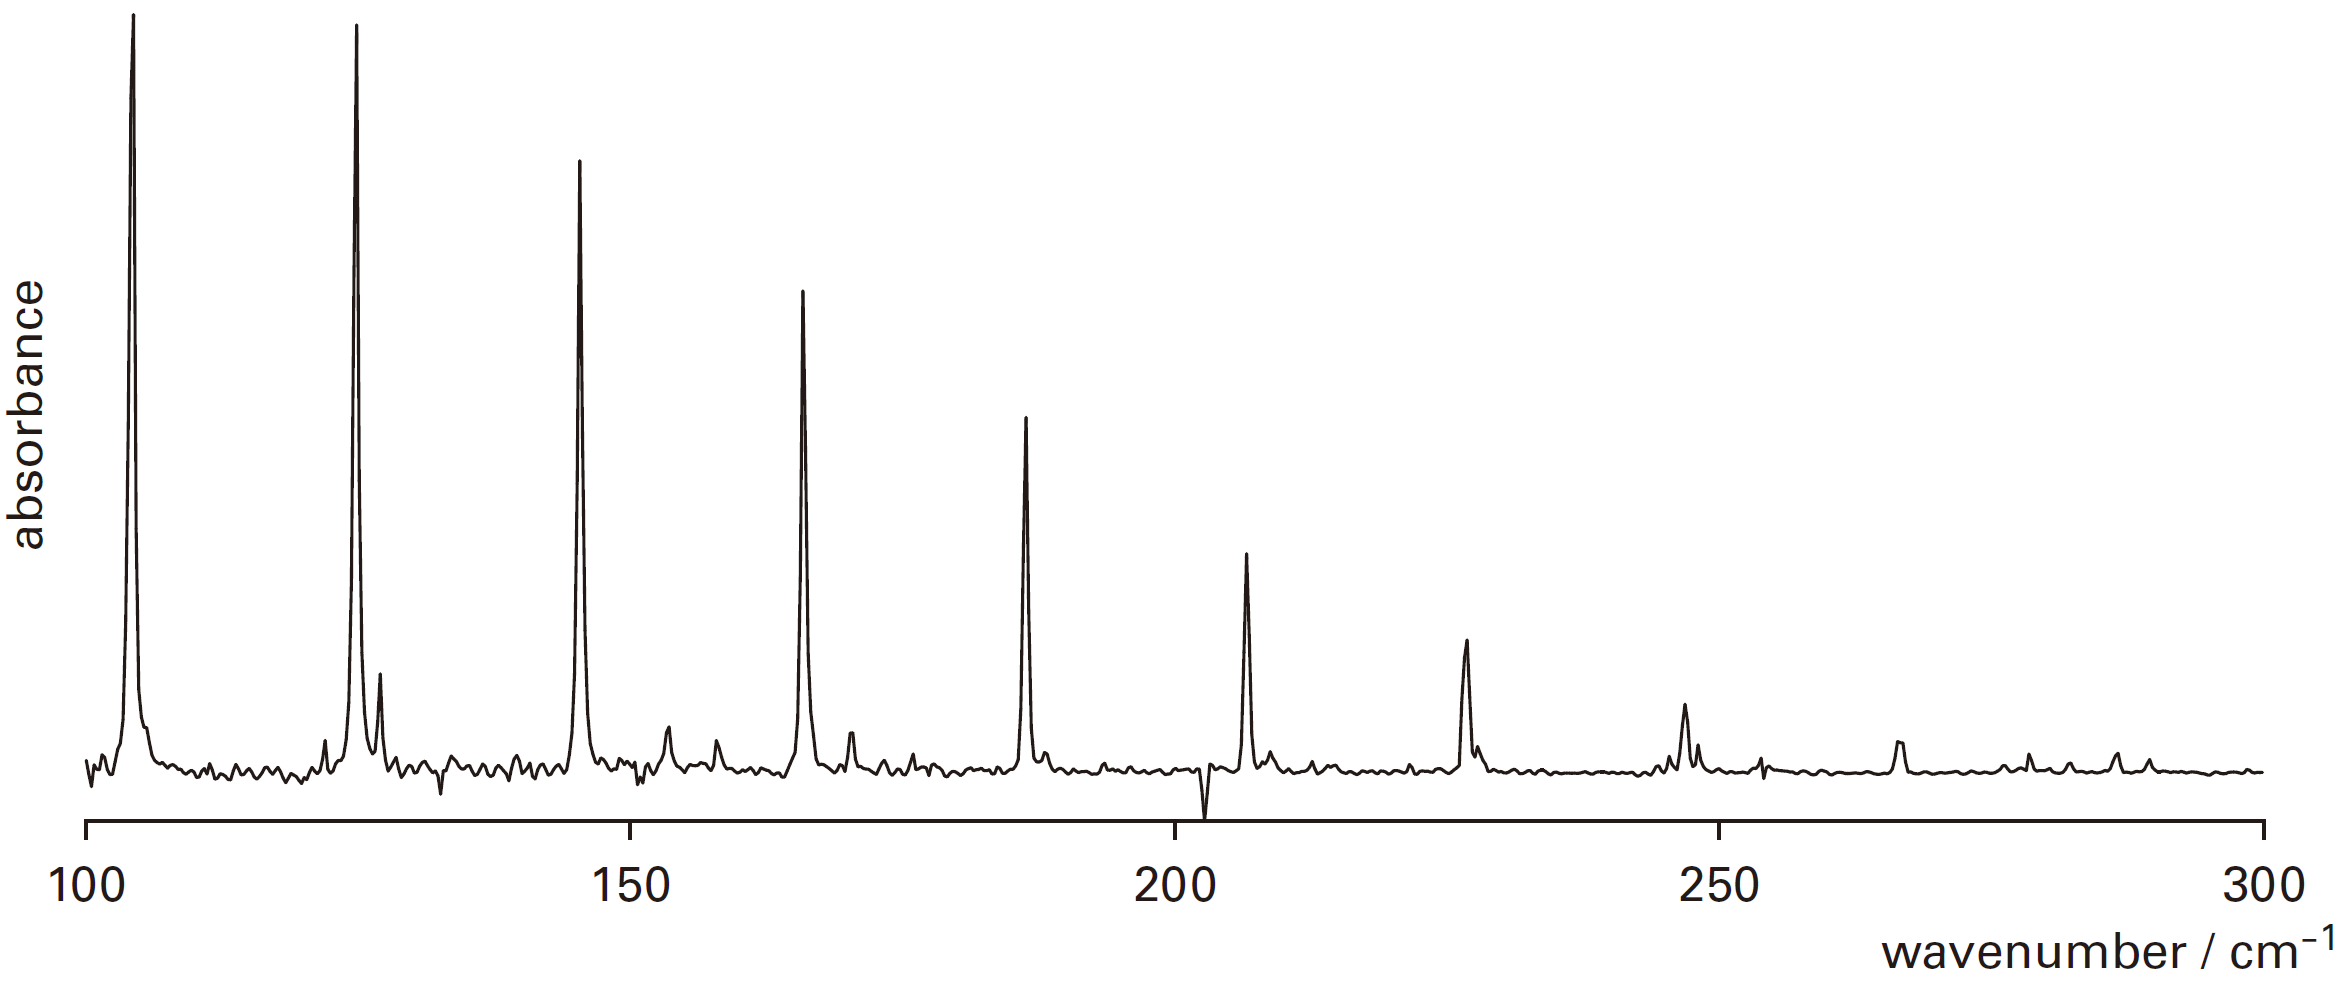
\includegraphics[width=0.8\textwidth]{HCl_microwave.png}
        \caption{Rotational spectroscopy of \(\mathrm{^1H^{35}Cl}\). Figure adapted from official course notes by Prof. Keeler. Spectrum taken by Prof. Wothers.}
    \end{figure}

    \subsubsection{Isotopic Substitution}
    From the spectrum of a symmetric top we can only determine one moment of inertia, so for anything more complex than a diatomic, this is insufficient information to determine all the bond lengths. The spectra of isotopic species give additional moments of inertia which, if it is assumed that the (equilibrium) bond lengths do not change on isotopic substitution, may enable us to find bond lengths.

    For example, in one of the practical experiments, you will record the spectra of \(\mathrm{HCN}\) and \(\mathrm{DCN}\). The resulting two moments of inertia are sufficient to determine both the \(\mathrm{H-C}\) and \(\mathrm{C-N}\) bond lengths.
    \subsection{Intensities}
    The intensity of a transition depends on the details of the three processes by which radiation interacts with the sample. In the IB Molecular Spectroscopy course we assumed that the intensity of an allowed transition was simply proportional to the population of the lower energy level. This is often a good approximation, but in the case of rotational spectroscopy there are further factors which need to be considered in order to understand fully the intensities of the lines.
    \begin{enumerate}[topsep=0pt,label=(\roman*)]
        \item as the molecule rotates faster at higher \(J\) values, the magnitude of the transition dipole moment \(\abs{R_{ij}}\) also increases, leading to higher intensity.
        \item the frequency of the transition affects the net absorption rate (the absorption minus the emission).
    \end{enumerate}

    A derivation is included in \cref{Chap:microwave_intensity} for reference. The result is that the intensity of transition from level \(J\) vary as
    \begin{equation}
        I\propto(J+1)\nu_J^2\exp\left(-\frac{\epsilon_J}{k_B T}\right)\,,
    \end{equation}
    where \(\epsilon_J\) is the energy of the \(J^{\text{th}}\) level, and \(\nu_J\) is the frequency of transition arising from this level (\(\nu_J=2B(J+1)\)). This result is rather a different dependence than one finds by assuming that the intensity is proportional only to the population of the lower energy level.

    \subsection{Centrifugal Distortion}
    So far we have assumed that the rotating molecule is a rigid body, i.e. the bond lengths and angles are unaffected by the rotation of the molecule. Generally, this is a good approximation but in the microwave region measurements can be made with such accuracy that even very small effects due to the lack of rigidity of the molecule can be detected.

    Our expectation is that, as the molecule rotates faster and faster (as \(J\) increases), the forces on the atoms will cause bonds to stretch and possibly bond angles to change. Such effects are called \textit{centrifugal distortions}. The result of these is that the moments of inertia become dependent on \(J\). In practice, though, it is easier to assume that the moments of inertia remain the same but that the energy levels are slightly deviated from the rigid rotor values. Hence, get an energy expression in a power series expansion.

    \subsubsection{Symmetric Tops}
    In the presence of centrifugal distortion, the energy levels of a prolate symmetric top can be written as
    \begin{equation}
        \tilde{E}_{J,K}=\tilde{B}J(J+1)+(\tilde{A}-\tilde{B})K^2-\tilde{D}_J J^2(J+1)^2-\tilde{D}_{JK}J(J+1)K^2-\tilde{D}_K K^4\,,
    \end{equation}
    where \(\tilde{D}_J\), \(\tilde{D}_{JK}\) and \(\tilde{D}_K\) are the (positive) centrifugal distortion constants which have the same dimensions as the rotational constants. This is a two dimensional series expansion in powers of \(J(J+1)\) and \(K^2\). Since the effect of centrifugal distortion is usually small, we only consider the first order effect and truncate this series at the second order. The effect of these terms is to bring the levels
    closer together than they are in the rigid rotor case.

    As an example, for \(\mathrm{CH_3I}\), the measured values are \(\tilde{D}_J=2.09\times 10^{-7}\unit{cm}^{-1}\), \(\tilde{D}_{JK}=3.29\times 10^{-6}\unit{cm}^{-1}\), \(\tilde{D}_K=8.76\times 10^{-5}\unit{cm}^{-1}\), \(\tilde{A}=5.1739\unit{cm}^{-1}\) and \(\tilde{B}=0.25022\unit{cm}^{-1}\). As you can see, the centrifugal distortion parameters are orders of magnitude smaller than the rotational constants, so centrifugal distortions in rotational spectra are really small effects.

    The selection rules remain as \(\Delta J=\pm 1\) and \(\Delta K=0\), so the term in \(\tilde{D}_K\) does not affect the positions of the lines in the spectrum. However, the terms in \(\tilde{D}_{JK}\) and \(\tilde{D}_J\) do affect the positions of the lines as they depend on \(J\) and \(K\). In contrast to the rigid rotor case, transitions with different values of \(K\) have different frequencies.

    By simple algebra, the transition frequency is
    \begin{align}
        \tilde{\nu}(J,K)&=\tilde{E}_{J''+1,K}-\tilde{E}_{J'',K}\notag\\
        &=2(\tilde{B}-\tilde{D}_{JK}K^2)(J+1)-4\tilde{D}_J(J+1)^3\,.
    \end{align}

    Consider, for example, the \(J=1\) to \(J=2\) transition which is in fact two transitions, one with \(K=0\) and one for \(K=\pm 1\) (as the energy depends on \(K^2\) we do not need to distinguish between positive and negative values of \(K\)). In the absence of centrifugal distortion, these transitions are degenerate, but if centrifugal distortion is taken into account, both transitions move to lower frequencies, with the \(K=\pm 1\) transition moving by more than the \(K=0\); the result is that two lines become visible. In general, for a transition from level \(J\) to level \(J+1\), the presence of centrifugal distortion results in the line splitting into (\(J + 1\)) closely-spaced components.

    \begin{figure}[ht!]
        \centering
        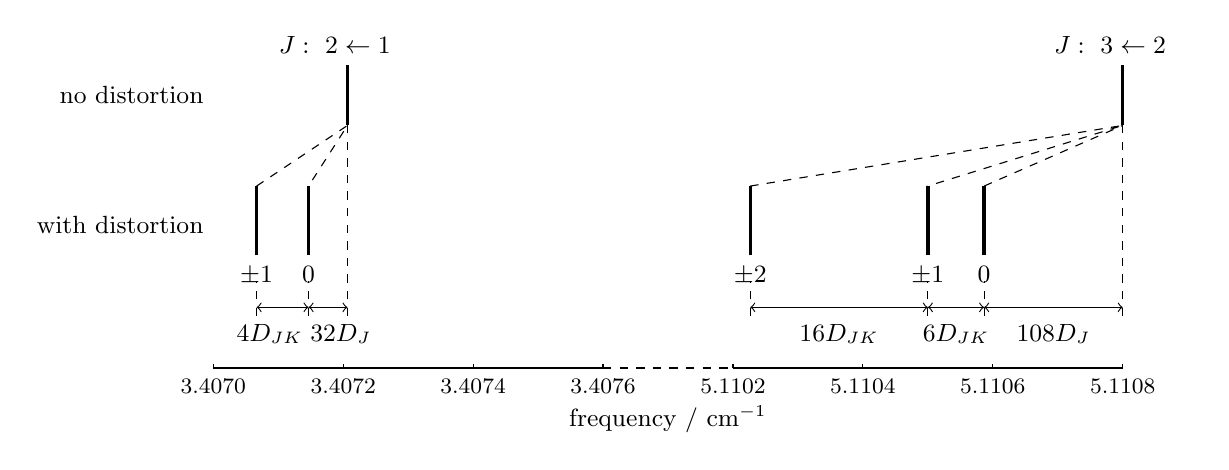
\begin{tikzpicture}[scale=1.1]
            \draw (0,0)--(4.5,0);
            \draw[dashed] (4.5,0)--node[below=1em]{\small frequency /\(\unit{cm}^{-1}\)}(6,0);
            \draw (6,0)--(10.5,0);
            \foreach \i in {0,2,4,6}{
                \draw (0.75*\i,0)--(0.75*\i,0.05)node[below=2pt]{\footnotesize\(3.407\i\)};
            }
            \foreach \i in {2,4,6,8}{
                \draw (4.5+0.75*\i,0)--(4.5+0.75*\i,0.05)node[below=2pt]{\footnotesize\(5.110\i\)};
            }
            \draw[very thick] (1.55,2.8)--(1.55,3.5)node[above]{\small \(J:\ 2\leftarrow 1\quad\)};
            \draw[very thick] (0.5,1.3)node[below]{\small \(\pm 1\)}--(0.5,2.1);
            \draw[very thick] (1.1,1.3)node[below]{\small \(0\)}--(1.1,2.1);
            \draw[very thick] (10.5,2.8)--(10.5,3.5)node[above]{\small \(J:\ 3\leftarrow 2\quad\)};
            \draw[very thick] (6.2,1.3)node[below]{\small \(\pm 2\)}--(6.2,2.1);
            \draw[very thick] (8.25,1.3)node[below]{\small \(\pm 1\)}--(8.25,2.1);
            \draw[very thick] (8.9,1.3)node[below]{\small \(0\)}--(8.9,2.1);
            \draw[dashed] (0.5,2.1)--(1.55,2.8)--(1.1,2.1);
            \draw[dashed] (6.2,2.1)--(10.5,2.8)--(8.25,2.1);
            \draw[dashed] (8.9,2.1)--(10.5,2.8);
            \node at (0,3.15)[left]{\small no distortion};
            \node at (0,1.65)[left]{\small with distortion};
            \draw[dashed] (1.55,0.6)--(1.55,2.8);
            \draw[dashed] (0.5,0.6)--(0.5,1);
            \draw[dashed] (1.1,0.6)--(1.1,1);
            \draw[dashed] (10.5,0.6)--(10.5,2.8);
            \draw[dashed] (6.2,0.6)--(6.2,1);
            \draw[dashed] (8.25,0.6)--(8.25,1);
            \draw[dashed] (8.9,0.6)--(8.9,1);
            \draw[<->] (0.5,0.7)--node[below=2.5pt]{\small \(4D_{JK}\ \ \ \)}(1.1,0.7);
            \draw[<->] (1.1,0.7)--node[below=2.5pt]{\small \(\ \ \ 32D_{J}\)}(1.55,0.7);
            \draw[<->] (6.2,0.7)--node[below=2.5pt]{\small \(16D_{JK}\)}(8.25,0.7);
            \draw[<->] (8.25,0.7)--node[below=2.5pt]{\small \(6D_{JK}\)}(8.9,0.7);
            \draw[<->] (8.9,0.7)--node[below=2.5pt]{\small \(108D_{J}\)}(10.5,0.7);
        \end{tikzpicture}
        \caption{The schematic spectrum showing the effect of centrifugal distortion on the \(J=2\leftarrow 1\) and \(J=3\leftarrow 2\) transitions of \(\mathrm{CH_3F}\). For this molecule, \(\tilde{D}_J=1.96\times 10^{-6}\unit{cm}^{-1}\), \(\tilde{D}_{JK}=1.48\times 10^{-5}\unit{cm}^{-1}\), \(\tilde{A}=5.081\unit{cm}^{-1}\) and \(\tilde{B}=0.5815\unit{cm}^{-1}\). Note the break in the frequency scale --- the change in line positions is very small compared to the separation of the two transitions.}
    \end{figure}
   
    We can also calculate the separation between lines from the same \(J\) value but successive \(K\) values (i.e. \(K\) and \(K+1\)):
    \begin{equation}
        \tilde{\nu}(J,K)-\tilde{\nu}(J,K+1)=2\tilde{D}_{JK}(J+1)(2K+1)\,.
    \end{equation}
    It is clear that this separation increases with both \(K\) and \(J\), as can be seen in the schematic spectrum above.

    \begin{figure}
        \centering
        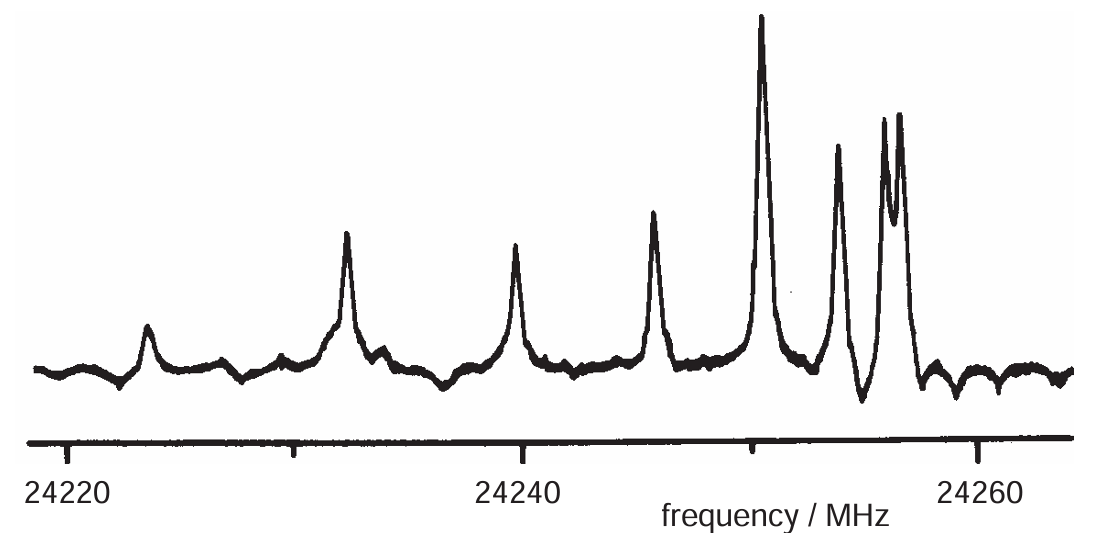
\includegraphics[width=0.7\textwidth]{Centrifugal_distortion.png}
        \caption{The \(J=8\leftarrow 7\) transition of the symmetric top molecule \(\mathrm{SiH_3NCS}\). The scale runs from \(0.8076\) to \(0.8087\unit{cm}^{-1}\). Intensity alternation is due to nuclear spin effects. Figure adapted from Hollas.}
    \end{figure}

    \subsubsection{Linear Molecules}
    The effect of centrifugal distortion on the energy levels of a linear molecule is considerably simpler than for a symmetric top (because it is a one dimensional power series)
    \begin{equation}
        \tilde{E}_J=\tilde{B}J(J+1)-\tilde{D}J^2(J+1)^2\,,
    \end{equation}
    where \(\tilde{D}\) is the positive centrifugal distortion constant.

    Again, the effect of \(\tilde{D}\) is to make levels closer together, and the effect increases with \(J\). The frequency of a transition from \(J''=J\) to \(J'=J+1\) is
    \begin{align}
        \tilde{\nu}_J&=\tilde{E}_{J+1}-\tilde{E}_{J}\notag\\
        &=2\tilde{B}(J+1)-4\tilde{D}(J+1)^3\,.
    \end{align}
    Hence, if we plot \(\tilde{\nu}(J)/(J+1)\) against \((J+1)^2\), we can obtain a straight line with slope \(-4\tilde{D}\) and \(y\)-intercept \(2\tilde{B}\).

    For a diatomic, it is easy to imagine how the ``centrifugal force'' due to rotation stretches the bond thus leading to an increase in the moment of inertia. As commented on above, rather than allowing the rotational constant to be a function of \(J\), we simply add an extra term in \(D\). The value of \(D\) is clearly related to the ease with which the bond can be stretched, which in turn is related to the force constant of the bond and its harmonic frequency, \(\tilde{\omega}\). It can be shown that
    \begin{equation}
        \tilde{D}=\frac{4\tilde{B}^3}{\tilde{\omega}^2}\,.
    \end{equation}
    \subsection{The Stark Effect}
    Molecular and atomic energy levels may be modified when an electric or a magnetic field is applied; as a result the observed spectra will change. These changes may be of help in assigning spectra or may give access to molecular parameters.

    In this section we are going to consider the effect of an electric field on the spectrum of a symmetric top molecule possessing a dipole moment. We shall see that the application of the field results in a splitting of the energy levels, called the \textit{Stark effect}. From the splitting it is possible to determine a value for the dipole moment.
    \subsubsection{Dipole Moment in an Electric Field}
    In classical physics, an electric dipole \(\vb{\mu}\) interacts with electric field \(\vb{E}\) with energy
    \begin{equation}
        -\vb{\mu}\vdot\vb{E}\,.
    \end{equation}
    The value of this dot product depends on the angle \(\theta\) between them and their magnitudes:
    \begin{equation}
        -\mu E_{\text{field}}\cos\theta\,.
    \end{equation}
    We use the subscript to avoid confusion between the electric field and energy.

    \subsubsection{Energy Levels of Symmetric Top in Electric Field}
    Consider a prolate symmetric top, such as \(\mathrm{CH_3F}\), in which the molecular dipole lies along the unique axis \(a\) (the principal \(C_3\) axis).

    \begin{figure}[ht!]
        \centering
        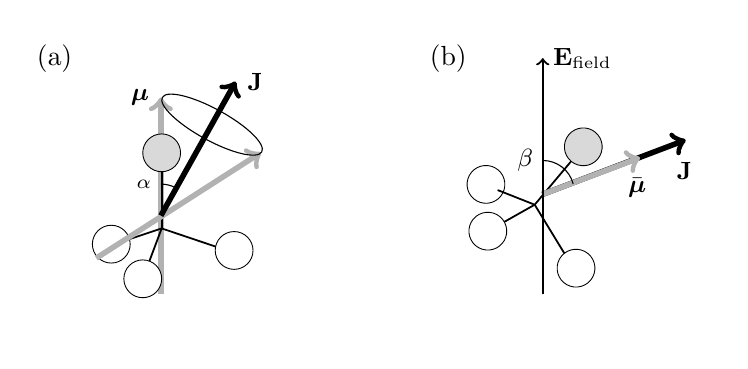
\begin{tikzpicture}
            \node at (0,2) {(a)};
            \draw[->,gray!60,line width=2pt] (1.35,-1)--(1.35,1.5)node[black,left]{\small \(\vb{\mu}\)};
            \node[scale=0.8] at (1.5,0) {\symmtop};
            \draw[->,gray!60,line width=2pt] (0.53,-0.54)--(2.62,0.8);
            \draw[->,line width=2pt] (1.35,0)--(2.3,1.7)node[right]{\small\(\vb{J}\)};
            \node at (2,1.155){\tikz{\draw[rotate=-28.68] (0,0) ellipse (0.72cm and 0.2cm)}};
            \draw (1.35,0.4) arc (90:61.32:0.4);
            \node at (1.35,0.4) [left]{\scriptsize\(\alpha\)};

            \node at (5,2) {(b)};
            \node[rotate=-40] at (6.5,0.4){\tikz{
                \node[scale=0.8] at (1.5,0) {\symmtop};
                \draw[->,line width=2pt] (1.35,0)--(2.3,1.7);
                \draw[->,gray!60,line width=2pt] (1.35,0)--(2,1.155);
            }};
            \draw[thick,->] (6.2,-1)--(6.2,2)node[right]{\small\(\vb{E}_{\text{field}}\)};
            \draw (6.2,0.7) arc (90:15:0.4);
            \node at (6.2,0.7)[left]{\small \(\beta\)};
            \node at (7.4,0.6)[below]{\small \(\bar{\vb{\mu}}\)};
            \node at (8,0.8)[below]{\small \(\vb{J}\)};
        \end{tikzpicture}
    \end{figure}

    Recall that a molecule is rotating about its angular momentum vector \(\vb{J}\), and that in general, this vector is pointing at some angle to the \(a\)-axis. The dipole is thus precessing on a cone at this angle to the direction of \(\vb{J}\), as shown in figure (a) below. As a result of this precession, the dipole is averaged so that only its projection onto \(\vb{J}\) survives; the components perpendicular to \(\vb{J}\) are averaged to zero. Recall the magnitude of the \(\vb{J}\) vector is \(\hbar\sqrt{J(J+1)}\), and its projection on the \(a\)-axis is \(K\), so
    \begin{equation}
        \cos\alpha=\frac{K}{\sqrt{J(J+1)}}\,.
    \end{equation}
    Hence, the averaged dipole moment of the rotating molecule is
    \begin{equation}
        \bar{\vb{\mu}}=\mu\cos\alpha\vu{J}=\frac{\mu K}{\sqrt{J(J+1)}}\vu{\vb{J}}\,.
    \end{equation}

    Now suppose that an electric field is applied and that the molecule is oriented such that \(\vb{J}\) makes an angle \(\beta\) to the electric field direction, as shown in (b). As we have already discussed, the energy of interaction is \(-\bar{\mu}E_{\text{field}}\cos\beta\).

    The vector \(\vb{J}\) cannot point in any direction. Since the applied electric field created a distinct (preferred) direction, the angular momentum must be oriented such that its projection onto the direction of the electric field is \(M_J\) where, as usual, \(M_J\) takes values in integer steps from \(+J\) to \(-J\). Hence, we have
    \begin{equation}
        \cos\beta=\frac{M_J}{\sqrt{J(J+1)}}\,.
    \end{equation}

    Therefore, the energy of interaction is
    \begin{align}
        E_{\text{Stark}}(J,K,M_J)&=-\bar{\mu}E_{\text{field}}\cos\beta\notag\\
        &=-\frac{\mu E_{\text{field}}KM_J}{J(J+1)}\,.\label{Stark_effect}
    \end{align}
    The energy shift caused by the electric field is thus proportional to the field and the dipole moment, and also depends on the three quantum numbers \(J\), \(K\) and \(M_J\).
    
    \subsubsection{Effect on the Spectrum}
    From (\ref{Stark_effect}), we can see immediately that only energy levels with \(K\ne 0\) will be affected by an electric field. Let us consider, as an example, the transition between \(J=1\), \(K=+1\) and \(J=2\), \(K=+1\). In the presence of an electric field the \(J=1\) level will split into three states, with \(M_J=-1,0,1\). The energy shifts will be
    \begin{equation}
        E_{\text{Stark}}(1,1,-1)=\frac{\mu E_{\text{field}}}{2}\quad E_{\text{Stark}}(1,1,0)=0\quad E_{\text{Stark}}(1,1,+1)=-\frac{\mu E_{\text{field}}}{2}\,.
    \end{equation}
    The \(J=2\) level will split into five states with \(M_J\) from \(-2\) to \(+2\); the energy shifts are
    \begin{equation}
        E_{\text{Stark}}(2,1,\pm 2)=\mp\frac{\mu E_{\text{field}}}{3} \quad E_{\text{Stark}}(2,1,\pm 1)=\mp\frac{\mu E_{\text{field}}}{6} \quad E_{\text{Stark}}(2,1,0)=0\,.
    \end{equation}
    
    The splitting of the energy levels is shown in the diagram below (to avoid clutter, the size of the electric field is given the symbol \(E\)).

    Assuming that the electric field is parallel to the electric vector of the radiation (experimentally the most convenient arrangement), the selection rule for \(M_J\) is \(\Delta M_J=0\), so there are three allowed transitions. The single line, observed in the absence of the field, splits symmetrically into three and, from the shifts in the energy levels, it can be seen that the splitting of the lines in the spectrum is \(\mu E_{\text{field}}/3h\) in frequency.
    
    \begin{figure}[ht!]
        \centering
        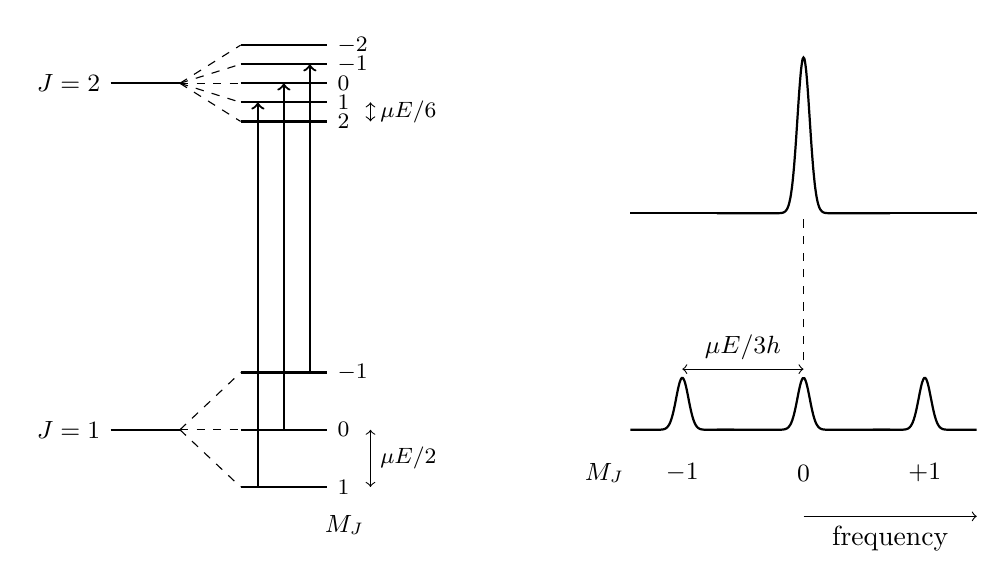
\begin{tikzpicture}[scale=1.1]
            \draw[thick] (0,0)node[left]{\small\(J=1\)}--(0.8,0);
            \draw[thick] (0,4)node[left]{\small\(J=2\)}--(0.8,4);
            \foreach \i in {-1,0,1}{
                \draw[thick] (1.5,-0.66*\i)--(2.5,-0.66*\i)node[right]{\footnotesize\(\i\)};
                \draw[dashed] (0.8,0)--(1.5,-0.66*\i);
                \draw[thick,->] (2-0.3*\i,-0.66*\i)--(2-0.3*\i,4-0.22*\i);
            }
            \foreach \i in {-2,-1,0,1,2}{
                \draw[thick] (1.5,4-0.22*\i)--(2.5,4-0.22*\i)node[right]{\footnotesize\(\i\)};
                \draw[dashed] (0.8,4)--(1.5,4-0.22*\i);
            }
            \node at (2.7,-1.1){\small\(M_J\)};
            \draw[<->] (3,0)--node[right]{\footnotesize\(\mu E/2\)}(3,-0.66);
            \draw[<->] (3,3.56)--node[right]{\footnotesize\(\mu E/6\)}(3,3.78);
            \draw[thick,domain=-1:1, smooth, variable=\x,samples=100] plot ({\x+8}, {2.5+1.8*2.72^(-100*\x*\x)});
            \draw [thick] (6,2.5)--(7,2.5);
            \draw [thick] (9,2.5)--(10,2.5);
            \draw[thick,domain=-1:1, smooth, variable=\x,samples=100] plot ({\x+8}, {0.6*2.72^(-100*\x*\x)});
            \draw[thick,domain=-0.6:0.6, smooth, variable=\x,samples=100] plot ({\x+6.6}, {0.6*2.72^(-100*\x*\x)});
            \draw[thick,domain=-0.6:0.6, smooth, variable=\x,samples=100] plot ({\x+9.4}, {0.6*2.72^(-100*\x*\x)});
            \draw[dashed] (8,0.8)--(8,2.5);
            \draw[<->] (6.6,0.7)--node[above]{\small \(\mu E/3h\)}(8,0.7);
            \node at (5.7,-0.5) {\small \(M_J\)};
            \node at (6.6,-0.5) {\small \(-1\)};
            \node at (8,-0.5) {\small \(0\)};
            \node at (9.4,-0.5) {\small \(+1\)};
            \draw[->] (8,-1)--node[below]{frequency}(10,-1);
        \end{tikzpicture}
    \end{figure}
    
    In general, a transition from a level with quantum numbers \(J\) and \(K\) will split into \((2J+1)\) lines; the splitting (in frequency units) between adjacent lines is
    \begin{equation}
        \frac{2\mu E_{\text{field}}K}{hJ(J+1)(J+2)}\,.
    \end{equation}

    There are two main applications of the Stark effect.
    \begin{enumerate}[topsep=0pt,label=(\roman*)]
        \item Assignment of spectra: assignment means identifying the quantum numbers of the energy levels involved in each transition. By observing the Stark splittings, information on the value of \(J\) can be found.
        \item Measurement of dipole moments: if the magnitude of the electric field is known, then the measured Stark splittings can be used to derive a value for the dipole moment.
    \end{enumerate}
    \subsubsection{Stark Effects for Linear Molecules}
    As mentioned above, linear molecules have no rotation about the internuclear axis, and so effectively \(K=0\) at all times. Hence the energy levels will not be split by the application of an electric field to the first order --- there is thus no first order Stark effect. However, linear molecules do show a \textit{second order Stark effect}, which is where the splitting of the energy levels goes as the square of the electric field strength.\footnote{See, for example, my notes on C7: Further Quantum Mechanics or Principles of Quantum Mechanics.} The effect described for the symmetric top is first order, as it is linear in the field strength.

    \newpage
    \section{Vibrational Spectroscopy}
    Transitions between the set of energy levels associated with molecular vibrations can give rise to absorptions in the infra-red part of the spectrum. Changes in vibrational energy are accompanied by simultaneous changes in rotational energy; as rotational energies are much smaller than vibrational energies, these changes in rotational energy lead to fine structure on the vibrational transitions.

    An analysis of these vibrational transitions and their attendant rotational fine structure gives access to molecular parameters such as vibrational frequencies and rotational constants.
    \subsection{Normal Modes and Symmetry: Revision of Part IB}
    \begin{enumerate}[topsep=0pt,label=(\roman*)]
        \item  A normal mode is a motion in which: (1) the centre of mass remains fixed; (2) the atoms all move in phase at the same frequency; (3) the vibrational potential is harmonic.
        \item A non-linear molecule with \(N\) atoms has \(3N-6\) normal modes, and a linear molecule has \(3N-5\) normal modes.
        \item In the harmonic approximation, each normal mode has a set of energy levels
        \begin{equation}
            \tilde{E}_{v_i}=\left(v_i+\frac{1}{2}\right)\tilde{\omega}_i\,,
        \end{equation}
        where \(v_i=0,1,2,\dots\), and \(\tilde{\omega}_i\) is the vibrational wavenumber of the \(i^{\text{th}}\) normal mode.
        \item Each normal mode transforms as a particular irreducible representation. For a given normal mode \(i\) that transforms as \(\Gamma^{(i)}\)
        \begin{enumerate}[topsep=0pt]
            \item[(a)] The wavefunction of the ground vibrational state (\(v_i=0\)) transforms as the totally symmetric IR, \(\Gamma^{\text{tot. sym.}}\).
            \item[(b)] The first excited state, \(v_i=1\), has the same IR as the normal mode \(\Gamma^{(i)}\).
            \item[(c)] For non-degenerate normal modes the even vibrational states (\(v_i=0,2,4,\dots\)) all transform as \(\Gamma^{\text{tot. sym.}}\), while the odd vibrational states (\(v_i=1,3,5,\dots\)) all transform as \(\Gamma^{(i)}\).
        \end{enumerate}
        \item A transition is allowed in the infra-red if the transition dipole moment between the two states \(v'_i\) and \(v_i\) is non-zero. This will only be so if the following direct product contains the totally symmetric IR:
        \begin{equation}
            \Gamma^{v_i'}\otimes\Gamma^\mu\otimes\Gamma^{v_i}\,,
        \end{equation}
        where \(\Gamma^\mu\) is the IR of the dipole moment operator, \(\hat{\mu}\). \(\Gamma^\mu\) transforms as the Cartesian functions \(x\), \(y\) or \(z\).
        \item A transition will give rise to Raman scattering if, when multiplied out, the following direct product contains the totally symmetric IR:
        \begin{equation}
            \Gamma^{v_i'}\otimes\Gamma^\alpha\otimes\Gamma^{v_i}\,,
        \end{equation}
        where \(\Gamma^\alpha\) is the IR of the polarisability operator, \(\hat{\alpha}\). \(\Gamma^\alpha\) transforms as the Cartesian functions \(x_ix_j\).
    \end{enumerate}
    \subsection{Symmetry of the Vibrational Wavefunction}
    As seen in IB \textit{Introduction to Quantum Mechanics}, for a diatomic the harmonic oscillator wavefunctions depend only on the displacement from equilibrium position \(x=r-r_e\).

    In more complex molecules, a normal mode involves several atoms changing their positions in a concerted way. For a given normal mode \(i\) this motion can be described by a \textit{normal coordinate} \(Q_i\), which is a combination of the displacements of the individual atoms.\footnote{The way to work out the normal coordinates using molecular Hamiltonian is introduced in C7: \textit{Further Quantum Mechanics}. An alternative method using Lagrangian mechanics is in IB Mathematical Methods.}

    For example, for the symmetric stretch of \(\mathrm{CO_2}\) the normal coordinate is
    \begin{equation}
        Q_{\text{sym.str.}}=\frac{1}{\sqrt{2}}(q_{\mathrm{O1}}-q_{\mathrm{O2}})\,.
    \end{equation}
    The \(q\) are mass-weighted coordinates defined as \(q_i=m_i^{1/2}z_i\), where \(z_i\) is the displacement of atom \(i\) from equilibrium position. In this mode, the oxygen atoms move equally and oppositely along the long axis, and the carbon atom does not move.

    The normal coordinate for the antisymmetric stretch is more complex
    \begin{equation}
        Q_{\text{asym.str.}}=\frac{1}{\sqrt{2m_{\mathrm{C}}+4m_{\mathrm{O}}}}\left(m_{\mathrm{C}}^{1/2}q_{\mathrm{O1}}-2m_{\mathrm{O}}^{1/2}q_{\mathrm{C}}+m_{\mathrm{C}}^{1/2}q_{\mathrm{O2}}\right)\,.
    \end{equation}
    In this normal coordinate the two oxygen atoms move in the same direction and the carbon moves in the opposite direction. The amount each atom moves depends on its mass. For the bending mode, displacements along \(x\) and \(y\) would also appear in the normal coordinate.

    For a given normal mode the potential energy function, and hence the associated wavefunctions, depends on just this one variable, \(Q_i\). It therefore follows that the harmonic oscillator wavefunctions are also the wavefunctions for any normal mode provided we replace \(q\) with the normal coordinate for mode \(i\), \(Q_i\).
    
    In Part IB \textit{Symmetry and Bonding} we used direct products to work out the symmetry of the vibrational wavefunctions for non-degenerate normal modes. Here, we will briefly recap the argument and then go on to extend it to the more complex case of degenerate normal modes.
    
    \subsubsection{Non-degenerate Normal Modes}
    Suppose the ground state wavefunction of the non-degenerate \(i^{\text{th}}\) normal mode, with \(v_i=0\), is \(\psi_0=\exp(-\frac{1}{2}Q_i^2)\). Suppose also normal mode, and hence the normal coordinate \(Q_i\), transforms as the one-dimensional irreducible representation \(\Gamma^{(i)}\), then \(Q_i^2\) transforms as
    \begin{equation}
        \Gamma^{(i)}\otimes \Gamma^{(i)}=\Gamma^{\text{tot.sym.}}\,.
    \end{equation}
    Since \(Q_i^2\) is invariant under any symmetry operation, \(\exp(-\frac{1}{2}Q_i^2)\) is invariant as well, so the ground state wavefunction \(\psi_0\) transforms as the totally symmetric irreducible representation for any non-degenerate mode.

    The first excited state wavefunction is
    \begin{equation}
        \psi_1=2Q_i\exp\left(-\frac{1}{2}Q_i^2\right)\,,
    \end{equation}
    so it transforms as
    \begin{equation}
        \Gamma^{(i)}\otimes \Gamma^{\text{tot.sym.}}=\Gamma^{(i)}\,.
    \end{equation}

    The next wavefunction is
    \begin{equation}
        \psi_2=(4Q_i^2-2)\exp\left(-\frac{1}{2}Q_i^2\right)\,.
    \end{equation}
    We have \(Q_i^2\) and the exponential term both transforming as totally symmetric irreducible representation, and all the scalars are also totally symmetric. Hence, the doubly excited wavefunction transforms as \(\Gamma^{\text{tot.sym.}}\).

    Generally, the \(k^{\text{th}}\) vibrational wavefunction is
    \begin{equation}
        \psi_k(Q_i)=H_k(Q_i)\exp\left(-\frac{1}{2}Q_i^2\right)\,,
    \end{equation}
    where \(H_k\) is the \(k^{\text{th}}\) Hermite polynomial. It is easy to see that the odd orders of \(Q_i\) transforms as \(\Gamma^{(i)}\), while the even orders of \(Q_i\) transforms as \(\Gamma^{\text{tot.sym.}}\). Since the odd-order Hermite polynomial only contain odd powers, while the even order Hermite polynomials only contain even powers, we arrive at this simple conclusion:

    \fbox{\begin{minipage}{0.9\textwidth}
        For non-degenerate normal modes the wavefunctions with even \(v\) transform as the totally symmetric irreducible representation, and those with odd \(v\) have the same symmetry as the normal mode.
    \end{minipage}}

    \subsubsection{Degenerate Normal Modes}
    The symmetries of the wavefunctions of degenerate normal modes are rather more complex to deal with, and are discussed in appendix \cref{Chap:symmetry_degenerate_mode}. Here we state the results.

    Suppose that a particular degenerate normal mode transforms as \(\Gamma^{(i)}\).
    \begin{enumerate}[topsep=0pt,label=(\roman*)]
        \item the ground state wavefunction transforms as the totally symmetric irreducible representation \(\Gamma^{\text{tot.sym.}}\).
        \item the wavefunction of the first excited state, in which there is one quantum of excitation in one of the degenerate normal modes, transforms as \(\Gamma^{(i)}\).
    \end{enumerate}

    Now consider the doubly excited states. Consider the doubly degenerate \(E\) mode of \(\mathrm{NH_3}\), point group \(C_{3v}\). The direct product of \(E\) is
    \begin{equation}
        E\otimes E=(2,-1,0)\otimes(2,-1,0)=(4,1,0)=E\oplus A_2\oplus A_1\,.
    \end{equation}
    Note the direct product of two two-dimensional irreducible representations necessarily gives a four-dimensional result.

    We can get this result by reading the direct product tables. A selection of those is shown in \cref{Chap:direct_product}. We can see that, in the table, \(E\otimes E=E\oplus [A_2]\oplus A_1\). The IR in the bracket arises from the \textit{antisymmetrised square}, and the others are from the \textit{symmetrised square}. The details are non-examinable, but it turns out that the symmetries of the vibrational wavefunctions are given only by those IRs arising from the symmetrised square.\footnote{The detail is too much to fit in the margin, or even in the appendix, so it is in a separate course. See B8: \textit{Symmetry}.} For the present case, these IRs are \(A_1\oplus E\).

    Therefore, we have the rules
    \begin{enumerate}[topsep=0pt]
        \item[(iii)] the irreducible representation spanned by the wavefunction of the doubly excited state is found by computing the direct product \(\Gamma^{(i)}\otimes\Gamma^{(i)}\), and then selecting the ones corresponding to the \textit{symmetrised square}.
        \item[(iv)] the IRs of further excited states are computed by taking more direct products and selecting the symmetrised ones.
    \end{enumerate}

    As we have seen, the second excited state of the doubly-degenerate \(E\) mode in \(\mathrm{NH_3}\) transforms as \(A_1\oplus E\). The total dimensionality is 3 since this state has two quanta of excitation, which can be arranged amongst the two degenerate normal modes in three different ways:
    \begin{equation}
        (1,1)\,,\ (2,0)\,,\text{ or } (0,2)\,.
    \end{equation}
    Because these vibrations form a degenerate pair, these arrangements all have the same energy. There are only three possible arrangements of the quanta because there is only one way of assigning one quantum of excitation to each normal mode.

    Note that the direct product of an IR with itself always contains the totally symmetric IR, and that this is part of the symmetrised square.
    \subsubsection{Overall Symmetry of the Vibrational Wavefunction}
    So far we have described how to find the symmetry of the vibrational wavefunctions associated with a particular normal mode. However, multiple vibrational modes may be excited at the same time in a molecule. The overall symmetry of the vibrational wavefunction of the molecule is easily calculated by taking direct products.

    Suppose that for the first normal mode the molecule is in the vibrational energy level with quantum number \(v_1\), and that the irreducible representation of the corresponding wavefunction is \(\Gamma^{v_1}\); likewise for the second normal mode the quantum number is \(v_2\) and the IR is \(\Gamma^{v_2}\), and so on for all the modes. We commonly denote such states by
    \begin{equation}
        (v_1,v_2,v_3,\dots,v_n)\,,
    \end{equation}
    provided that we give an order of the vibrational modes. The irreducible representation of the overall vibrational wavefunction is given by the direct product
    \begin{equation}
        \Gamma_{\text{overall}}=\Gamma^{v_1}\otimes\Gamma^{v_2}\otimes\dots\otimes\Gamma^{v_n}
    \end{equation}
    This works because, by hypothesis, the normal modes are independent of one another.

    Since the ground state wavefunction of any normal mode transforms as the totally symmetric irreducible representation, it follows that for a molecule in which none of the vibrational modes are excited --- the overall ground state in which all the \(v_i\) are zero the overall vibrational wavefunction also transforms as the totally symmetric irreducible representation. Also, if just one normal mode is excited to the \(v=1\) state, and all of the other normal modes have \(v=0\), it follows that the overall vibrational wavefunction has the same irreducible representation as the normal mode which is excited.
    
    \subsection{Determining Allowed Transitions using Symmetry}
    Again, assuming the molecule is a harmonic oscillator, the harmonic selection rules apply, which are
    \begin{enumerate}[topsep=0pt,label=(\roman*)]
        \item The dipole moment must change as the normal coordinate changes about the equilibrium.
        \item \(\Delta v_i=\pm 1\).
    \end{enumerate}
    Note the second condition means the quantum number of only one mode is allowed to change by one. In the presence of anharmonicity, transitions with higher values of \(\Delta v\) are weakly allowed, as are transitions in which more than one mode changes quantum number.

    The intensity of an infra-red transition between vibrational states \(i\) and \(j\) depends on the \textit{transition moment}
    \begin{equation}
        R_{ij}=\int\dd{\tau}\psi_i^*\hat{\mu}\psi_j\,.
    \end{equation}
    This will be non-zero only if the integrand, or some part of it, transforms as the totally symmetric irreducible representation. All we need to do is compute the direct product
    \begin{equation}
        \Gamma_i\otimes\Gamma^\mu\otimes\Gamma_j
    \end{equation}
    to see if it contains \(\Gamma^{\text{tot.sym}}\).

    \subsubsection{Fundamental Transition}
    A fundamental transition is a process in which the molecule goes from the vibrational ground states of all the normal modes to the first excited state of just one normal mode.
    \begin{equation}
        (0,0,\dots,0,\dots,0)\to(0,0,\dots,\underbrace{1}_{v_i},\dots,0)\,.
    \end{equation}

    Since we know that the ground state transforms as \(\Gamma^{\text{tot.sym}}\) and the first excited state of mode \(i\) transforms as \(\Gamma^{(i)}\), the direct product we need to evaluate is
    \begin{equation}
        \Gamma^{(i)}\otimes\Gamma^\mu\otimes\Gamma^{\text{tot.sym.}}\,.
    \end{equation}
    This will contain the totally symmetric irreducible representation if and only if \(\Gamma^{(i)}\) is the same as (some part of) \(\Gamma^\mu\). Hence the rule:

    \fbox{\begin{minipage}{0.9\textwidth}
        A fundamental transition is allowed when the symmetry of the activated normal mode matches that of \(x\), \(y\) or \(z\).

        If the fundamental is allowed, the normal mode is said to be \textit{infra-red active}.
    \end{minipage}}

    As an example, \(\mathrm{H_2O}\ (C_{2v})\) has three normal modes: two of symmetry \(A_1\) and one of symmetry \(B_2\). The fundamentals of \(A_1\) modes are allowed as \(z\) transforms like \(A_1\), and the fundamental of \(B_2\) is also allowed as \(y\) transforms like \(B_2\).

    For the \(B_2\) mode, the triple direct product which gives rise to the totally symmetric irreducible representation is
    \begin{equation}
        \underbrace{B_2}_{\Gamma^{(i)}}\otimes\underbrace{B_2}_{\Gamma^y}\otimes\underbrace{A_1}_{\Gamma^{\text{tot.sym.}}}\,.
    \end{equation}
    The \(y\) component of the dipole is involved, and so the \textit{transition dipole} is said to be along \(y\). We can see that in the \(B_2\) mode, the dipole indeed changes along the \(y\) direction. We say such a transition is \textit{perpendicular} since the transition dipole is perpendicular to the principal axis (\(z\) axis).

    For the \(A_1\) modes, the \(z\) component of the dipole is involved, so the transition dipole is along \(z\) and we describe it as \textit{parallel}.

    \begin{figure}
        \centering
        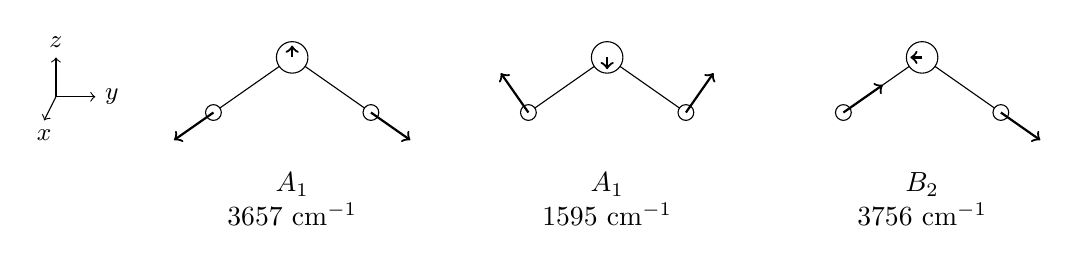
\begin{tikzpicture}
            \draw[->] (0,0)--(0.5,0)node[right]{\small\(y\)};
            \draw[->] (0,0)--(0,0.5)node[above]{\small \(z\)};
            \draw[->] (0,0)--(-0.15,-0.3)node[below]{\small \(x\)};
            \draw (2,-0.2)--(3,0.5)--(4,-0.2);
            \draw[fill=white] (3,0.5) circle (0.2);
            \draw[fill=white] (2,-0.2) circle (0.1);
            \draw[fill=white] (4,-0.2) circle (0.1);
            \draw[thick,->] (2,-0.2)--(1.5,-0.55);
            \draw[thick,->] (4,-0.2)--(4.5,-0.55);
            \draw[thick,->] (3,0.5)--(3,0.65);
            \node[align=center] at (3,-1.3){\(A_1\) \\ \(3657\unit{cm}^{-1}\)};

            \draw (6,-0.2)--(7,0.5)--(8,-0.2);
            \draw[fill=white] (7,0.5) circle (0.2);
            \draw[fill=white] (6,-0.2) circle (0.1);
            \draw[fill=white] (8,-0.2) circle (0.1);
            \draw[thick,->] (6,-0.2)--(5.65,0.3);
            \draw[thick,->] (8,-0.2)--(8.35,0.3);
            \draw[thick,->] (7,0.5)--(7,0.35);
            \node[align=center] at (7,-1.3){\(A_1\) \\ \(1595\unit{cm}^{-1}\)};

            \draw (10,-0.2)--(11,0.5)--(12,-0.2);
            \draw[fill=white] (11,0.5) circle (0.2);
            \draw[fill=white] (10,-0.2) circle (0.1);
            \draw[fill=white] (12,-0.2) circle (0.1);
            \draw[thick,->] (10,-0.2)--(10.5,0.15);
            \draw[thick,->] (12,-0.2)--(12.5,-0.55);
            \draw[thick,->] (11,0.5)--(10.85,0.5);
            \node[align=center] at (11,-1.3){\(B_2\) \\ \(3756\unit{cm}^{-1}\)};
        \end{tikzpicture}
        \caption{Normal modes of water, \(C_{2v}\).}
    \end{figure}
    
    A useful distinction is made between transitions allowed by harmonic selection rule and other transitions that are shown to be allowed by symmetry arguments --- these are said to be \textit{symmetry allowed}. Transitions allowed by selection rules are necessarily symmetry allowed, but there will be transitions not allowed by harmonic selection rules but are nevertheless symmetry allowed.

    \subsubsection{Overtones}
    Transitions from the overall ground state to a state with \(v_i=2,3,\dots\) for a particular normal mode is called an \textit{overtone}. For example, a \textit{first overtone} is
    \begin{equation}
        (0,0,\dots,0,\dots,0)\to(0,0,\dots,\underbrace{2}_{v_i},\dots,0)\,,
    \end{equation}
    and a second overtone is \((0,0,\dots,0,\dots,0)\to(0,0,\dots,3,\dots,0)\) and so on. These transitions are forbidden by harmonic selection rule but are nevertheless frequently observed as a result of anharmonicity.

    Whether or not a particular overtone is allowed is again determined by evaluating the triple direct product
    \begin{equation}
        \Gamma^{v_i}\otimes\Gamma^\mu\otimes\Gamma^{\text{tot.sym}}\,.
    \end{equation}

    For non-degenerate modes, simple conclusions can be made. The second excited state transforms as the totally symmetric irreducible representation, so a first overtone will be allowed only if one of the Cartesian functions (\(x\), \(y\) or \(z\)) transforms as the totally symmetric irreducible representation. The third excited state transforms as the same irreducible representation as the first excited state, so it will be allowed if the fundamental is allowed.

    \subsubsection{Hot Bands}
    \textit{Hot bands} are transitions from states other than the ground state. They are so-called because their intensity increases as the sample is heated, accounting for the increasing population of the excited vibrational states. We again use the triple direct product to determine whether they are allowed or not.
    
    \subsubsection{Combination Lines}
    A \textit{combination line} is a transition in which the quantum number of more than one normal mode changes. This is allowed due to anharmonicity.

    \begin{figure}[ht!]
        \centering
        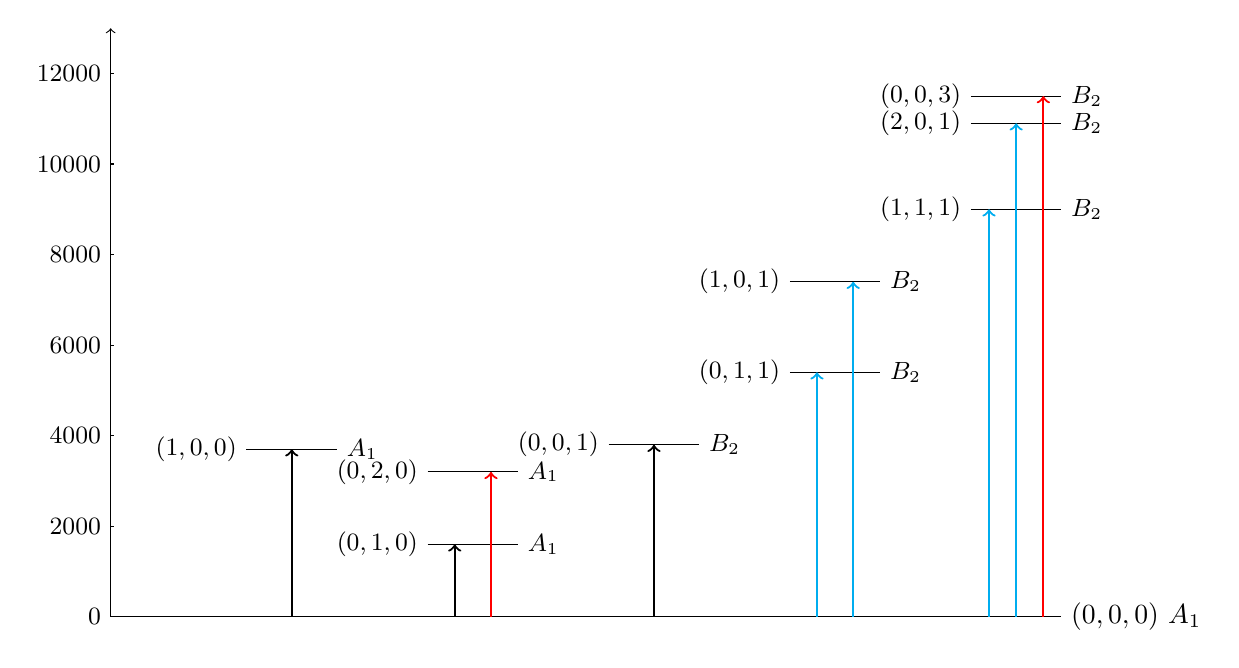
\begin{tikzpicture}[scale=1.15]
            \draw[->] (0,0)--(0,6.5);
            \foreach \i in {0,2000,4000,6000,8000,10000,12000}{
                \draw (0,\i/2000)node[left]{\small \(\i\)}--(0.04,\i/2000);
            }
            \draw (1.5,1.85)node[left]{\small\((1,0,0)\)}--(2.5,1.85)node[right]{\small\(A_1\)};
            \draw (3.5,1.6)node[left]{\small\((0,2,0)\)}--(4.5,1.6)node[right]{\small\(A_1\)};
            \draw (3.5,0.8)node[left]{\small\((0,1,0)\)}--(4.5,0.8)node[right]{\small\(A_1\)};
            \draw (5.5,1.9)node[left]{\small\((0,0,1)\)}--(6.5,1.9)node[right]{\small\(B_2\)};
            \draw (7.5,2.7)node[left]{\small\((0,1,1)\)}--(8.5,2.7)node[right]{\small\(B_2\)};
            \draw (7.5,3.7)node[left]{\small\((1,0,1)\)}--(8.5,3.7)node[right]{\small\(B_2\)};
            \draw (9.5,4.5)node[left]{\small\((1,1,1)\)}--(10.5,4.5)node[right]{\small\(B_2\)};
            \draw (9.5,5.45)node[left]{\small\((2,0,1)\)}--(10.5,5.45)node[right]{\small\(B_2\)};
            \draw (9.5,5.75)node[left]{\small\((0,0,3)\)}--(10.5,5.75)node[right]{\small\(B_2\)};
            \draw (0,0)--(10.5,0)node[right]{\((0,0,0)\ A_1\)};
            \draw[->,thick] (2,0)--(2,1.85);
            \draw[->,thick] (3.8,0)--(3.8,0.8);
            \draw[->,thick,red] (4.2,0)--(4.2,1.6);
            \draw[->,thick] (6,0)--(6,1.9);
            \draw[->,thick,cyan] (7.8,0)--(7.8,2.7);
            \draw[->,thick,cyan] (8.2,0)--(8.2,3.7);
            \draw[->,thick,cyan] (9.7,0)--(9.7,4.5);
            \draw[->,thick,cyan] (10,0)--(10,5.45);
            \draw[->,thick,red] (10.3,0)--(10.3,5.75);
        \end{tikzpicture}
        \caption{Some fundamentals (black), overtones (red), and combination lines (cyan) for \(\mathrm{H_2O}\). All of them are symmetry allowed.}
    \end{figure}
    \subsubsection*{A Note of Caution}
    The symmetry argument is simple and powerful, but it needs some care to be applied. It only predicts whether a transition is possible or not, but it does not predict how strong it will be.

    For a transition to be strong, the lower level needs to be significantly occupied. In practice, this means that for small molecules, only the transitions from the vibrational ground states are easily observable. Moreover, it is possible for the transition moment integral to vanish even if the transition is symmetry allowed (and here comes the harmonic selection rule \(\Delta v=\pm 1\)).

    The vibrations of real molecules are not strictly harmonic and so the \(\Delta v=\pm 1\) rule does not apply rigidly. Under these circumstances a transition which is allowed in principle by symmetry considerations, and also comes from a significantly populated lower level, may be visible. For example, the first overtone is commonly seen although typically with about one tenth of the intensity of the fundamental (on account of the lower transition moment).
    
    \subsubsection{Fermi Resonance}
    In some spectra an overtone or combination line may appear with an unexpectedly high intensity as a result of \textit{Fermi resonance}.

    This is best explained with an example. The linear isocyanate anion \(\mathrm{[NCO]^-}\ (C_{\infty v})\) has four normal modes with symmetries \(\Sigma^+\), \(\Pi\) and \(\Sigma^+\). The first \(\Sigma^+\) mode is classified as \(\mathrm{C-O}\) stretch and has a frequency of \(1240\unit{cm}^{-1}\). The \(\Pi\) mode is a bending mode with frequency \(630\unit{cm}^{-1}\).

    Therefore, the \((1,0,0)\) state has symmetry \(\Sigma^+\) and the \((0,2,0)\) state has symmetry \(\Pi\otimes\Pi=\Sigma^+\oplus\Delta\). In the absence of any special effects, we expect the \((1,0,0)\) state to be \(1240\unit{cm}^{-1}\) above the \((0,0,0)\) ground state, and the \((0,2,0)\) state to be \(2\times 630=1260\unit{cm}^{-1}\) above the ground state. We therefore have two levels with similar energies and the same symmetry \(\Sigma^+\). We therefore expect the two states to interact and mix. The result is they ``push one another apart'', as shown in the diagram below.
    \begin{figure}[ht!]
        \centering
        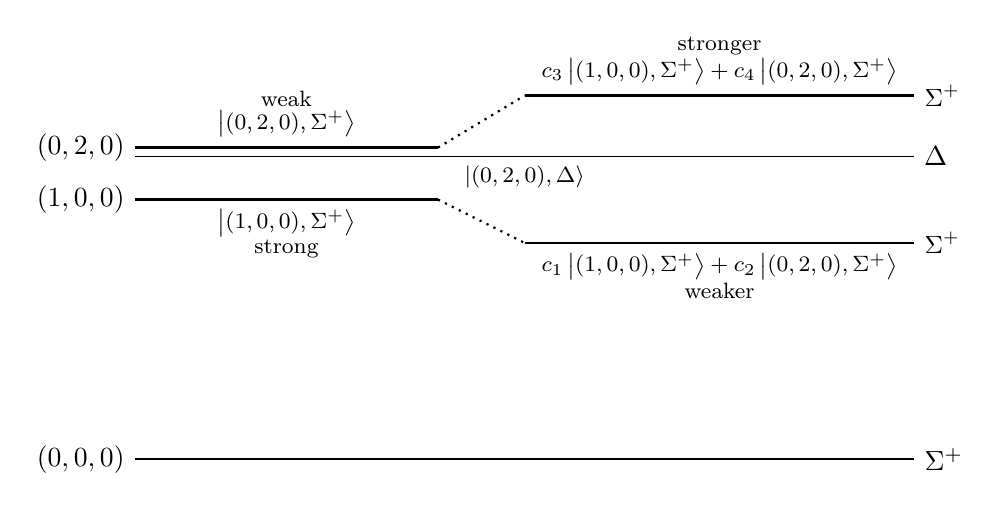
\begin{tikzpicture}[scale=1.1]
            \draw[thick](0,0)node[left]{\((0,0,0)\)}--(9,0)node[right]{\(\Sigma^+\)};
            \draw[thick] (0,3)node[left]{\((1,0,0)\)}--node[below]{\footnotesize \(\ket{(1,0,0),\Sigma^+}\)}node[below=11pt]{\footnotesize strong}(3.5,3);
            \draw (0,3.5)--node[below]{\footnotesize \(\ket{(0,2,0),\Delta}\)}(9,3.5)node[right]{\(\Delta\)};
            \draw[thick] (0,3.6)node[left]{\((0,2,0)\)}--node[above]{\footnotesize \(\ket{(0,2,0),\Sigma^+}\)}node[above=11pt]{\footnotesize weak}(3.5,3.6);
            \draw[dotted,thick] (3.5,3)--(4.5,2.5);
            \draw[thick] (4.5,2.5)--node[below]{\footnotesize \(c_1\ket{(1,0,0),\Sigma^+}+c_2\ket{(0,2,0),\Sigma^+}\)}node[below=11pt]{\footnotesize weaker}(9,2.5)node[right]{\small \(\Sigma^+\)};
            \draw[dotted,thick] (3.5,3.6)--(4.5,4.2);
            \draw[thick] (4.5,4.2)--node[above]{\footnotesize \(c_3\ket{(1,0,0),\Sigma^+}+c_4\ket{(0,2,0),\Sigma^+}\)}node[above=11pt]{\footnotesize stronger}(9,4.2)node[right]{\small \(\Sigma^+\)};
        \end{tikzpicture}
    \end{figure}

    The transition from \((0,0,0)\) to \((1,0,0)\) is an allowed fundamental transition and is expected to be strong. The transition from \((0,0,0)\) to \((0,2,0)\ \Sigma^+\) is symmetry allowed but as this transition is an overtone it is expected to be much weaker. The transition intensity is proportional to the square of the transition moment, so we have
    \begin{equation}
        \mel{(1,0,0),\Sigma^+}{\hat{\mu}}{(0,0,0),\Sigma^+}>\mel{(0,2,0),\Sigma^+}{\hat{\mu}}{(0,0,0),\Sigma^+}
    \end{equation}
    Therefore, when the mixing of states happens, the intensities of transitions are also averaged out, and as a result, the transition to the (mainly) \((0,2,0)\) state becomes stronger.
    \begin{equation}
        \underbrace{\left(c_3\bra{(1,0,0),\Sigma^+}+c_4\bra{(0,2,0),\Sigma^+}\right)\hat{\mu}\ket{(0,0,0),\Sigma^+}}_{R_{ij}\text{ after mixing}}>\underbrace{\mel{(0,2,0),\Sigma^+}{\hat{\mu}}{(0,0,0),\Sigma^+}}_{R_{ij}\text{ without mixing}}\,.
    \end{equation}
    Experimentally, we then see two strong lines at \(1201\unit{cm}^{-1}\) and \(1282\unit{cm}^{-1}\).

    This intensity borrowing with level repulsion is known as Fermi resonance.

    \subsection{Rotational Fine Structure}
    As for diatomics, the vibrational transitions for more complex molecules are accompanied by simultaneous changes in rotational energy which lead to fine structure in the spectrum. Analysis of the fine structure will give structural information in the form of rotational constants. In addition, the form of the fine structure tells us something about the symmetry of the vibrational levels (and hence the symmetry of the normal mode) involved; this information can be useful in assigning the vibrational spectrum.
    \subsubsection{Linear Molecules}
    The allowed vibrational transitions in such molecules come in two broad types:
    \begin{enumerate}[topsep=0pt,label=(\roman*)]
        \item \(\Sigma-\Sigma\) transitions, which are classified as parallel transitions. The transition dipole is along \(z\). \(P\) and \(R\) branches are seen.
        \item \(\Sigma-\Pi\) transitions, which are classified as perpendicular transitions. The transition dipole is along \((x,y)\). \(P\), \(Q\), and \(R\) branches are seen.
    \end{enumerate}
    \subsubsection*{Rotational Fine Structure for \texorpdfstring{\(\bm{\Sigma-\Sigma}\)}{Σ-Σ} Transitions}
    For these transitions the selection rules for the rotational energy levels are
    \begin{equation}
        \Delta J=-1\,:\ P\text{ branch}\,,\qquad\Delta J=+1\,:\ R\text{ branch.}
    \end{equation}
    These are identical to those for heteronuclear diatomics and so the resulting \(P,R\) branch structure is the same. It can be analysed using the method of combination differences to give values for the rotational constants \(B_0\) and \(B_1\).
    
    \begin{figure}
        \centering
        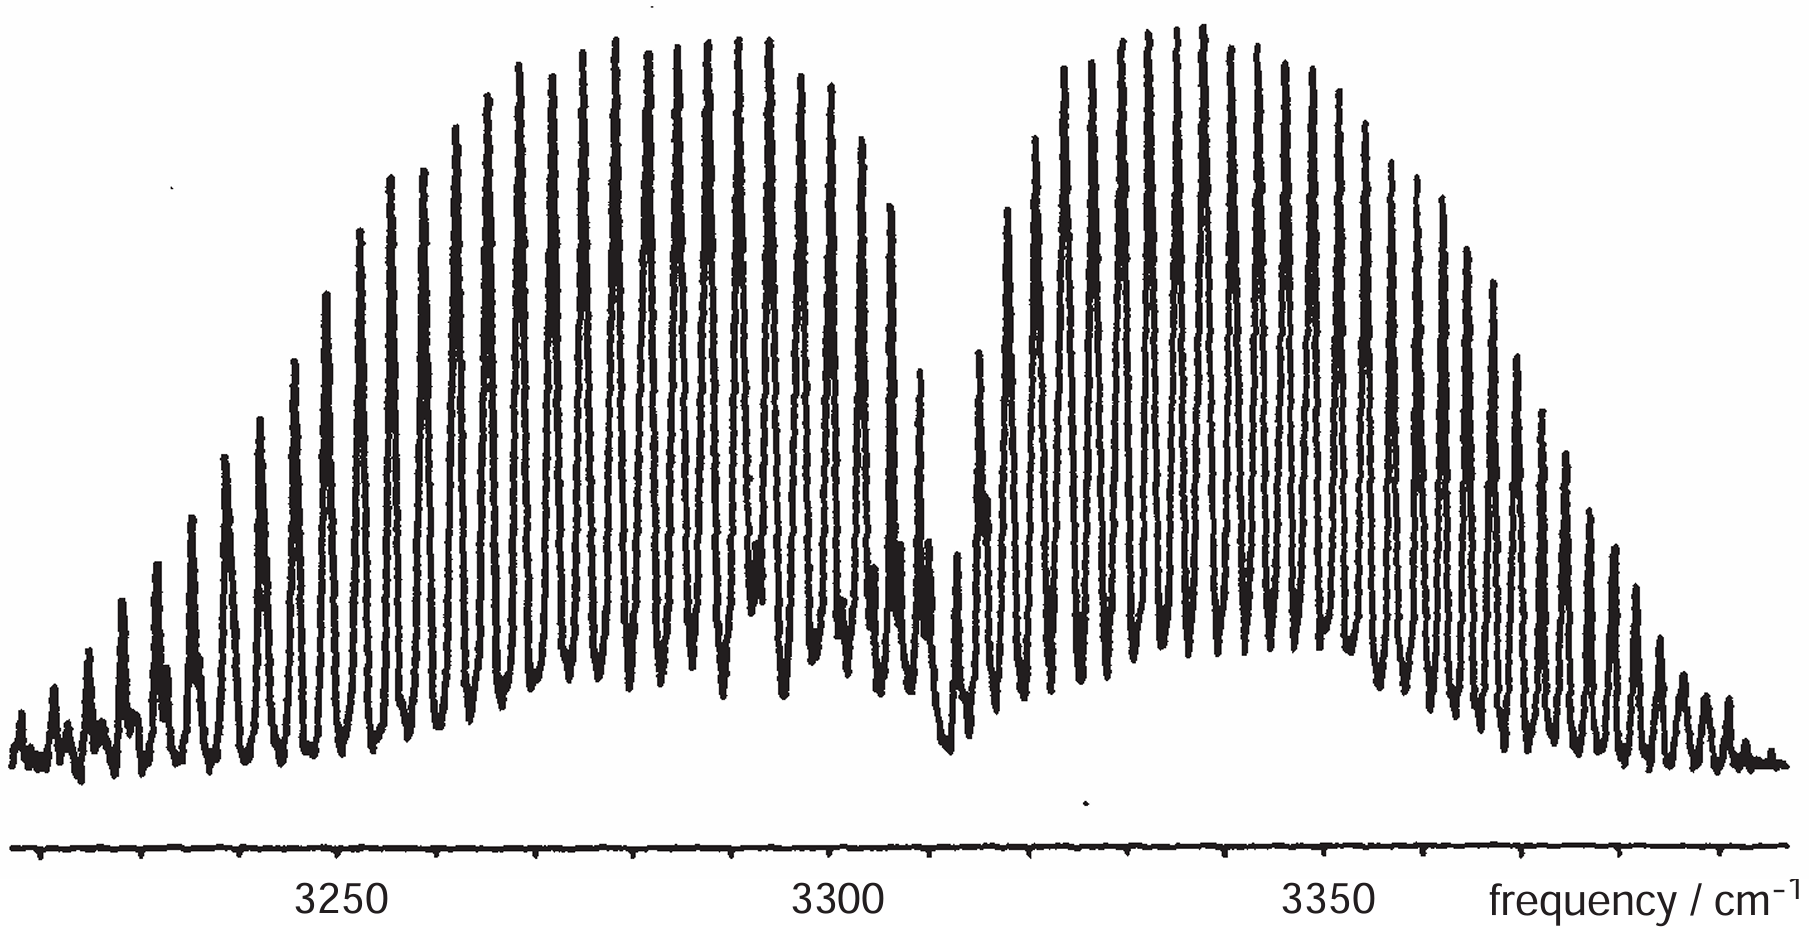
\includegraphics[width=0.7\textwidth]{HCN_vibrot_sigma.png}
        \caption{An experimental spectrum of the rotational structure associated with the fundamental of a \(\Sigma^+\) mode of \(\mathrm{HCN}\), adapted from Banwell; the \(P\) and \(R\) branches are clearly visible.}
    \end{figure}
    \subsubsection*{Rotational Fine Structure for \texorpdfstring{\(\bm{\Sigma-\Pi}\)}{Σ-Π} Transitions}
    For these transitions the selection rules for the rotational energy levels are
    \begin{equation}
        \Delta J=-1\,:\ P\text{ branch}\,,\qquad\Delta J=0\,:\ Q\text{ branch}\,,\qquad\Delta J=+1\,:\ R\text{ branch.}
    \end{equation}
    The frequencies of the lines in the \(Q\) branch can easily be shown to be
    \begin{equation}
        \tilde{\nu}_Q(J)=\tilde{\omega_0}+J(J+1)(\tilde{B}_1-\tilde{B}_0)\,.
    \end{equation}
    Recall that \(\tilde{B}_1\) and \(\tilde{B}_0\) are not very different, so the different lines in the \(Q\) branch are not as widely separated as those in the \(P\) and \(R\) branches. Indeed, when recorded at moderate resolution it is not uncommon for the \(Q\) branch lines not to be resolved from one another but simply to ``pile up'' and give a strong feature in the centre of the band.
    \begin{figure}
        \centering
        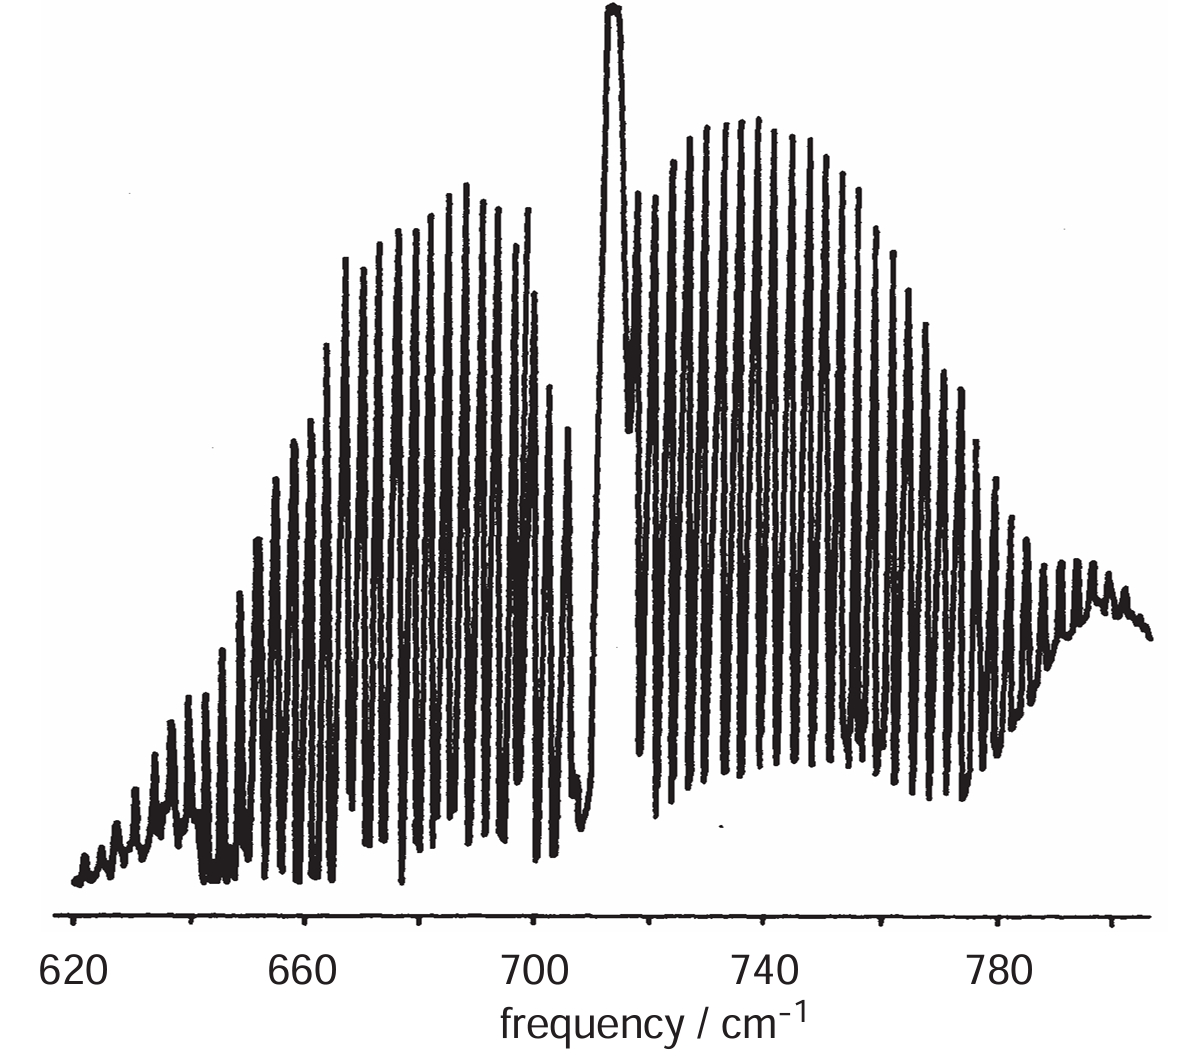
\includegraphics[width=0.5\textwidth]{HCN_vibrot_pi.png}
        \caption{An experimental spectrum of the rotational structure associated with the fundamental \(\Pi\) bending mode of \(\mathrm{HCN}\), adapted from Banwell; the intense \(Q\) branch, made up of many overlapping lines, is clearly visible in the centre of the band.}
    \end{figure}

    \subsubsection{Symmetric Tops}
    As with linear molecules, the nature of the rotational fine structure depends on the symmetry of the vibrational wavefunctions involved. Broadly, we again need to classify the vibrational transition as perpendicular or parallel.

    Throughout this section, we will use \(\mathrm{CH_3I}\) as an example. It is a prolate symmetric top with 3 \(A_1\) and 3 \(E\) normal modes, all of which are IR active. In \(C_{3v}\), \(z\) transforms as \(A_1\), so the \(A_1\) modes are parallel, and \((x,y)\) transforms as \(E\), so the \(E\) modes are perpendicular.

    \subsubsection*{Parallel Transitions}
    For parallel transitions the selections rules for the rotational quantum numbers are
    \begin{equation}
        \Delta J=0,\pm 1\quad \Delta K=0
    \end{equation}
    with the exception that for \(K=0\), \(\Delta J=0\) is not allowed. For each value of \(K\) we thus expect there to be a \(P\), \(Q\), and \(R\) branch (with the exception of \(K=0\) for which there is no \(Q\) branch).

    Recall that the rotational energies for a prolate symmetric top are given by (ignoring centrifugal distortion)
    \begin{equation}
        \tilde{E}_{J,K}=\tilde{B}J(J+1)+(\tilde{A}-\tilde{B})K^2\,.
    \end{equation}
    It is clear that, as \(\Delta K=0\), the term in \((\tilde{A}-\tilde{B}\)) does not affect the positions of the lines and so the \(P\), \(Q\), and \(R\) branches have exactly the same frequency for any value of \(K\). So, what we will see is a simple \(PQR\)-band structure, similar to that for a \(\Sigma-\Pi\) transition of a linear molecule.

    \begin{figure}
        \centering
        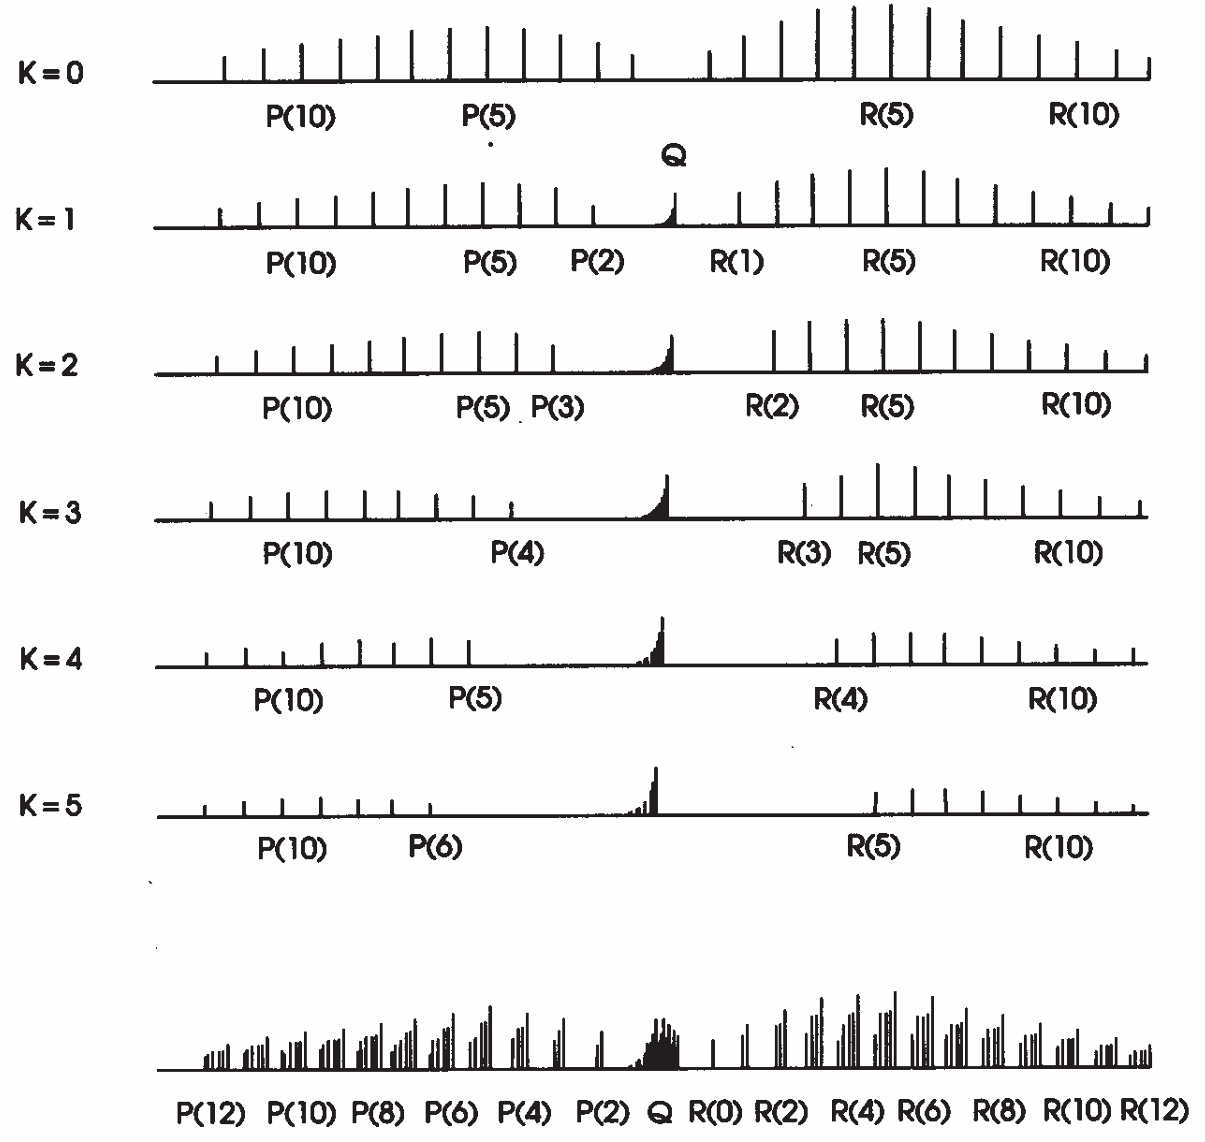
\includegraphics[width=0.7\textwidth]{prolate_top_parallel.png}
        \caption{A schematic spectrum for a parallel transition of a prolate top, adapted from Bernath. The \(P\), \(Q\), and \(R\) branches with different \(K\) values partly overlap. Note that since \(K\) cannot be larger than \(J\), those lines from levels with \(J<K\) are missing from the branches, and that there is no \(Q\) branch for \(K=0\).}
    \end{figure}

    \begin{figure}
        \centering
        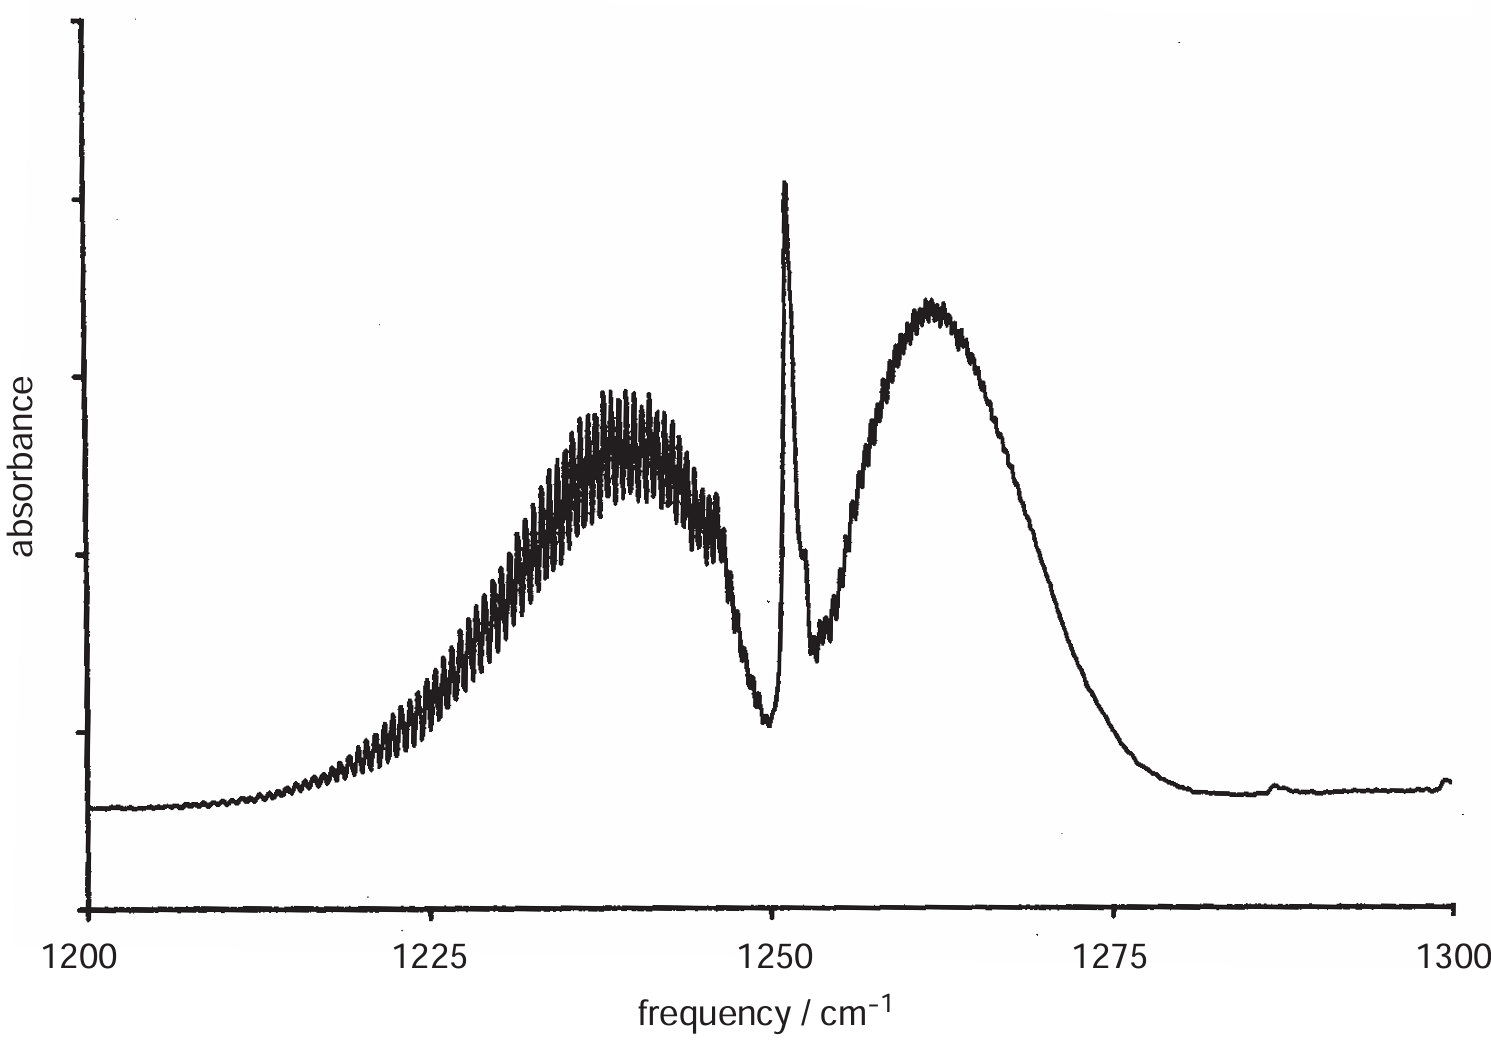
\includegraphics[width=0.55\textwidth]{CH3I_parallel.png}
        \caption{The spectrum of a parallel transition for \(\mathrm{CH_3I}\), adapted from Banwell. The partly resolved \(P\) and \(R\) branches are clearly visible, as is the intense \(Q\) branch.}
    \end{figure}

    The presence of centrifugal distortion terms alters this simple picture somewhat. The \(P\), \(Q\), and \(R\) branches now no longer fall on top of one another, but are very slightly displaced; as a result, the band takes on a more complex appearance. However, at modest resolution the separate \(P\), \(Q\), and \(R\) branches are often not resolved from one another and so the band
    appears to have a ``simple'' \(PQR\) structure.

    \subsubsection*{Perpendicular Transition}
    For perpendicular transitions the selection rules for the rotational quantum numbers are
    \begin{equation}
        \Delta J=0,\pm 1\quad \Delta K=\pm 1\,.
    \end{equation}
    For each value of \(K\) we thus expect there to be a \(P\), \(Q\), and \(R\) branch corresponding to \(\Delta K=+1\) and one for \(\Delta K=-1\).

    Assuming, for simplicity, that the rotational constants do not change with vibrational state, and ignoring centrifugal distortion, the frequencies of the \(P\), \(Q\), and \(R\) branch lines for a prolate top are
    \begin{align}
        \tilde{\nu}_P(J,K)&=\tilde{\omega}_0-2\tilde{B}_J+(\tilde{A}-\tilde{B})(1\pm 2K)\\
        \tilde{\nu}_Q(J,K)&=\tilde{\omega}_0+(\tilde{A}-\tilde{B})(1\pm 2K)\\
        \tilde{\nu}_R(J,K)&=\tilde{\omega}_0+2\tilde{B}(J+1)+(\tilde{A}-\tilde{B})(1\pm 2K)\,.
    \end{align}
    For each value of \(K\) there is a set of \(PQR\) branches centred at \(\tilde{\omega}_0+(\tilde{A}-\tilde{B})(1+ 2K)\) (corresponding to \(\Delta K=+1\)), and another set centred at \(\tilde{\omega}_0+(\tilde{A}-\tilde{B})(1- 2K)\) (corresponding to \(\Delta K=-1\)). Since \(\tilde{A}-\tilde{B}\) is usually comparable with the rotational constants, the displacement of these sets of \(PQR\) branches is easily resolved.

    There are so many of these \(PQR\) branches that the resulting spectrum is very complex indeed. Typically, in moderate resolution, the only features which are visible are the strong \(Q\) branches; the \(P\) and \(R\) branch lines are so numerous that they merge into one another. It is clear from the above that the separation of the \(Q\) branches is \(2(\tilde{A}-\tilde{B})\); provided that \(\tilde{B}\) is known (e.g. from a parallel transition), it is thus possible to determine \(\tilde{A}\). This is in contrast to the pure rotational spectrum from which it is not possible to determine \(\tilde{A}\).

    \begin{figure}
        \centering
        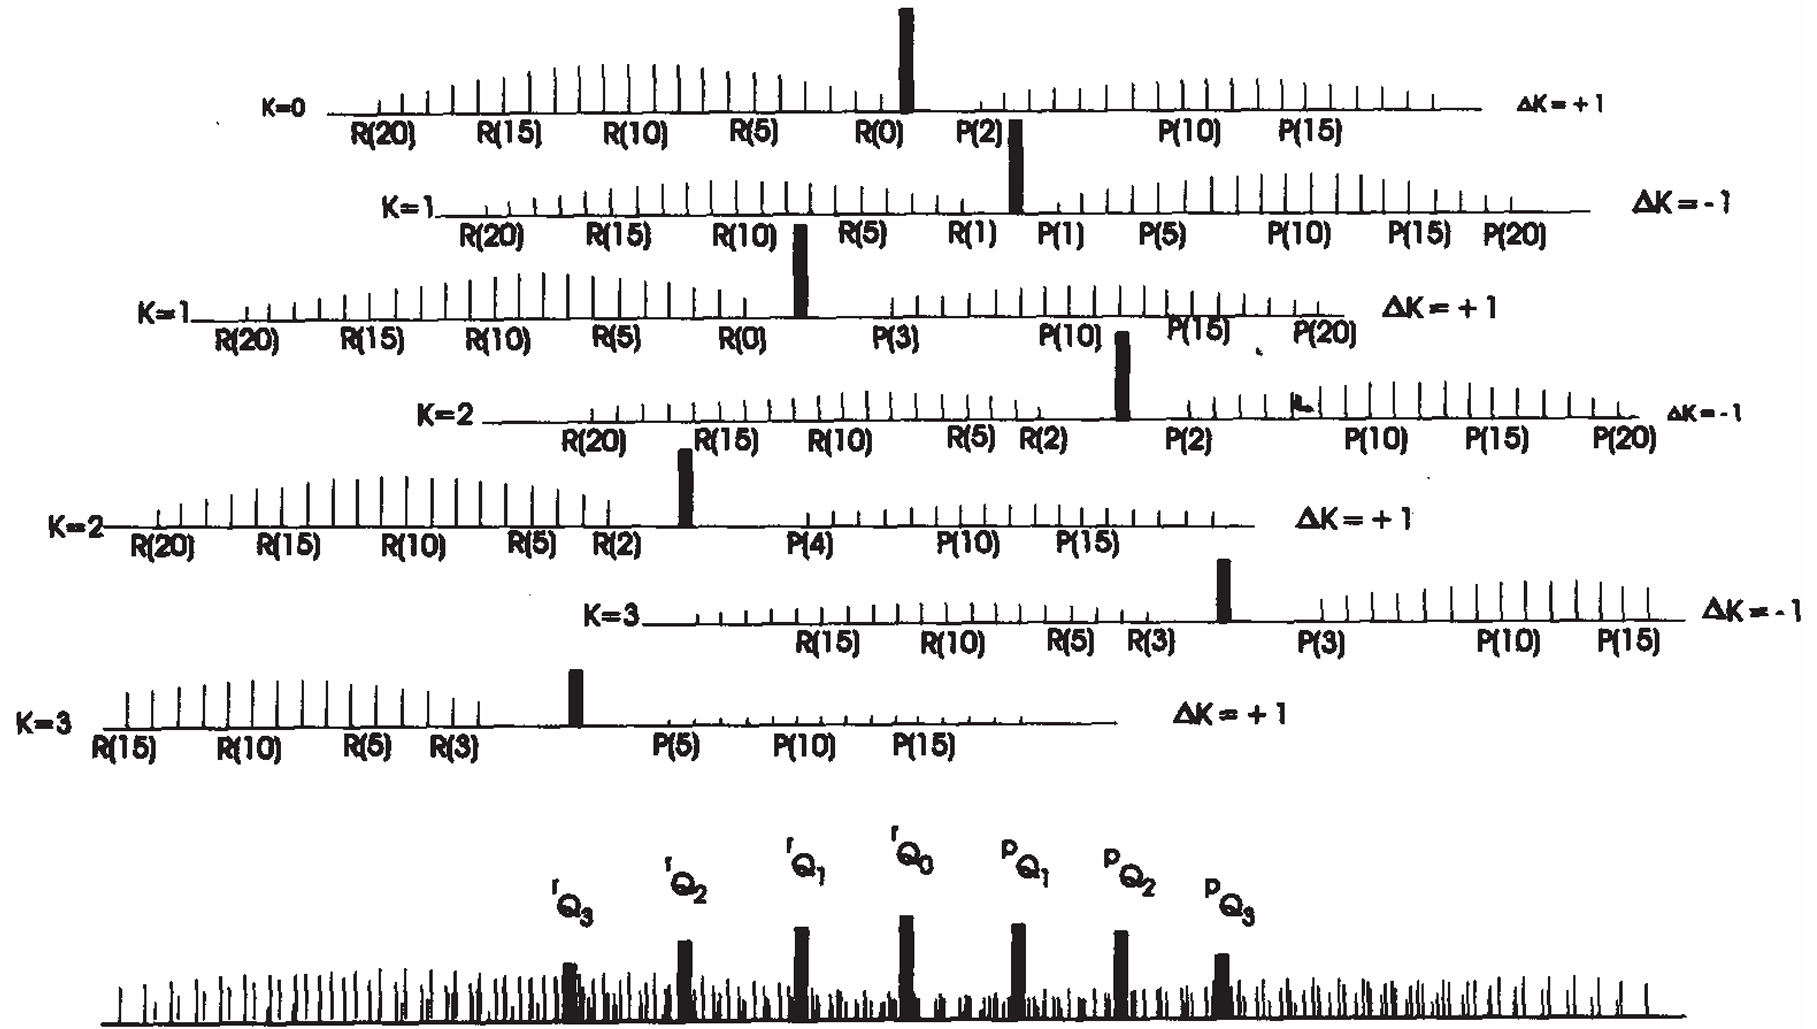
\includegraphics[width=0.92\textwidth]{prolate_top_perpendicular.png}
        \caption{A schematic spectrum for a perpendicular transition of a prolate top, adapted from Bernath. A perpendicular band is constructed from overlapping \(P\), \(Q\), and \(R\) branches from different \(K\) values and with \(\Delta K=\pm 1\). Note how the lines in the \(P\) and \(R\) branches form a forest of lines, leaving the narrow \(Q\) branches to stand out. (The notation used is that \(^rQ_K\) is the \(Q\) branch corresponding to the transition with \(\Delta K=+1\) for a given \(K\), and \(^pQ_K\) is the \(Q\) branch corresponding to the transition with \(\Delta K=-1\).)}
    \end{figure}

    \begin{figure}
        \centering
        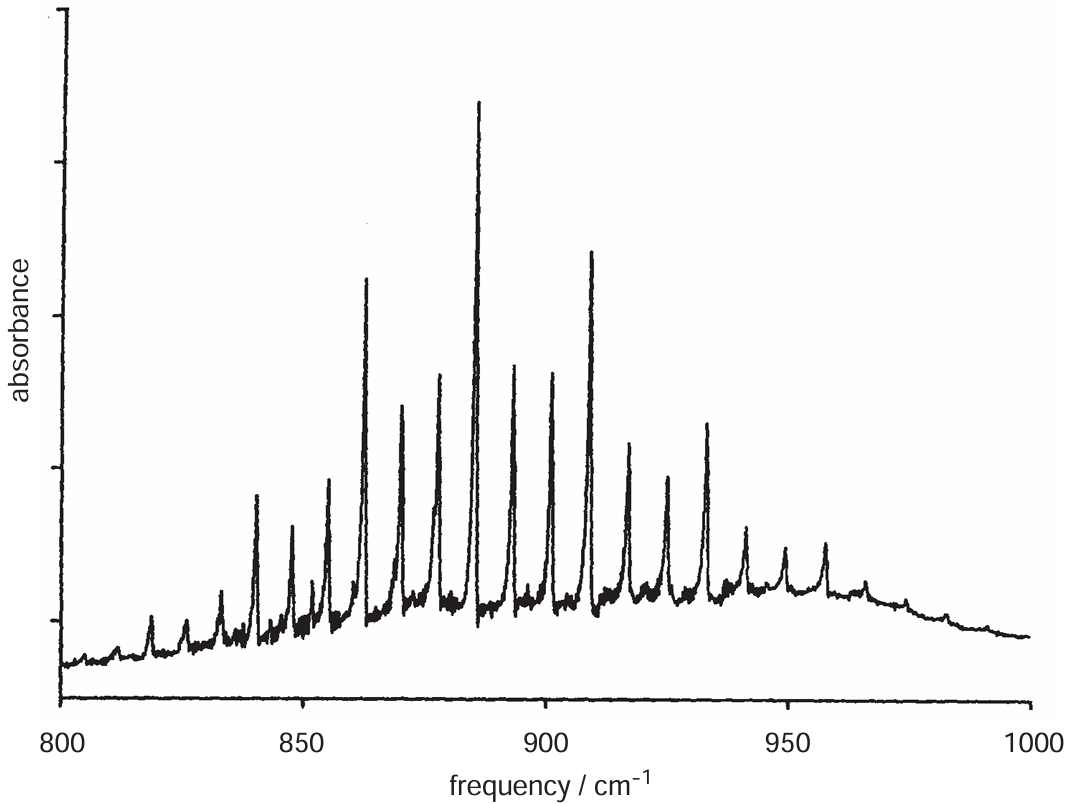
\includegraphics[width=0.55\textwidth]{CH3I_perpendicular.png}
        \caption{The spectrum of a perpendicular transition for \(\mathrm{CH_3I}\), adapted from Banwell. Only the intense \(Q\) branches are visible.}
    \end{figure}

    \subsubsection{Intensities}
    In the case of pure rotational transitions, it is necessary to take into account both stimulated absorption and stimulated emission in order to explain the observed intensities of the lines. However, in the case of rotational fine structure associated with a vibrational transition, the upper state (which involves a vibrational excitation) is hardly populated, so we usually only need consider stimulated absorption. The dominant factor determining the intensities of these rotational fine structure transitions is thus the populations of the ground states.

    \subsubsection{Nuclear Spin Effects}
    In the IB \textit{Molecular Energy Levels and Thermodynamics} course we described how, in symmetrical molecules, the intensities of rotational transitions are affected by nuclear spin. For example, we saw that in the fundamental of the asymmetric stretch of \(\mathrm{^{12}C ^{16}O_2}\), only lines originating from even \(J\) levels in the ground state are present.

    This discussion was limited to symmetrical linear molecules belonging to point group \(D_{\infty h}\). However, similar effects are seen in symmetric top molecules. For example, the \(Q\) branches seen in a perpendicular transition of \(\mathrm{C {^{1}H_3} F}\) show a \(2:1:1:2\) intensity alternation on account of the three equivalent hydrogen atoms whose nuclei have spin one half.

    \subsection{Direct Product}\label{Chap:direct_product}
    Below are the direct product tables for a selection of some commonly encountered point groups. Direct product is commutative, so only the upper half of the table is shown.
    \begin{table}[ht!]
        \centering
        \begin{tabular}{c|ccc}
            \toprule
            \(C_{3v},D_{3h}\) & \(A_1\) & \(A_2\) & \(E\) \\ \midrule
            \(A_1\) & \(A_1\) & \(A_2\) & \(E\) \\
            \(A_2\) & ~ & \(A_1\) & \(E\) \\
            \(E\) & ~ & ~ & \(A_1\oplus[A_2]\oplus E\) \\ \bottomrule
        \end{tabular}
    \end{table}
    \begin{table}[ht!]
        \centering
        \begin{tabular}{c|cccc}
            \toprule
            \(C_{\infty v}, D_{\infty h}\) & \(\Sigma^+\) & \(\Sigma^-\) & \(\Pi\) & \(\Delta\) \\ \midrule
            \(\Sigma^+\) & \(\Sigma^+\) & \(\Sigma^-\) & \(\Pi\) & \(\Delta\) \\
            \(\Sigma^-\) & ~ & \(\Sigma^+\) & \(\Pi\) & \(\Delta\) \\
            \(\Pi\) & ~ & ~ & \(\Sigma^+ \oplus[\Sigma^-]\oplus\Delta\) & \(\Pi\oplus\Phi\) \\
            \(\Delta\) & ~ & ~ & ~ & \(\Sigma^+ \oplus[\Sigma^-]\oplus\Gamma\) \\ \bottomrule
        \end{tabular}
    \end{table}

    For those with \('\) and \(''\), or \(g\) and \(u\) labels, the products are as follows.
    \begin{table}[ht!]
        \centering
        \hfill
        \begin{tabular}{c|cc}
            \toprule
            ~ & \('\) & \(''\) \\ \midrule
            \('\) & \('\) & \(''\) \\
            \(''\) & \(''\) & \('\) \\
            \bottomrule
        \end{tabular}
        \hfill
        \begin{tabular}{c|cc}
            \toprule
            ~ & \(g\) & \(u\) \\ \midrule
            \(g\) & \(g\) & \(u\) \\
            \(u\) & \(u\) & \(g\) \\
            \bottomrule
        \end{tabular}
        \hfill\(\,\)
    \end{table}

    \newpage

    \section{Raman Spectroscopy}
    In ``normal'' spectroscopy we look at the light which is either absorbed or emitted by a molecule. However, there are other processes by which a molecule can interact with radiation, such as \textit{scattering} which is the topic of this section. In a scattering experiment we shine a beam of monochromatic light through the sample and detect photons which emerge from the sample in all directions: these photons are said to be scattered. It is important to realize that these scattered photons do not arise from the original photons being absorbed and then re-emitted (that would be fluorescence/phosphorescence), but from a completely different process.

    Typically, only a tiny fraction of the incident photons are scattered so detecting them has in the past represented quite a challenge. However, the ready availability of lasers, which emit intense well-collimated beams of monochromatic light, have made such scattering experiments much easier to perform.

    The majority of scattered photons are at exactly the same frequency as the incoming photons from the laser: this type of scattering is called \textit{Rayleigh scattering}. However, it is found that some of the scattered photons have lower energy than the photons from the laser, and some have higher energy than the laser photons. This type of scattering in which there is a change in the photon energy is called \textit{Raman scattering}.
    
    The interpretation of Raman scattering is that in the scattering process the laser photon either loses energy as the scattering molecule moves up from one energy level to another, or gains energy as the molecule moves down from one energy level to another. The energy separation between the scattered photon and the laser photon therefore depends on the separation of the molecular energy levels, and so measurements of the energies of the scattered photons gives information about molecular energy levels, just in the same way as other forms of spectroscopy.

    \begin{figure}[ht!]
        \centering
        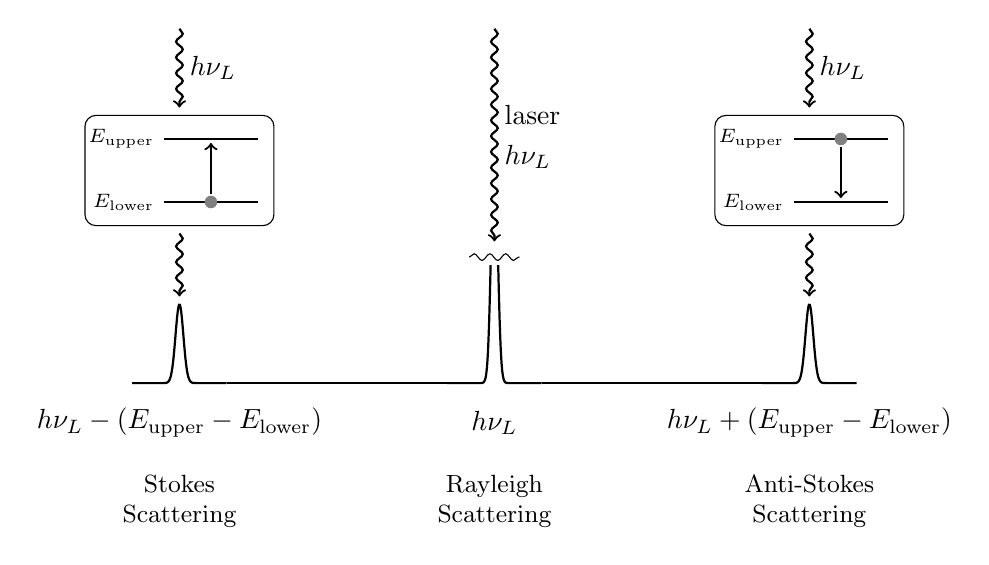
\begin{tikzpicture}
            \draw[thick,domain=-0.6:0.6, smooth, variable=\x,samples=100] plot ({\x}, {3*2.72^(-300*\x*\x)});
            \fill[white] (-1,1.5) rectangle (1,3.1);
            \draw[decoration = {snake,amplitude=1.2pt,segment length=2mm},decorate] (-0.32,1.6)--(0.32,1.6); 
            \draw[decoration = {snake,amplitude=1.2pt,segment length=2mm},decorate,->,thick] (0,4.5)--node[above right]{laser}node[below right]{\(h\nu_L\)}(0,1.8);
            \draw[thick,domain=-0.6:0.6, smooth, variable=\x,samples=100] plot ({\x-4}, {2.72^(-200*\x*\x)});
            \draw[thick,domain=-0.6:0.6, smooth, variable=\x,samples=100] plot ({\x+4}, {2.72^(-200*\x*\x)});
            \draw[thick] (-3.4,0)--(-0.6,0);
            \draw[thick] (3.4,0)--(0.6,0);
            \draw[rounded corners] (-5.2,2) rectangle (-2.8,3.4);
            \draw (-4.2,2.3)node[left]{\scriptsize\(E_{\text{lower}}\)}--(-3,2.3);
            \draw (-4.2,3.1)node[left]{\scriptsize\(E_{\text{upper}}\)}--(-3,3.1);
            \fill[gray] (-3.6,2.3) circle (0.08);
            \draw[thick,->] (-3.6,2.4)--(-3.6,3.05);
            \draw[decoration = {snake,amplitude=1.2pt,segment length=2mm},decorate,->,thick] (-4,4.5)--node[right]{\(h\nu_L\)}(-4,3.5);
            \draw[decoration = {snake,amplitude=1.2pt,segment length=2mm},decorate,->,thick] (-4,1.9)--(-4,1.1);
            \draw[rounded corners] (5.2,2) rectangle (2.8,3.4);
            \draw (3.8,2.3)node[left]{\scriptsize\(E_{\text{lower}}\)}--(5,2.3);
            \draw (3.8,3.1)node[left]{\scriptsize\(E_{\text{upper}}\)}--(5,3.1);
            \fill[gray] (4.4,3.1) circle (0.08);
            \draw[thick,<-] (4.4,2.35)--(4.4,3);
            \draw[decoration = {snake,amplitude=1.2pt,segment length=2mm},decorate,->,thick] (4,4.5)--node[right]{\(h\nu_L\)}(4,3.5);
            \draw[decoration = {snake,amplitude=1.2pt,segment length=2mm},decorate,->,thick] (4,1.9)--(4,1.1);
            \node at (0,-0.5) {\(h\nu_L\)};
            \node[align=center] at (0,-1.5) {\small Rayleigh\\[-1pt]\small Scattering};
            \node at (-4,-0.5) {\(h\nu_L-(E_{\text{upper}}-E_{\text{lower}})\)};
            \node[align=center] at (-4,-1.5) {\small Stokes \\[-1pt]\small Scattering};
            \node at (4,-0.5) {\(h\nu_L+(E_{\text{upper}}-E_{\text{lower}})\)};
            \node[align=center] at (4,-1.5) {\small Anti-Stokes \\[-1pt]\small Scattering};
        \end{tikzpicture}
    \end{figure}

    \subsection{Theory of Raman Scattering}
    An explanation of Raman scattering using quantum mechanics is not possible using the framework we have introduced so far. It is necessary to postulate the existence of ``virtual energy states'' which are created by the transient interaction between the molecule and the laser photon: these states are not the same as the normal energy levels of the molecule. The details of this approach are well beyond the level of this course, so we will not pursue it further.\footnote{An incomplete explanation using time-dependent perturbation theory can be found in C7: \textit{Further Quantum Mechanics}.} We can, however, develop a classical description of scattering which is helpful in interpreting the results of the full quantum mechanical analysis and which will provide us with a framework for understanding the Raman effect.

    \subsubsection{Classical Description}
    The key idea in this classical description is that the electric field of the laser light causes a distortion of the electron density of the molecule, resulting in the generation of an induced dipole.\footnote{The argument we present in this section is somewhat less handwaving than the one presented in the official handout.}
    
    The induced dipole fluctuates in sympathy with the oscillating electric field of the laser light. Classically, a fluctuating dipole generates radiation, and so this induced dipole results in radiation at the same frequency as the laser light: this is the origin of Rayleigh scattering. The size of the induced dipole depends on the \textit{polarisability} of the molecule: the more polarisable the molecule, the greater the distortion caused by a given electric field, the greater the induced dipole and hence the stronger the scattering.
    
    The polarisability is a rank-2 tensor --- it may either be \textit{isotropic} or \textit{anisotropic}. For example, in a diatomic molecule it is easier to polarize the electrons parallel to the internuclear axis than it is to polarize them perpendicular to the internuclear axis, so its polarisability is anisotropic.

    \begin{figure}[ht!]
        \centering
        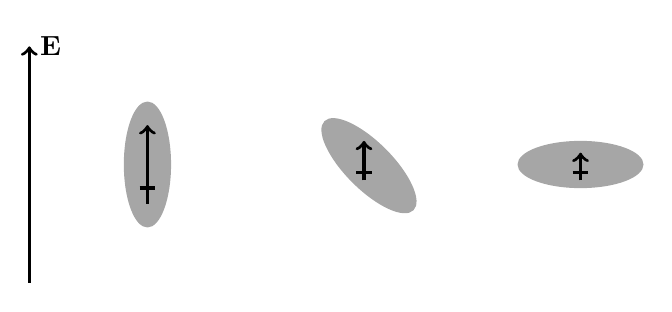
\begin{tikzpicture}
            \draw[very thick,->] (0,0)--(0,3)node[right]{\(\vb{E}\)};
            \fill[gray!70] (1.5,1.5) ellipse (0.3cm and 0.8 cm);
            \draw[very thick,->] (1.5,1)--(1.5,2);
            \draw[very thick] (1.4,1.2)--(1.6,1.2);
            \fill[gray!70,rotate=45] (4.1,-2) ellipse (0.3cm and 0.8 cm);
            \draw[very thick,->] (4.25,1.3)--(4.25,1.8);
            \draw[very thick] (4.15,1.4)--(4.35,1.4);
            \fill[gray!70] (7,1.5) ellipse (0.8cm and 0.3 cm);
            \draw[very thick,->] (7,1.3)--(7,1.65);
            \draw[very thick] (6.9,1.4)--(7.1,1.4);
        \end{tikzpicture}
        \caption{The polarisability of a diatomic molecule is anisotropic.}
    \end{figure}

    Assume the laser gives an oscillating electric field in the \(z\) direction
    \begin{equation}
        \vb{E}=E\sin(\omega_L t)\vu{z}\,.
    \end{equation}
    Let the polarisability of the molecule be the simple diagonal form
    \begin{equation}
        \alpha=\begin{pmatrix}
            \alpha_\perp & 0 & 0\\
            0 & \alpha_\perp & 0\\
            0 & 0 & \alpha_\parallel
        \end{pmatrix}\,,
    \end{equation}
    where \(\alpha_\perp<\alpha_\parallel\) accounting for the fact that the molecule is more polarisable along the internuclear axis.

    Now let the molecule rotate in the electric field. We will assume the molecule is rotating in the \(xz\) plane, and the internuclear axis is making an angle \(\theta\) with the direction of the electric field. The polarisability tensor is then 
    \begin{align}
        \alpha(\theta)&=\begin{pmatrix}
            \cos\theta & 0 & -\sin\theta \\
            0 & 1 & 0 \\
            \sin\theta & 0 & \cos\theta
        \end{pmatrix}\tp\begin{pmatrix}
            \alpha_\perp & 0 & 0\\
            0 & \alpha_\perp & 0\\
            0 & 0 & \alpha_\parallel
        \end{pmatrix}\begin{pmatrix}
            \cos\theta & 0 & -\sin\theta \\
            0 & 1 & 0 \\
            \sin\theta & 0 & \cos\theta
        \end{pmatrix}\notag\\
        &=\begin{pmatrix}
            \cos^2\theta\,\alpha_\perp+\sin^2\theta\,\alpha_\parallel & 0 & \sin\theta\cos\theta(\alpha_\parallel-\alpha_\perp) \\
            0 & \alpha_\perp & 0 \\
            \sin\theta\cos\theta(\alpha_\parallel-\alpha_\perp) & 0 & \cos^2\theta\,\alpha_\parallel+\sin^2\theta\,\alpha_\perp
        \end{pmatrix}\,.
    \end{align}
    Therefore, the induced dipole is
    \begin{align}
        \vb{\mu}&=\alpha(\theta)\vb{E}\notag\\
        &=\begin{pmatrix}
            \cos^2\theta\,\alpha_\perp+\sin^2\theta\,\alpha_\parallel & 0 & \sin\theta\cos\theta(\alpha_\parallel-\alpha_\perp) \\
            0 & \alpha_\perp & 0 \\
            \sin\theta\cos\theta(\alpha_\parallel-\alpha_\perp) & 0 & \cos^2\theta\,\alpha_\parallel+\sin^2\theta\,\alpha_\perp
        \end{pmatrix}\begin{pmatrix}
            0 \\ 0 \\ E\sin(\omega_L t)
        \end{pmatrix}\notag\\
        &=E\sin(\omega_L t)\begin{pmatrix}
            \sin\theta\cos\theta(\alpha_\parallel-\alpha_\perp) \\
            0 \\
            \cos^2\theta\,\alpha_\parallel+\sin^2\theta\,\alpha_\perp
        \end{pmatrix}\notag\\
        &=\frac{1}{2}(\alpha_\parallel+\alpha_\perp)E\sin(\omega_L t)\begin{pmatrix}
            0 \\ 0 \\ 1
        \end{pmatrix}+\frac{1}{2}(\alpha_{\parallel}-\alpha_{\perp}) E\sin(\omega_L t)\begin{pmatrix}
            \sin 2\theta \\ 0 \\ \cos 2\theta
        \end{pmatrix}\,.
    \end{align}
    This induced dipole has two components --- one aligned with the electric field of the laser, the other with lower magnitude rotating in the \(xz\) plane twice as fast as the molecule.\footnote{The official note directly stated the \(z\) component of this result, and ignored the \(x\) direction to avoid using tensors.}

    We now focus on the more interesting direction --- the \(z\) direction, since it has both components. Define
    \begin{equation}
        \alpha_{\text{av}}=\frac{1}{2}(\alpha_\parallel+\alpha_\perp)\qquad\Delta\alpha=\frac{1}{2}(\alpha_\parallel-\alpha_\perp)\,,
    \end{equation}
    and let \(\theta=\omega_R t\) i.e. the molecule is rotating at angular frequency \(\omega_R\). Then the induced dipole along the \(z\) axis is
    \begin{equation}
        \mu_z=\alpha_{\text{av}}E\sin(\omega_L t)+\Delta\alpha E\cos(2\omega_R t)\sin(\omega_L t)\,.
    \end{equation}
    The first term has the same frequency as the laser, so it gives rise to the Rayleigh scattering. The second term can be rewritten as
    \begin{equation}
        \frac{1}{2}\Delta\alpha E\left[\sin((\omega_L+2\omega_R)t)+\sin((\omega_L-2\omega_R)t)\right]\,.
    \end{equation}
    They are the Stokes and anti-Stokes scattering with frequencies \(2\omega_R\) higher and lower than the laser frequency. Note the amplitude of these terms is proportional to \(\alpha_\parallel-\alpha_\perp\), the anisotropy of the molecule's polarisability.

    In words, what is happening here is that the rotation of an anisotropic molecule leads to a \textit{modulation}, at the rotational frequency, in the size of the induced dipole, as is illustrated above. This variation of the dipole results in a corresponding variation in the amplitude of the radiation originating from the dipole. A sine wave which is modulated in amplitude by another sine wave has a Fourier transform in which there are additional components shifted from the original frequency by \(\pm\) the modulation frequency, as is illustrated in the figure.

    \begin{figure}
        \centering
        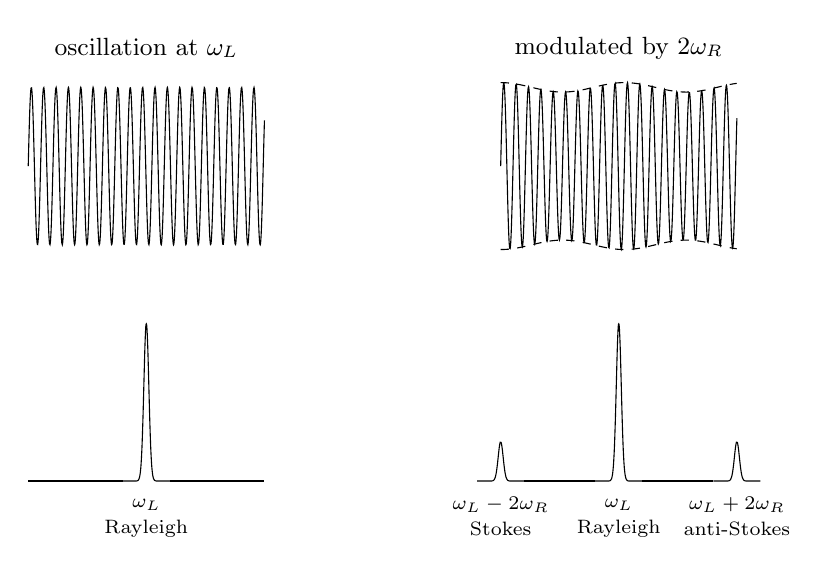
\begin{tikzpicture}
            \draw[domain=0:3, smooth, variable=\x,samples=500] plot ({\x}, {sin(40*\x r)});
            \draw[domain=0:3, smooth, variable=\x,samples=500] plot ({\x+6}, {(sin(40*\x r))*(1+0.06*cos(4*\x r))});
            \draw[dashed,domain=0:3, smooth, variable=\x,samples=300] plot ({\x+6}, {1+0.06*cos(4*\x r)});
            \draw[dashed,domain=0:3, smooth, variable=\x,samples=300] plot ({\x+6}, {-1-0.06*cos(4*\x r)});
            \node at (1.5,1.5) {\small oscillation at \(\omega_L\)};
            \node at (7.5,1.5) {\small modulated by \(2\omega_R\)};
            \draw[domain=-0.3:0.3, smooth, variable=\x,samples=50] plot ({\x+1.5}, {2*2.72^(-500*\x*\x)-4});
            \draw (0,-4)--(1.2,-4);
            \draw (1.8,-4)--(3,-4);
            \node at (1.5,-4.3) {\scriptsize\(\omega_L\)};
            \node at (1.5,-4.6) {\scriptsize Rayleigh};
            \draw[domain=-0.3:0.3, smooth, variable=\x,samples=50] plot ({\x+7.5}, {2*2.72^(-500*\x*\x)-4});
            \draw[domain=-0.3:0.3, smooth, variable=\x,samples=50] plot ({\x+6}, {0.5*2.72^(-500*\x*\x)-4});
            \draw[domain=-0.3:0.3, smooth, variable=\x,samples=50] plot ({\x+9}, {0.5*2.72^(-500*\x*\x)-4});
            \draw (6.3,-4)--(7.2,-4);
            \draw (7.8,-4)--(8.7,-4);
            \node at (7.5,-4.3) {\scriptsize\(\omega_L\)};
            \node at (7.5,-4.6) {\scriptsize Rayleigh};
            \node at (6,-4.3) {\scriptsize\(\omega_L-2\omega_R\)};
            \node at (6,-4.6) {\scriptsize Stokes};
            \node at (9,-4.3) {\scriptsize\(\omega_L+2\omega_R\)};
            \node at (9,-4.6) {\scriptsize anti-Stokes};
        \end{tikzpicture}
    \end{figure}

    Within the terms of this explanation, we see that all that is required for Raman scattering due to rotation is that the molecule has an anisotropic polarisability. Therefore, all diatomics (including homonuclear ones) give rise to rotational Raman scattering, as do all linear polyatomic molecules. This is in contrast to microwave spectroscopy where molecules belonging to the point group \(D_{\infty h}\) do not give rise to spectra.
    
    The vibration of a molecule leads to a change in the electron density and hence a change in the polarisability of the molecule. As a result, molecular vibrations also give rise to Raman scattering. As we shall see in more detail below, normal modes which are not infra-red active may nevertheless give rise to Raman scattering.

    \subsubsection{Quantum Description}
    As we stated before, the quantum mechanical description of Raman scattering is far beyond the scope of this course. We will only state some results of it.

    \begin{figure}[ht!]
        \centering
        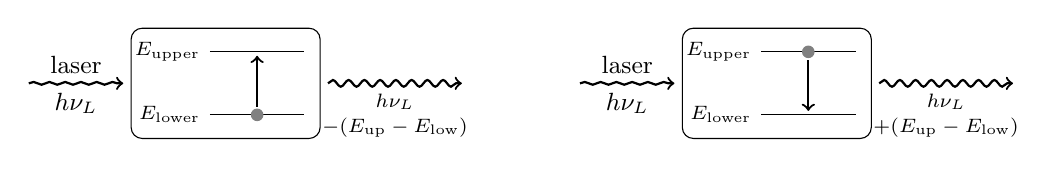
\begin{tikzpicture}
            \draw[rounded corners] (-4.2,2) rectangle (-1.8,3.4);
            \draw (-3.2,2.3)node[left]{\scriptsize\(E_{\text{lower}}\)}--(-2,2.3);
            \draw (-3.2,3.1)node[left]{\scriptsize\(E_{\text{upper}}\)}--(-2,3.1);
            \fill[gray] (-2.6,2.3) circle (0.08);
            \draw[thick,->] (-2.6,2.4)--(-2.6,3.05);
            \draw[->,decoration = {snake,amplitude=0.5pt,segment length=2mm},decorate,thick] (-5.5,2.7)--node[above]{\small laser}node[below]{\small \(h\nu_L\)}(-4.3,2.7);
            \draw[->,decoration = {snake,amplitude=1.2pt,segment length=2mm},decorate,thick] (-1.7,2.7)--node[below,align=center]{\scriptsize \(h\nu_L\) \\[-3pt] \scriptsize \(-(E_{\text{up}}-E_{\text{low}})\)}(0,2.7);
            \draw[rounded corners] (5.2,2) rectangle (2.8,3.4);
            \draw (3.8,2.3)node[left]{\scriptsize\(E_{\text{lower}}\)}--(5,2.3);
            \draw (3.8,3.1)node[left]{\scriptsize\(E_{\text{upper}}\)}--(5,3.1);
            \fill[gray] (4.4,3.1) circle (0.08);
            \draw[thick,<-] (4.4,2.35)--(4.4,3);
            \draw[->,decoration = {snake,amplitude=0.5pt,segment length=2mm},decorate,thick] (1.5,2.7)--node[above]{\small laser}node[below]{\small \(h\nu_L\)}(2.7,2.7);
            \draw[->,decoration = {snake,amplitude=1.2pt,segment length=2mm},decorate,thick] (5.3,2.7)--node[below,align=center]{\scriptsize \(h\nu_L\) \\[-3pt] \scriptsize \(+(E_{\text{up}}-E_{\text{low}})\)}(7,2.7);
        \end{tikzpicture}
    \end{figure}

    If in the scattering process the molecule moves from a lower energy level, with energy \(E_{\text{lower}}\), to a higher energy level \(E_{\text{upper}}\), the conservation of energy dictates that
    \begin{equation}
        h\nu_{\text{Stokes}}=h\nu_L-(E_{\text{upper}}-E_{\text{lower}})\,.
    \end{equation}
    Similarly, for a scattering process in which the molecule drops down from \(E_{\text{upper}}\) to \(E_{\text{lower}}\) we have
    \begin{equation}
        h\nu_{\text{anti-Stokes}}=h\nu_L+(E_{\text{upper}}-E_{\text{lower}})\,.
    \end{equation}
    The above equations can be easily rewritten in terms of wavenumbers
    \begin{equation}
        \tilde{\nu}=\tilde{\nu}_L\pm\abs{\Delta\tilde{\epsilon}}\,.
    \end{equation}

    Whether or not the scattering process is allowed for any particular pair of energy levels will depend on relevant selections rules, which are detailed below. The intensity of the scattering process depends on the polarisability of the molecule and the population of the energy level in which the molecule starts. At equilibrium, these populations will be determined by the Boltzmann distribution.

    We will also see that we recover the classical picture in the classical limit. If we substitute the quantum rotational energy levels into the above expression together with the selection rules (see later), we would expect the Stokes and anti-Stokes lines to appear at \(2\tilde{B}(2J+3)\) from the Rayleigh line, which can be approximated to \(4\tilde{B}J\) in the classical limit for \(J\gg 1\). Using the relation \(E=\hbar\omega\), this corresponds to a shift in photon angular frequency of
    \begin{equation}
        \Delta\omega=\frac{2\hbar J}{I}\,.
    \end{equation}
    Also in the classical limit, the molecule has angular momentum \(\norm{\vb{J}}=\hbar\sqrt{J(J+1)}\approx J\hbar\), which relates to the angular frequency \(\omega_R\) at which the molecule rotates by \(\norm{\vb{J}}=I\omega_R\). Hence we get
    \begin{equation}
        \omega_R=\frac{\norm{\vb{J}}}{I}=\frac{\hbar J}{I}\,.
    \end{equation}
    We obtained our classical relation \(\Delta\omega=2\omega_R\) i.e. the Stokes and anti-Stokes scattering have frequencies \(2\omega_R\) higher and lower than the laser frequency.

    \subsection{Experimental Raman Spectroscopy}
    The experimental arrangement for Raman spectroscopy is that an intense monochromatic beam of light is directed through the sample, the scattered radiation is then collected and its frequency analysed in the usual way by dispersing it with a prism or a diffraction grating, or analysing it using an interferometer (as in an FTIR experiment). The scattered light comes out in all directions, so it is advantageous to collect it from directions perpendicular to the exciting beam so as to minimize the amount of this intense light which reaches the detector.
    
    Laser light, on account of its high intensity, monochromaticity and high degree of collimation, is ideal for recording Raman spectra. Since the intensity of Raman scattering is very low, but proportional to the intensity of the exciting radiation, it is very advantageous to use an intense source. Any frequency spread in the source translates to a frequency spread in the scattered photons (i.e. a linewidth), so the monochromatic nature of laser light gives the highest resolution spectra. Finally, the collimation of the light means that it can be directed through the sample and, if necessary, passed back and forth many times so as to increase the number of scattered photons.
    
    It is important that the laser light is not absorbed directly by the molecules being studied as this would give rise to fluorescence which would swamp the much weaker signal due to Raman scattering. Photons from the visible region are easy to detect with high sensitivity, so this indicates using a laser in the visible region. However, this increases the chance that the laser light will be absorbed directly.
    
    In the past, it was common to use light at \(633\unit{nm}\) (red) from a He-Ne laser or at \(515\unit{nm}\) (green) from argon-ion laser. However, recent advances in the efficiency with which infra-red photons can be detected, along with the use of Fourier transform instruments for analysing the scattered light, have led to the use of \(1064\unit{nm}\) light (which is in the near infra-red) from the Nd-YAG laser. Such near infra-red light is far less likely to be absorbed by the molecules.

    \subsection{Rotational Raman Spectroscopy}
    Changes in rotational energy lead to Raman scattered light which is separated from the laser line by typical rotational energies i.e. a few \(\!\unit{cm}^{-1}\). Detecting such a weak signal close in to the very strong laser line is very challenging experimentally.

    \subsubsection{Diatomics and Linear Polyatomics}
    All such molecules have anisotropic polarisability so lead to Raman scattering. The selection rules are
    \begin{equation}
        \Delta J=0,\pm 2\,.
    \end{equation}
    Scattered photons with \(\Delta J=0\) have the same frequency as the laser line, so will not be separable from Rayleigh scattering.

    The labelling of the lines requires some care. Recall that:
    \begin{enumerate}[topsep=0pt,label=(\roman*)]
        \item \(\Delta J\) is defined as \((J_{\text{upper}}-J_{\text{lower}})\).
        \item lines are labelled according to the \(J\) value of the lower level.
    \end{enumerate}

    A Stokes scattering event in which the molecule starts from  \(J=0\) and ends in \(J=2\) will appear on the low frequency side of the laser line and will have \(\Delta J=J_{\text{upper}}-J_{\text{lower}}=2-0=+2\). An anti-Stokes scattering event in which the molecule starts from \(J=2\) and ends in \(J=0\) will appear on the high frequency side of the laser line. However, according to the definition above \(\Delta J=J_{\text{upper}}-J_{\text{lower}}=2-0=+2\). The lines are labelled with the \(J\) value of the lower level, which in this case \(0\) for both.

    Under typical conditions many rotational levels are occupied so we expect to see several lines corresponding to \(J=0,1,2,\dots\). The situation is therefore reminiscent of the (microwave) rotational spectrum.

    Let us first consider the Stokes lines, and assume that the rotational energy levels can be modelled using the rigid rotor, with levels
    \begin{equation}
        \tilde{E}_J=\tilde{B}J(J+1)\,.
    \end{equation}
    The wavenumber of the scattered photon is that of the laser minus the separation of the rotational levels, giving
    \begin{align}
        \tilde{\nu}_{\text{Stokes}}(J)&=\tilde{\nu}_L-[\tilde{E}_{J+2}-\tilde{E}_J]\notag\\
        &=\tilde{\nu}_L-2\tilde{B}(2J+3)\,.
    \end{align}
    We therefore see a series of lines at
    \begin{equation}
        \underbrace{\tilde{\nu}_L-6\tilde{B}}_{2\leftarrow 0}\,,\quad\underbrace{\tilde{\nu}_L-10\tilde{B}}_{3\leftarrow 1}\,,\quad\underbrace{\tilde{\nu}_L-14\tilde{B}}_{4\leftarrow 2}\dots
    \end{equation}
    Note that the first line is shifted (to lower wavenumber) by \(6\tilde{B}\) from the laser line and that subsequent lines are spaced by \(4\tilde{B}\).

    The anti-Stokes transitions are similar.
    \begin{align}
        \tilde{\nu}_{\text{anti-Stokes}}(J)&=\tilde{\nu}_L+[\tilde{E}_{J+2}-\tilde{E}_J]\notag\\
        &=\tilde{\nu}_L+2\tilde{B}(2J+3)\,.
    \end{align}
    The first line is shifted (to higher wavenumber) by \(6\tilde{B}\) from the laser line and subsequent lines are spaced by \(4\tilde{B}\).

    Since both Stokes and anti-Stokes transitions have \(\Delta J=+2\), they are both referred to as \(S\) branches. The Stokes line closest to the laser is therefore labelled \(S(0)\) and subsequent Stokes lines are labelled \(S(1),S(2),\dots\) Similarly, the anti-Stokes line closest to the laser is
    labelled \(S(0)\) and subsequent anti-Stokes lines are labelled \(S(1),S(2),\dots\)

    The intensities of these lines follow a contour similar to that for the microwave spectrum.
    \begin{figure}
        \centering
        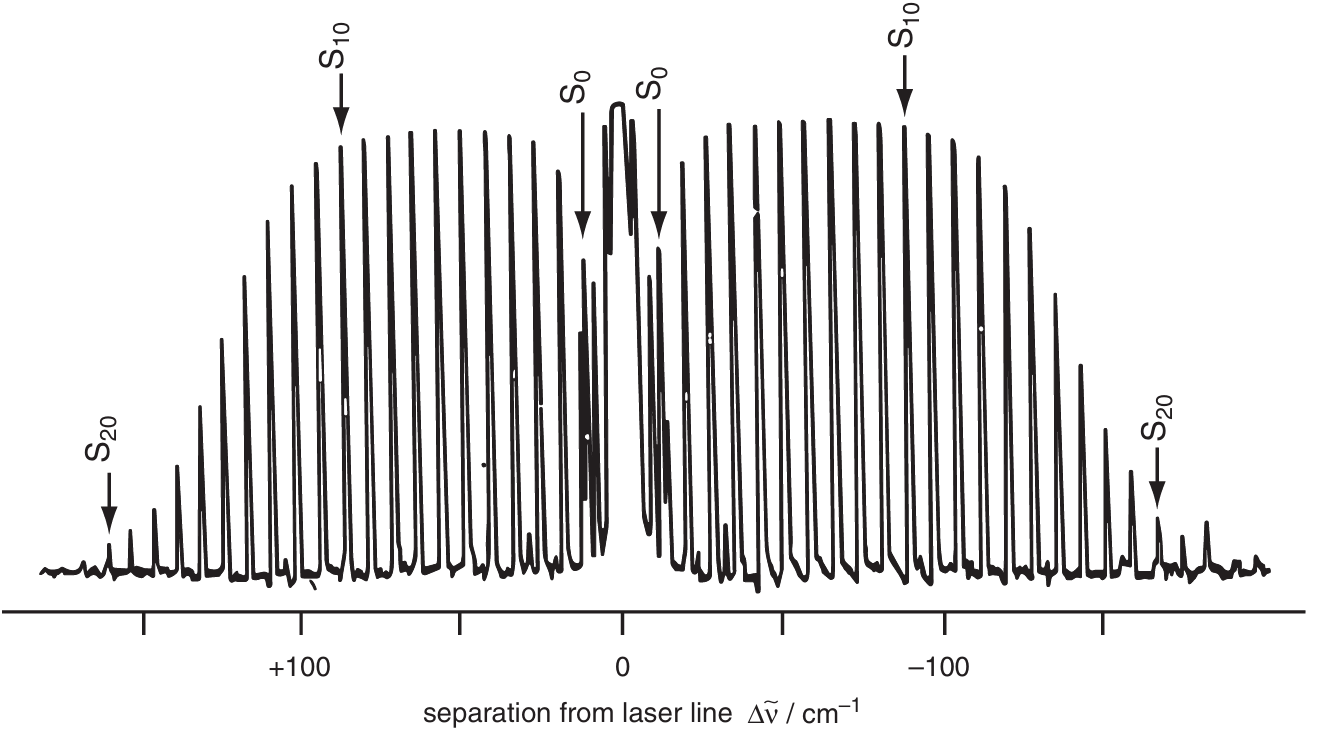
\includegraphics[width=0.7\textwidth]{rot_raman.png}
        \caption{The rotational Raman spectrum of \(\mathrm{^{15}N^{14}N}\), adapted from Hollas. Note that the intensities of the lines with low \(J\) values have been somewhat truncated by experimental effects.}
    \end{figure}
    \subsubsection{Symmetric Tops}
    All such molecules have an anisotropic polarisability so lead to Raman scattering. The selection rules are \(\Delta J=0,\pm 1,\pm 2\), \(\Delta K=0\). Transitions with \(\Delta J=\pm 1\) give lines shifted from the laser line by \(2\tilde{B},4\tilde{B},6\tilde{B},\dots\), and those with \(\Delta J=\pm 2\) give lines shifted from the laser line by \(6\tilde{B},10\tilde{B},14\tilde{B},\dots\)
    \subsubsection{Spherical Tops}
    Spherical tops have isotropic polarisabilities. They do not give rise to rotational Raman spectra.

    \subsection{Vibrational Raman Spectra}
    \subsubsection{Diatomics}
    The gross selection rule is that there must be a change in polarisability during the vibration. This is always the case, so all diatomics give rise to vibrational Raman spectra. The harmonic oscillator selection rule is \(\Delta v=\pm 1\), as in the infra-red.

    If we use the harmonic oscillator energy levels as a simple model, then a transition from \(v=0\) to \(v=1\) leads to a Raman line on the low frequency side of the laser line (Stokes scattering), with frequency
    \begin{equation}
        \tilde{\nu}_{\text{Stokes}}(1\leftarrow 0)=\tilde{\nu}_L-\tilde{\omega}\,.
    \end{equation}
    Similarly, a transition from \(v=1\) to \(v=0\) leads to an anti-Stokes line at
    \begin{equation}
        \tilde{\nu}_{\text{anti-Stokes}}(1\rightarrow 0)=\tilde{\nu}_L+\tilde{\omega}\,.
    \end{equation}
    Under typical conditions the \(v=1\) level is barely populated so the anti-Stokes line will be much weaker than the Stokes line.

    \subsubsection*{Rotational Fine Structure}
    As in the infra-red, a change in vibrational energy can be accompanied by a change in rotational energy. For vibrational Raman spectroscopy the selection rules for rotational levels are:
    \begin{equation}
        \Delta J=0,\pm 2\,.
    \end{equation}
    \(\Delta J=-2\) transitions will lead to an \(O\) branch and \(\Delta J=+2\) will lead to an \(S\) branch. Note that this fine structure is spread about the frequency of the vibrationally scattered line (e.g. about \(\tilde{\nu}_L-\tilde{\omega}\)) and not about the laser line. In addition, the \(\Delta J=0\) transitions form a \(Q\) branch, clustered at the centre. If we assume that the rotational levels can be described using a rigid rotor and that the rotational constant is independent of the vibrational state, then the frequencies of the Stokes scattered lines are
    \begin{align}
        \tilde{\nu}_O(J)&=\tilde{\nu}_L-[\tilde{\omega}-2\tilde{B}(2J-1)]\\
        \tilde{\nu}_Q(J)&=\tilde{\nu}_L-\tilde{\omega}\\
        \tilde{\nu}_S(J)&=\tilde{\nu}_L-[\tilde{\omega}+2\tilde{B}(2J+3)]
    \end{align}
    where \(\tilde{\omega}\) is the frequency of the pure vibrational transition. For the \(O\) branch \(J=2,3,\dots\) and for the \(Q\) and \(S\) branches \(J=0,1,\dots\). Note that, in this approximation, all of the lines in the \(Q\) branch fall on top of one another, and the spacing in the \(O\) and \(S\) branches is \(4\tilde{B}\).

    If we make the more realistic assumption that \(\tilde{B}\) varies with the vibrational state, then the lines in the \(Q\) branch are somewhat spread out, and the spacing in the other branches is no longer constant.  The values of the rotational constants can be found by using a modified version of the method of combination differences.

    \begin{figure}
        \centering
        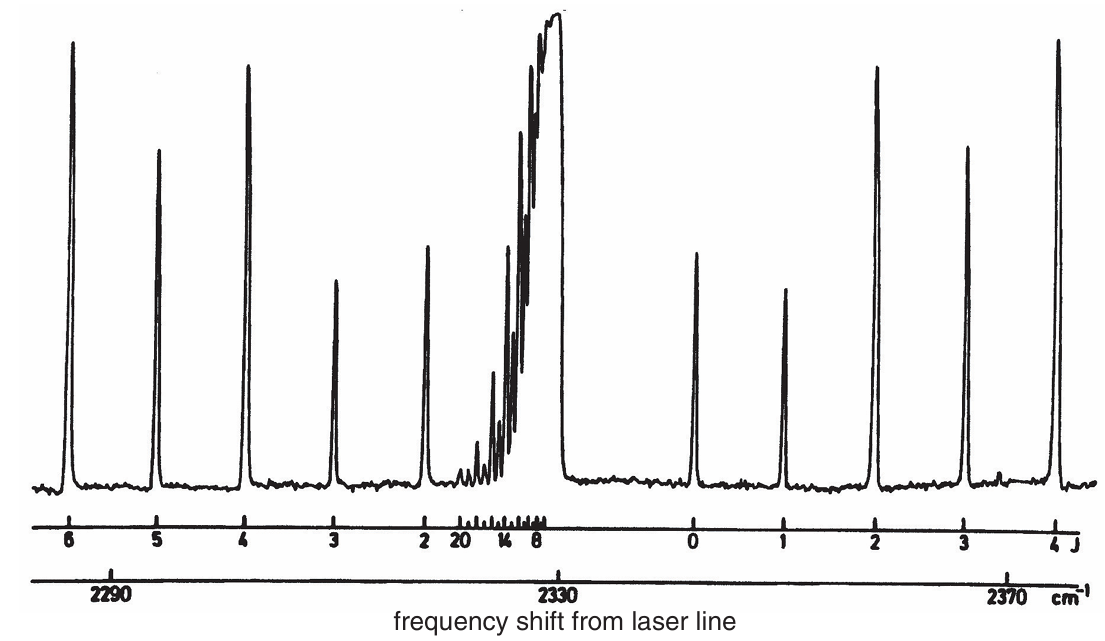
\includegraphics[width=0.75\textwidth]{vibrot_raman.png}
        \caption{The \(1\leftarrow 0\) vibrational transition in the Raman spectrum of \(\mathrm{^{14}N_2}\) (i.e. the Stokes peaks), adapted from Bernath. The intensity alternation is due to nuclear spin effects. Note that the horizontal scale is the shift in frequency from the laser line, and that all of these peaks are on the low frequency side of the laser. The \(O\) branch lines (left) appear at higher absolute frequencies than those in the \(S\) branch (right).}
    \end{figure}
    \subsubsection{Raman Activity of Normal Modes}
    The intensity of Raman scattering involving a transition between vibrational states \(i\) and \(j\) depends on the transition moment
    \begin{equation}
        R_{ij}=\int\dd{\tau}\psi_i^*\hat{\alpha}\psi_j\,.
    \end{equation}
    It will be non-zero only if the triple direct product
    \begin{equation}
        \Gamma_i\otimes\Gamma^\alpha\otimes\Gamma_j
    \end{equation}
    includes the totally symmetric irreducible representation.

    Following a similar line of argument as for the infra-red, we can easily show that the fundamental of a particular normal mode gives rise to Raman scattering if the IR of the normal mode matches that of \(x_ix_j\). Such a mode is said to be \textit{Raman active}. As before, symmetry arguments can be used to examine whether or not overtones or combination lines are Raman active.

    \subsubsection*{Rule of Mutual Exclusion}
    If a point group contains the centre of inversion \(i\) as a symmetry operation, then the character of \(x\), \(y\) and \(z\) under \(i\) must be \(-1\), as by definition, \(i\) does the transformation \((x,y,z)\mapsto(-x,-y,-z)\). The character of quadratic functions \(x_ix_j\) must be \(+1\) because \(x_ix_j\mapsto(-x_i)(-x_j)=x_ix_j\). Hence, \(x_i\) and \(x_i x_j\) must transform as different irreducible representations. Hence we get the rule of mutual exclusion.

    \fbox{\begin{minipage}{0.9\textwidth}
        In a centrosymmetric molecule, the fundamental of any normal mode cannot be infra-red active and Raman active at the same time.
    \end{minipage}}

    \subsubsection{Intensities and Polarisations}
    In non-centrosymmetric molecules it is rare for any of the modes to be Raman inactive. However, it is found that the strength of Raman scattering varies considerably from mode to mode. So-called \textit{breathing modes}, in which all of the bonds around a central atom stretch together, often give rise  to particularly strong Raman scattering. In contrast, bending modes give weak scattering.

    If the laser light used to excite Raman scattering is plane polarized, then it is found that some of scattered light is polarized in the same direction as the laser light (called the \textit{parallel component}) and some of the scattered light is polarized at right angles to the laser light (called the \textit{perpendicular component}). The ratio of the intensity of the perpendicular (\(I_\perp\)) to the parallel scattering (\(I_\parallel\)) is called the \textit{depolarization ratio} \(\rho\), defined as
    \begin{equation}
        \rho=\frac{I_\perp}{I_\parallel}\,.
    \end{equation}
    This ratio is easily measured using polarizing filters.

    The detailed theory of Raman scattering shows that \(0\le\rho\le\frac{3}{4}\). Scattering from totally symmetric modes, such as the breathing modes referred to above, tend to have depolarization ratios close to zero i.e. all the scattered light is polarized parallel to the laser light. The Raman bands from such modes are said to be \textit{polarized}.

    On the other hand, non-totally-symmetric modes often have depolarization ratios close to the theoretical maximum of \(3/4\). Such bands are said to be \textit{depolarized}. Measurements of \(\rho\) can therefore help to distinguish which normal mode is responsible for a particular band.

    \subsection{Applications of Raman Spectroscopy}
    Although it is technically more difficult than microwave or infra-red spectra, Raman spectroscopy is useful as it provides complementary information or, in some cases, information that is simply not obtainable by other forms of spectroscopy.
    \begin{enumerate}[topsep=0pt,label=(\roman*)]
        \item The vibrational and rotational energy levels of homonuclear diatomics, and the rotational levels of symmetrical linear polyatomics, can only be probed directly using Raman spectroscopy (but electronic spectra may give the same information).
        \item Vibrational Raman spectroscopy is complementary to infra-red when it comes to elucidating the vibrational normal modes: in centrosymmetric molecules, some normal modes may only be detectable using Raman spectroscopy.
        \item As Raman spectroscopy uses light which is scattered, rather than transmitted, the technique can be used for surface analysis, especially of solid materials.
    \end{enumerate}

    \newpage

    \section{Electronic Spectroscopy of Diatomics}
    In electronic spectroscopy absorptions occur due to transitions between electronic energy levels; typically these transitions occur in the visible or UV part of the spectrum. Electronic transitions are accompanied by simultaneous changes in vibrational and rotational energy leading to extensive fine structure and hence very complex spectra. As a result, only the electronic spectra of the simplest molecules are understood in detail. We will confine our discussion to diatomics.

    Electronic spectra give information about the electronic energy levels available to a molecule, and about the vibrational and rotational levels associated with these energy levels. Together, this information provides a very detailed picture of the bonding in a molecule, and in particular the way the bonding varies with internuclear distance i.e. the potential energy curve. Electronic spectra are used in the remote detection and measurement of molecules e.g. for studies of the atmosphere and of interstellar species.
    
    Before we discuss the electronic energy levels of diatomic molecules it is useful to remind ourselves about the electronic energy levels of atoms, as many of the concepts which we use for atoms have direct parallels in molecules.

    \subsection{Electronic Energy Levels of Atoms}
    \subsubsection{Orbitals and Energy Levels}
    We are very used to describing the electronic structure of an atom by giving the electronic configuration, in which we indicate which \textit{orbitals} are occupied e.g. for carbon the configuration is \(\mathrm{1s^2 2s^2 2p^2}\). It is very important to realize that this orbital description is just an approximation (albeit a very useful one) and that the orbitals are not the energy levels of the atom.

    An \textit{orbital} is a one-electron wavefunction which is found on the assumption that the electron experiences an average repulsion from all the other electrons. As a result, the energy of a given orbital depends on the details of which other orbitals are occupied. When we first learn about orbitals we are encouraged to think of them as a fixed “ladder” of energy levels into which we can slot the electrons. Useful though this picture is, it is incomplete as it does not recognise the fact that the orbitals change in energy as additional electrons are added, or the electrons are rearranged.

    At a basic level atomic spectra can be thought of as arising due to an electron moving from one orbital to another, but this approach must be used with caution because, as noted above, the orbital energies change as the electrons are rearranged. The more formally correct view is that the electronic levels (or states) of the atom are described by a multi-electron wavefunction \(\Psi_n(\vb{r}_1,\vb{r}_2,\dots)\) which depends on the coordinates \(\vb{r}_i\) (and spin) of all of the electrons. Associated with each of these multi-electron wavefunctions is a particular energy, \(E_n\), and it is between these energy levels that spectroscopic transitions occur.

    \begin{figure}[ht!]
        \centering
        \begin{tikzpicture}
            \draw (0,0)--(1.5,0);
            \draw (0,0.5)--(1.5,0.5);
            \draw (0,2)--(1.5,2);
            \draw (0,3)--(1.5,3);
            \draw (0,3.6)--(1.5,3.6);
            \draw (4.5,0)--(3,0);
            \draw (4.5,0.5)--(3,0.5);
            \draw (4.5,2)--(3,2);
            \draw (4.5,3)--(3,3);
            \draw (4.5,3.6)--(3,3.6);
            \draw[fill=black] (0.6,0) circle (0.06);
            \draw[fill=black] (0.9,0) circle (0.06);
            \draw[fill=black] (0.6,0.5) circle (0.06);
            \draw[fill=black] (0.9,0.5) circle (0.06);
            \draw[fill=black] (3.6,0) circle (0.06);
            \draw[fill=black] (3.9,0) circle (0.06);
            \draw[fill=black] (3.6,0.5) circle (0.06);
            \draw[fill=black] (3.9,3) circle (0.06);
            \draw[very thick,->] (1.8,1.8)--(2.7,1.8);
            \node at (-1,1.8) {\small orbitals};
            \node at (2.25,-0.5) {\small approximate};

            \draw[very thick] (7,0)node[left]{\small\(\Psi_i\)}--(8.5,0);
            \draw (7,1)--(8.5,1);
            \draw (7,1.8)--(8.5,1.8);
            \draw (7,2.7)--(8.5,2.7);
            \draw (7,3.1)--(8.5,3.1);
            \draw (7,3.6)--(8.5,3.6);
            \draw (11.5,0)--(10,0);
            \draw (11.5,1)--(10,1);
            \draw[very thick] (11.5,1.8)node[right]{\small\(\Psi_f\)}--(10,1.8);
            \draw (11.5,2.7)--(10,2.7);
            \draw (11.5,3.1)--(10,3.1);
            \draw (11.5,3.6)--(10,3.6);
            \draw[very thick,->] (8.8,1.8)--(9.7,1.8);
            \node at (6,1.8) {\small levels};
            \node at (9.25,-0.5) {\small exact};
        \end{tikzpicture}
    \end{figure}

    As a result of electron-electron repulsion there is no simple way of calculating the energies of either the orbitals or the multi-electron wavefunctions. Modern computer calculations can, however, give reliable estimations on energies and wavefunctions. Although we cannot determine these by hand we can say something about the wavefunctions which arise from a particular electronic configuration. In particular, we can specify the total spin and orbital angular momenta, which turn out to be very useful quantities to know when it comes to understanding the spectrum. Traditionally the values of these angular momenta (as quantum numbers) are collected together in a term symbol which is associated with an energy level.

    \subsubsection{Atomic Term Symbols}
    The method of obtaining atomic term symbols is explained in Part IB \textit{Introduction to Quantum Mechanics}. Here is a quick recap.

    Suppose that we have two sources of angular momentum, with quantum numbers \(j_1\) and \(j_2\). The total angular momentum of the system is  characterized by a quantum number \(J\) whose values are given by the Clebsch--Gordan series
    \begin{equation}
        J=j_1+j_2,j_1+j_2-1,\dots,\abs{j_1-j_2}\,.
    \end{equation}

    Using the Clebsch--Gordan series, we can work out the values of total spin quantum number \(S\) and total orbital angular momentum quantum number \(L\). These are combined in a \textit{term symbol}
    \begin{equation}
        ^{2S+1}L\,.
    \end{equation}
    Note the superscript is the \textit{spin degeneracy} \(2S+1\), not \(S\). The value of \(L\) is represented by a capital letter, with \(L\) values of \(0,1,2,3,\dots\) being indicated by the letters \(S,P,D,F,\dots\). It is also common to add a subscript to the term symbol indicating the value of \(J\), the total angular momentum, found by combining \(L\) and \(S\) using the Clebsch---Gordan series. However, here we are not interested in this quantum number and so will not discuss it further.

    Note a certain electron configuration may result in multiple possible terms. All of these will have different energies on account of how their different combinations of orbital and spin angular momentum affect the electron-electron repulsion. Hund's first rule indicates that the state with the lowest energy has the largest \(S\), and the second rule indicates that having maximised \(S\), the lowest energy state has maximum \(L\).

    For equivalent electrons the need to obey the Pauli principle means that certain term symbols arising for non-equivalent electrons are not permitted for equivalent electrons. The details of how this all works out in practice are beyond the scope of this discussion.

    \subsection{Molecular Term Symbols for Diatomics}
    Again, most of the content should be familiar from Part IB \textit{Symmetry and Bonding}. We will do a quick recap.

    An atom is spherical, so no direction is preferred over any other, and this means that the vector which represents the orbital angular momentum can point in any direction. If an electric or magnetic field is applied to the atom, then the direction of the field is distinct from all others and, as a consequence, we find that the vector which represents \(\ell\) can no longer point in any direction. Rather, \(\ell\) has to lie on a cone about the field direction, aligned such that the projection of \(\ell\) onto the field is \(m_\ell\), where \(m_\ell\) takes the values \(-\ell,\dots,\ell\) in integer steps.  This is the familiar phenomenon of space quantisation, and the direction along which the quantisation occurs is called the \textit{quantisation axis}.

    A linear molecule has such a distinct preferred direction on its own, in the absence of an external field; that is, the internuclear axis. As a result, in a diatomic we can specify the component of the angular momentum along the internuclear axis; this component is given the symbol \(\lambda\). In fact, so strong is the effect of this quantisation axis that it is really only possible to specify the angular momentum along this axis.
   
    For a \(\sigma\)-type MO the angular momentum along the internuclear axis is \(\lambda =0\). For a \(\pi\)-type MO, \(\lambda=\pm 1\), and for a \(\delta\)-type MO, \(\lambda=\pm 2\) and so on. These two values correspond to the two degenerate MOs.

    However, it is important to realize that the value of \(\lambda\) gives the projection onto the internuclear axis, and so this quantum number represents a scalar, not a vector. Therefore, when combining the angular momentum from two electrons we simply add the \(\lambda\) values numerically rather than adding them vectorially using the Clebsch--Gordan series.

    A molecular term symbol takes the form
    \begin{equation}
        ^{2S+1}\Lambda^{+/-}_{g/u}\,.
    \end{equation}
    \(2S+1\) is the spin multiplicity as before, and \(\Lambda\) is a capital Greek letter for the total angular momentum, where \(\Lambda=0,1,2,\dots\) are represented by \(\Sigma,\Pi,\Delta,\dots\).

    If the molecule belongs to the point group \(D_{\infty h}\), then a \(g\) or \(u\) is added by working out the overall symmetry of the state using the following rules
    \begin{equation}
        g\otimes g=g\quad u\otimes u=g\quad g\otimes u=u\,.
    \end{equation}
    For \(\Sigma\) states only, a superscript \(+/-\) is added to indicate the symmetry under reflection in a plane containing the internuclear axis.

    Most of the term symbols of diatomics are straightforward to work out as long as you keep in mind that full shells can be ignored and a hole is equivalent to an electron. An exception is the \(\pi^2\) configuration, which is the ground state of \(\mathrm{O}_2\). This is elaborated in the IB Symmetry and Bonding.

    Direct product provides a convenient way of determining the term symbol. Take the configuration \(\dots(1\pi_g^2)\) as an example. Using the direct product table,
    \begin{equation}
        \Pi_g\otimes\Pi_g=\Sigma_g^+\oplus[\Sigma_g^-]\oplus\Delta_g\,,
    \end{equation}
    where the antisymmetrised direct product is in the square bracket.

    Recall that Pauli exclusion principle requires the overall wavefunction, when the spatial and spin parts are included, be anti-symmetric with respect to exchange of electrons. Therefore, the spin triplet, which is spin symmetric, has to go with the anti-symmetric spatial function, which is \(\Sigma_g^-\). The spin singlet, which is spin anti-symmetric, can go with either of the symmetric spatial functions, \(\Sigma_g^+\) and \(\Delta_g\). Hence the possible term symbols are \(^1\Sigma_g^+\), \(^3\Sigma_g^-\) and \(^1\Delta_g\), with \(^3\Sigma_g^-\) being the ground state by Hund's first rule.

    \subsection{Potential Energy Curves}
    The energy of a particular electronic state is found to vary as the internuclear distance \(r\) changes. At some distance, called the \textit{equilibrium distance} or \textit{equilibrium bond length}, the energy goes to a minimum. As the distance decreases below this value the energy increases, usually rather steeply, on account of the unfavourable interactions between filled AOs. As the distance increases the energy rises as the overlap between AOs is less effective, eventually flattening out at large distances where we essentially have two non-interacting atoms i.e. dissociation. The resulting plot of energy vs distance \(r\) is called the \textit{potential energy curve} (PE curve). Each electronic state has such a PE curve associated with it.

    It is traditional to illustrate the electronic states of a molecule by plotting the PE curves for the various electronic states, as is illustrated here for \(\mathrm{C_2}\). The exact form of the PE curves and their energies has been inferred from a very detailed analysis of the spectra of this molecule.

    \begin{figure}
        \centering
        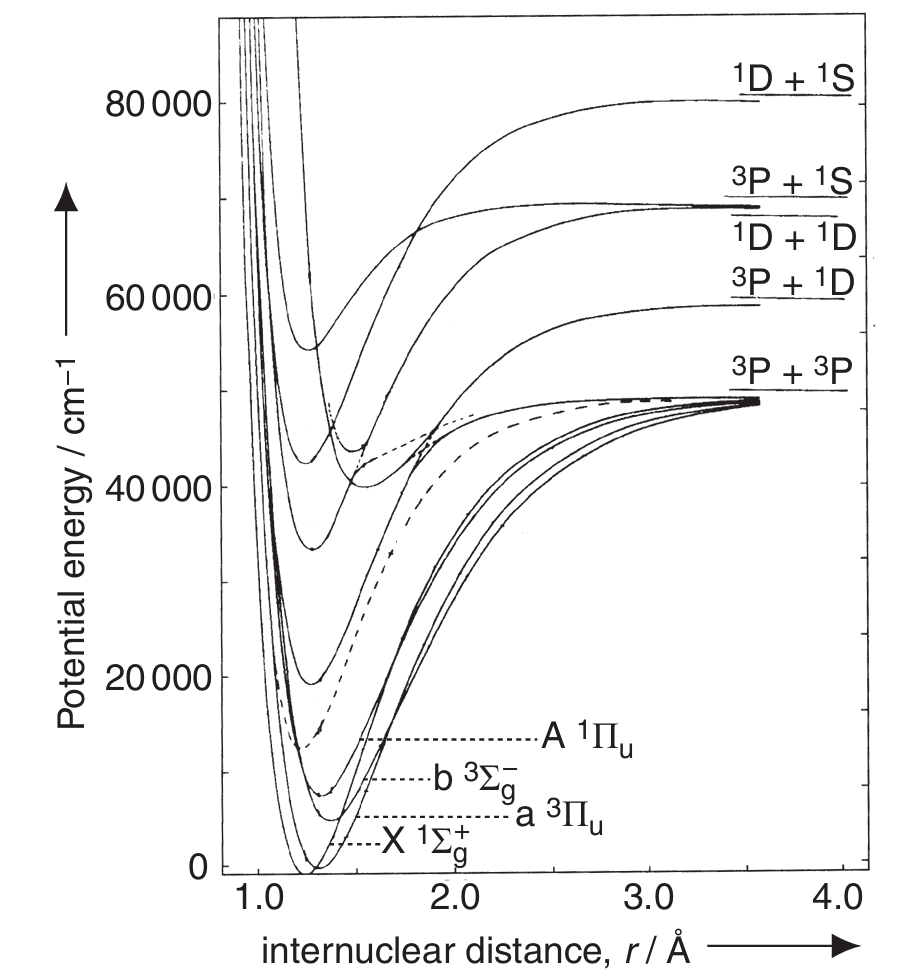
\includegraphics[width=0.5\textwidth]{PE_curve.png}
        \caption{The PE curves for the \(\mathrm{C_2}\) molecule. Figure adapted from Bernath.}
    \end{figure}

    A few remarks.
    \begin{enumerate}[topsep=0pt,label=(\roman*)]
        \item Even for this simple molecule, many excited electronic states have been identified, each with a unique PE curve: for each state the equilibrium bond length and the shape of the curve are different.
        \item Some of the electronic states of \(\mathrm{C_2}\) dissociate to give ground-state carbon atoms (term symbol \(^3P\)), but others dissociate to give carbon atoms in various excited states.
        \item  Some of the PE curves cross one another.
    \end{enumerate}

    It is also possible to have potential energy curves which have no minimum, but in which the energy simply falls as the internuclear distance increases. Such curves are said to be \textit{repulsive}. A molecule in such an electronic state will not be bound, but will simply dissociate into atoms.

    It is erroneous to call these PE curves ``Morse curves''. The Morse potential is just the simplest example of a function which has the same general shape as a typical PE curve. However, it turns out that the actual shape of these curves, especially at large internuclear distances, is only poorly approximated by the Morse potential.

    Each PE curve is labelled with the term symbol of the associated electronic state, prefixed with a letter to indicate the energy ordering of the states. The ground-state is denoted \(X\), and subsequent excited states with the same multiplicity (i.e. same value of \(S\)) as the ground state are denoted \(A,B,C\) etc. States with different multiplicity from the ground state are denoted by lower case letters in alphabetic sequence \(a,b,c\) etc. Unfortunately, this lettering convention is not the only one in use, so be prepared to be flexible.

    \subsubsection{Vibrational and Rotational Energy Levels in an Electronic State}
    Our discussion of spectroscopy rests on the Born--Oppenheimer separation in which we assume that the energy of a molecule can be separated into contributions from rotation, vibration and electronic motion. The justification for this is that the electrons are moving faster than either vibrations or rotations. The electrons rearrange themselves very quickly the moment the nuclei move in a rotation or vibration.

    As a result, we can associate with each potential energy curve a set of vibrational energy levels. The form of these levels depends on the precise shape of the PE curve. However, from our knowledge of the behaviour of the energy levels associated with the Morse potential we can reasonably expect that the levels will get closer together as the energy increases, and that at the dissociation limit these levels will become continuous.

    \begin{figure}[ht!]
        \centering
        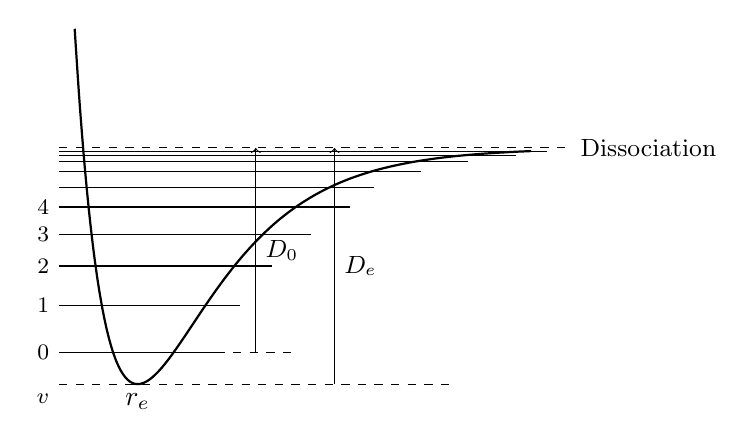
\begin{tikzpicture}
            \draw[thick,domain=-0.4:2.5, smooth, variable=\x,samples=100] plot ({2*\x}, {3*(1-2.72^(-2*\x))^2});
            \draw (-1,0.4)node[left]{\footnotesize \(0\)}--(1,0.4);
            \draw (-1,1)node[left]{\footnotesize \(1\)}--(1.3,1);
            \draw (-1,1.5)node[left]{\footnotesize \(2\)}--(1.7,1.5);
            \draw (-1,1.9)node[left]{\footnotesize \(3\)}--(2.2,1.9);
            \draw (-1,2.25)node[left]{\footnotesize \(4\)}--(2.7,2.25);
            \draw (-1,2.5)--(3,2.5);
            \draw (-1,2.7)--(3.6,2.7);
            \draw (-1,2.83)--(4.2,2.83);
            \draw (-1,2.9)--(4.8,2.9);
            \draw (-1,2.95)--(5.2,2.95);
            \draw[dashed] (-1,3)--(5.5,3)node[right]{\small Dissociation};
            \draw[dashed] (-1,0)node[below left]{\footnotesize \(v\)}--(4,0);
            \node at (0,0)[below]{\(r_e\)};
            \draw[dashed] (1,0.4)--(2,0.4);
            \draw[->] (2.5,0)--node[right]{\small \(D_e\)}(2.5,3);
            \draw[->] (1.5,0.4)--node[right]{\small \(D_0\)}(1.5,3);
        \end{tikzpicture}
    \end{figure}

    Generally, the energies of the vibrational levels can be written as a power series
    \begin{equation}
        \tilde{E}_v=\left(v+\frac{1}{2}\right)\tilde{\omega}_e-\left(v+\frac{1}{2}\right)^2\tilde{\omega}_e x_e+\left(v+\frac{1}{2}\right)^3\tilde{\omega}_e y_e +\dots\,,
    \end{equation}
    where \(\tilde{\omega}_e\) is the vibrational frequency and \(x_e,y_e,\dots\) are a series of dimensionless anharmonicity constants. For the harmonic oscillator only the first term is needed, and for the Morse oscillator only the first two terms are needed. In this latter case the depth of the potential energy curve \(\tilde{D}_e\) is given by
    \begin{equation}
        \tilde{D}_e=\frac{\tilde{\omega}_e}{4x_e}\,,
    \end{equation}
    and the dissociation energy is
    \begin{equation}
        \tilde{D}_0=\tilde{D}_e-\tilde{E}_0\,.
    \end{equation}
    It is important to realize that each electronic state has a different value for the vibrational frequency \(\tilde{\omega}_e\), the various anharmonicity constants and the dissociation energy. The values of these parameters are determined by the detailed shape of the PE curve.

    To further add to the complications, each vibrational level in each electronic state has associated with it a set of rotational energy levels. These can, for example, be modelled using the rigid rotor levels
    \begin{equation}
        \tilde{E}_J=\tilde{B}_{\text{elec},v}J(J+1)\,,
    \end{equation}
    where the rotational constant is a function of both the electronic state and the vibrational level. The variation of the rotational constant with vibrational state is quite small (\(\sim 1\%\)), but the equilibrium bond lengths of different electronic states can differ substantially, leading to a significant variation in the rotational constant between different electronic states. We shall shortly see the consequences of this.
    \subsection{Selection Rules}
    The selection rules for electronic transitions are
    \begin{equation}
        \Delta S=0\qquad\Delta\Lambda=0,\pm 1\notag
    \end{equation}
    \begin{equation}
        +\leftrightarrow +\quad -\leftrightarrow -\quad +\nleftrightarrow - \qquad\qquad g\leftrightarrow u\quad g\nleftrightarrow g \quad u\nleftrightarrow u\,.
    \end{equation}
    The spin selection rule \(\Delta S=0\) means that the ground state labelled \(X\) is only allowed to transition to excited states labelled with the upper case letters (\(A,B,C,\dots\)). If heavy atoms are present the spin selection rule starts to break down. For example, in \(\mathrm{I_2}\) the spin-forbidden transition \(^3\Pi\leftarrow ^1\Sigma\) is responsible for the purple colour of iodine vapour.

    There is no selection rule for the change in vibrational energy although, as we shall see shortly, the intensity of vibrational transitions varies quite markedly. For rotational transitions the rules are
    \begin{align}
        \text{For \(\Sigma\leftrightarrow\Sigma\) transitions: }&\Delta J=\pm 1\\
        \text{For \(\Sigma\leftrightarrow\Pi\) transitions: }&\Delta J=0,\pm 1
    \end{align}
    Therefore we expect to see \(P\) and \(R\) branches for \(\Sigma\leftrightarrow\Sigma\) transitions, and \(P,Q,R\) branches for \(\Sigma\leftrightarrow\Pi\) transitions.

    You can see how electronic spectra can become very complicated. Each electronic transition is accompanied by a number of different vibrational transitions. Then, each of these vibrational transitions has a \(P\), \(R\) and possibly \(Q\) branch fine structure associated with it. There is no reason to assume that the \(P/Q/R\) branches from different changes in vibrational levels will not overlap with one another: hence the spectrum becomes very complicated indeed.

    \subsubsection{Derivation of the Selection Rules using Symmetry}
    Recall that for a transition to be allowed, that is for the transition moment to be non-zero, the triple direct product
    \begin{equation}
        \Gamma_i\otimes\Gamma^\mu\otimes\Gamma_j
    \end{equation}
    must contain the totally symmetric irreducible representation.

    First we will consider heteronuclear diatomics, point group \(C_{\infty v}\), for which the \(z\) transforms as \(\Sigma^+\) and \((x,y)\) as \(\Pi\). Hence, the transition is allowed when either of the following two direct products contains \(\Gamma^{\text{tot.sym.}}\)
    \begin{equation}
        \begin{cases}
            \Gamma_i\otimes\Sigma^+\otimes\Gamma_j\\
            \Gamma_i\otimes\Pi\otimes\Gamma_j\\
        \end{cases}\,.
    \end{equation}
    This requires \(\Gamma_i\otimes\Gamma_j\) to contain either \(\Sigma^+\) or \(\Pi\).

    \begin{table}[ht!]
        \centering
        \begin{tabular}{c|cccc}
            \toprule
            \(C_{\infty v}, D_{\infty h}\) & \(\Sigma^+\) & \(\Sigma^-\) & \(\Pi\) & \(\Delta\) \\ \midrule
            \(\Sigma^+\) & \(\Sigma^+\) & \(\Sigma^-\) & \(\Pi\) & \(\Delta\) \\
            \(\Sigma^-\) & ~ & \(\Sigma^+\) & \(\Pi\) & \(\Delta\) \\
            \(\Pi\) & ~ & ~ & \(\Sigma^+ \oplus[\Sigma^-]\oplus\Delta\) & \(\Pi\oplus\Phi\) \\
            \(\Delta\) & ~ & ~ & ~ & \(\Sigma^+ \oplus[\Sigma^-]\oplus\Gamma\) \\ \bottomrule
        \end{tabular}
    \end{table}

    It is easy to observe from the direct product table that \(\Gamma_i\otimes\Gamma_j\) contains \(\Sigma^+\) if and only if \(\Gamma_i=\Gamma_j\), so here comes the selection rule \(\Delta\Lambda=0\) with the extra condition \(+\nleftrightarrow -\) to exclude \(\Sigma^+\otimes\Sigma^-=\Sigma^-\).

    The other possibility is for \(\Gamma_i\otimes\Gamma_j\) to contain \(\Pi\), which happens when \(\Sigma\otimes\Pi\), \(\Pi\otimes\Delta\) etc. i.e. \(\Delta\Lambda=\pm 1\).

    All these considerations apply to both hetero- and homonuclear diatomics. However, in the latter case we also need to consider the \(g/u\) symmetry label. It is obvious that in \(D_{\infty h}\), \(x,y,z\) all have the symmetry label \(u\) since the operation \(i\) is by definition the mapping \((x,y,z)\mapsto(-x,-y,-z)\). The totally symmetric irreducible representation has \(g\) symmetry, so it is evident that for the \(\Gamma_i\otimes\Gamma_j\) must have a \(u\) symmetry. This happens when the transition is \(u\leftrightarrow g\).

    \subsubsection{Absorption and Emission Spectra}
    Under normal conditions it is almost always the case that excited electronic states are too high in energy to be significantly populated. Therefore, absorption spectra are usually the result of transitions between the ground electronic state and various excited electronic states. In addition, it is likely that only the \(v''=0\) vibrational level within the ground electronic state is populated. Absorption spectra are therefore dominated by transitions from this level.

    Excited electronic states can be populated by passing a discharge through the gas, or perhaps creating the molecules in a high energy environment such as a flame. Emission spectra arising from transitions from these populated states to lower energy electronic states can then be observed. High vibrational states of the excited electronic states may also be populated in discharges, and transitions from these vibrational states may be seen. However, collisions between the molecules tend to degrade the vibrational energy, so it is often the case that the \(v'=0\) level is the most populated in an excited electronic state.

    \subsection{Vibrational Coarse Structure}
    To simplify things, we will temporarily ignore the rotational contribution to energy and just concentrate on the fine structure due to changes in vibrational energy. In addition, we will model the vibrational energy levels using Morse oscillators.

    Consider a transition (in absorption) from a vibrational level with quantum number \(v''\) in the lower electronic state to one with quantum number \(v'\) in the upper electronic state. Let \(T_e\) be the electronic energy measured at the bottom of the PE curve. Then the vibrational-electronic energy of the lower and upper levels are
    \begin{align}
        \tilde{E}_{v''}&=\tilde{T}_e''+\left(v''+\frac{1}{2}\right)\tilde{\omega}_e''-\left(v''+\frac{1}{2}\right)^2\tilde{\omega}_e''x_e''\\
        \tilde{E}_{v'}&=\tilde{T}_e'+\left(v'+\frac{1}{2}\right)\tilde{\omega}_e'-\left(v'+\frac{1}{2}\right)^2\tilde{\omega}_e'x_e'\,.
    \end{align}
    The transition occurs at
    \begin{equation}
        \tilde{\nu}_{v''v'}=\tilde{E}_{v'}-\tilde{E}_{v''}\,.
    \end{equation}

    The diagram below depicts such a electronic transition, along with various other parameters relating to the two potential energy curves. On the left it is assumed that the upper and lower electronic states dissociate to different atomic states: the energy separation between the atomic states is \(\Delta \tilde{E}_{\text{atomic}}\). The transition between the \(v=0\) level of the lower electronic state and the \(v=0\) level of the upper state, \(\tilde{\nu}_{00}\), is also shown, as are the dissociation energies and well depths (\(\tilde{D}_0\) and \(\tilde{D}_e\)) of the two PE curves. \(\tilde{\nu}_{\text{lim}}\) is the highest wavenumber (frequency) transition possible between the two states, going from \(v''=0\) to the dissociation limit of the upper state. On the right the two states are shown as dissociating to the same atomic levels: this diagram can be annotated in the same way.

    \begin{figure}[ht!]
        \centering
        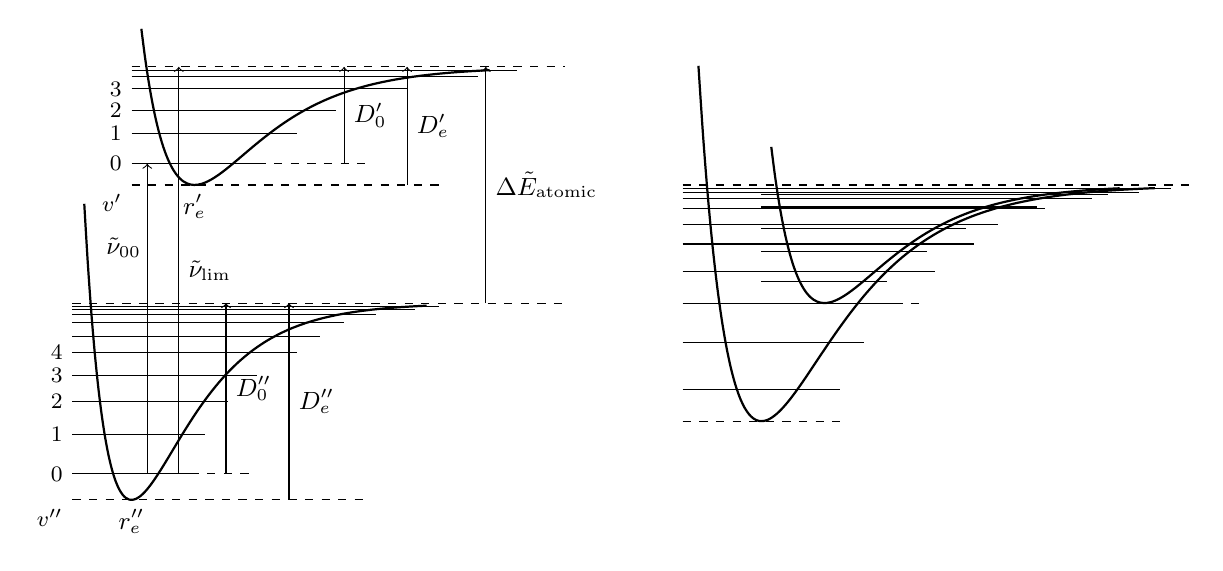
\begin{tikzpicture}
            \draw[thick,domain=-0.4:2.5, smooth, variable=\x,samples=100] plot ({1.5*\x}, {2.5*(1-2.72^(-2*\x))^2});
            \draw (-0.75,0.33)node[left]{\footnotesize \(0\)}--(0.75,0.33);
            \draw (-0.75,0.83)node[left]{\footnotesize \(1\)}--(0.93,0.83);
            \draw (-0.75,1.25)node[left]{\footnotesize \(2\)}--(1.23,1.25);
            \draw (-0.75,1.58)node[left]{\footnotesize \(3\)}--(1.6,1.58);
            \draw (-0.75,1.87)node[left]{\footnotesize \(4\)}--(2.1,1.87);
            \draw (-0.75,2.08)--(2.4,2.08);
            \draw (-0.75,2.25)--(2.7,2.25);
            \draw (-0.75,2.36)--(3.1,2.36);
            \draw (-0.75,2.42)--(3.6,2.42);
            \draw (-0.75,2.46)--(3.9,2.46);
            \draw[dashed] (-0.75,2.5)--(5.5,2.5);
            \draw[dashed] (-0.75,0)node[below left]{\footnotesize \(v''\)}--(3,0);
            \node at (0,0)[below]{\small\(r_e''\)};
            \draw[dashed] (0.75,0.33)--(1.5,0.33);
            \draw[->] (2,0)--node[right]{\small \(D_e''\)}(2,2.5);
            \draw[->] (1.2,0.33)--node[right]{\small \(D_0''\)}(1.2,2.5);

            \draw[thick,domain=-0.45:2.5, smooth, variable=\x,samples=100] plot ({1.5*\x+0.8}, {4+1.5*(1-2.72^(-1.7*\x))^2});
            \draw (0,4.27)node[left]{\footnotesize \(0\)}--(1.6,4.27);
            \draw (0,4.65)node[left]{\footnotesize \(1\)}--(2.1,4.65);
            \draw (0,4.95)node[left]{\footnotesize \(2\)}--(2.6,4.95);
            \draw (0,5.22)node[left]{\footnotesize \(3\)}--(3.5,5.22);
            \draw (0,5.38)--(4.4,5.38);
            \draw (0,5.45)--(4.9,5.45);
            \draw[dashed] (0,5.5)--(5.5,5.5);
            \draw[dashed] (0,4)node[below left]{\footnotesize \(v'\)}--(4,4);
            \node at (0.8,4)[below]{\small \(r_e'\)};
            \draw[dashed] (1.6,4.27)--(3,4.27);
            \draw[->] (3.5,4)--node[right]{\small \(D_e'\)}(3.5,5.5);
            \draw[->] (2.7,4.27)--node[right]{\small \(D_0'\)}(2.7,5.5);
            \draw[->] (0.2,0.33)--(0.2,4.27);
            \node at (-0.1,3.2) {\small \(\tilde{\nu}_{00}\)};
            \draw[->] (0.6,0.33)--node[right]{\small \(\tilde{\nu}_{\text{lim}}\)}(0.6,5.5);
            \draw[->] (4.5,2.5)--node[right]{\small \(\Delta\tilde{E}_{\text{atomic}}\)}(4.5,5.5);

            \draw[thick,domain=-0.4:2.5, smooth, variable=\x,samples=100] plot ({2*\x+8}, {1+3*(1-2.72^(-2*\x))^2});
            \draw (7,1.4)--(9,1.4);
            \draw (7,2)--(9.3,2);
            \draw (7,2.5)--(9.7,2.5);
            \draw (7,2.9)--(10.2,2.9);
            \draw (7,3.25)--(10.7,3.25);
            \draw (7,3.5)--(11,3.5);
            \draw (7,3.7)--(11.6,3.7);
            \draw (7,3.83)--(12.2,3.83);
            \draw (7,3.9)--(12.8,3.9);
            \draw (7,3.95)--(13.2,3.95);
            \draw[dashed] (7,4)--(13.5,4);
            \draw[dashed] (7,1)--(9,1);

            \draw[thick,domain=-0.45:2.5, smooth, variable=\x,samples=100] plot ({1.5*\x+8.8}, {2.5+1.5*(1-2.72^(-1.7*\x))^2});
            \draw (8,2.77)--(9.6,2.77);
            \draw (8,3.15)--(10.1,3.15);
            \draw (8,3.45)--(10.6,3.45);
            \draw (8,3.72)--(11.5,3.72);
            \draw (8,3.88)--(12.4,3.88);
            \draw (8,3.95)--(12.9,3.95);
            \draw[dashed] (8,2.5)--(10,2.5);
        \end{tikzpicture}
        \caption{Parameters for a transition between two electronic levels.}
    \end{figure}

    \subsubsection{Progressions and Sequences}
    A \textit{progression} is a series of transitions which share a common energy level. In an absorption spectrum, the separation between successive lines in a particular progression will reflect the spacing of the energy levels in the upper state. Therefore, the lines will get closer and closer together.

    A \textit{sequence} is a series of transitions which have a common value of \(\Delta v=v'-v''\). The more different the PE curves are, the more spread out the lines in the sequence are.

    \begin{figure}[ht!]
        \centering
        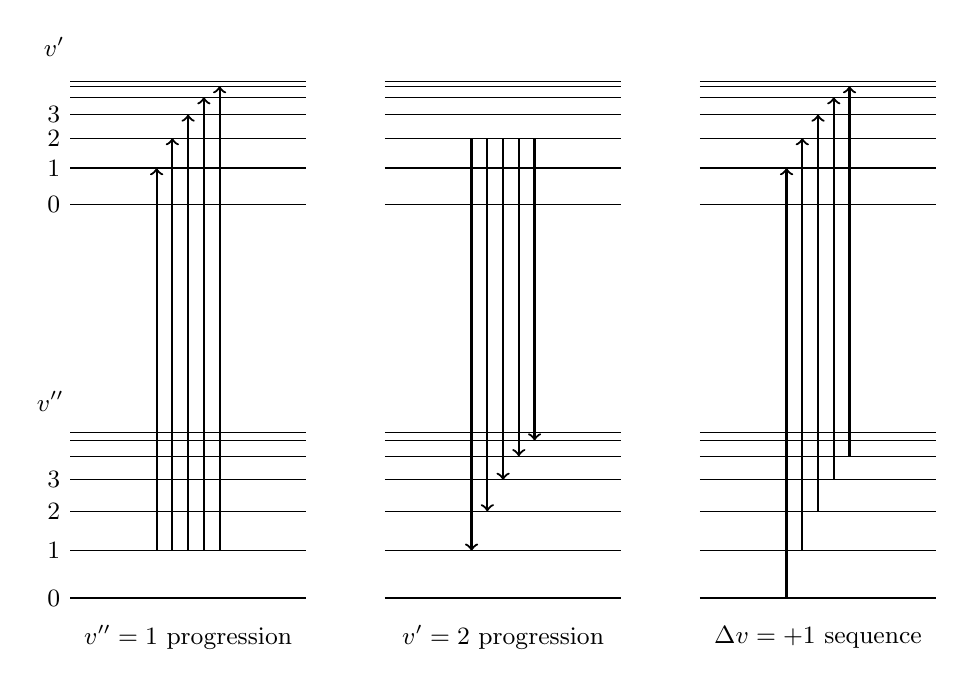
\begin{tikzpicture}
            \foreach \i in {0,...,3}{
                \draw (0,0.65*\i-0.05*\i*\i)node[left]{\small \(\i\)}--(3,0.65*\i-0.05*\i*\i);
            }
            \foreach \i in {4,5,6}{
                \draw (0,0.65*\i-0.05*\i*\i)--(3,0.65*\i-0.05*\i*\i);
            }
            \foreach \i in {0,...,6}{
                \draw (4,0.65*\i-0.05*\i*\i)--(7,0.65*\i-0.05*\i*\i);
                \draw (8,0.65*\i-0.05*\i*\i)--(11,0.65*\i-0.05*\i*\i);
            }
            \node at (-0.25,2.5){\small \(v''\)};
            \foreach \i in {0,...,3}{
                \draw (0,5+0.5*\i-0.04*\i*\i)node[left]{\small \(\i\)}--(3,5+0.5*\i-0.04*\i*\i);
            }
            \foreach \i in {4,5,6}{
                \draw (0,5+0.5*\i-0.04*\i*\i)--(3,5+0.5*\i-0.04*\i*\i);
            }
            \foreach \i in {0,...,6}{
                \draw (4,5+0.5*\i-0.04*\i*\i)--(7,5+0.5*\i-0.04*\i*\i);
                \draw (8,5+0.5*\i-0.04*\i*\i)--(11,5+0.5*\i-0.04*\i*\i);
            }
            \node at (-0.2,7){\small \(v'\)};
            \foreach \i in {1,...,5}{
                \draw[thick,->] (0.9+0.2*\i,0.6)--(0.9+0.2*\i,5+0.5*\i-0.04*\i*\i);
                \draw[thick,<-] (4.9+0.2*\i,0.65*\i-0.05*\i*\i)--(4.9+0.2*\i,5.84);
                \draw[thick,->] (8.9+0.2*\i,-0.7+0.75*\i-0.05*\i*\i)--(8.9+0.2*\i,5+0.5*\i-0.04*\i*\i);
            }
            \node at (1.5,-0.5){\small \(v''=1\) progression};
            \node at (5.5,-0.5){\small \(v'=2\) progression};
            \node at (9.5,-0.5){\small \(\Delta v=+1\) sequence};
        \end{tikzpicture}
    \end{figure}

    \subsubsection{Vibrational Intensities and Franck--Condon Factors}
    The intensity of a particular transition between levels \(i\) and \(j\) depends on the population of the lower level \(i\) and the modulus square of the transition moment
    \begin{equation}
        R_{ij}=\int\dd{\tau}\psi_i^*\hat{\mu}\psi_j\,.
    \end{equation}
    Using the Born--Oppenheimer separation, the wavefunctions can be written as a product of a wavefunction which depends only on the electrons \(\psi_{\text{el}}\) and a wavefunction which depends only on the vibrational motion of the nuclei \(\psi_{\text{vib}}\). We can also separate the dipole moment operator to a part acting on the vibrational wavefunction, and another part acting on the electronic wavefunction.
    \begin{align}
        R_{ij}&=\mel{\psi'_{\text{el}}}{\hat{\mu}_{\text{el}}}{\psi''_{\text{el}}}\braket{\psi_{\text{vib},i}}{\psi_{\text{vib},j}}+\mel{\psi_{\text{vib},i}}{\hat{\mu}_{\text{vib}}}{\psi_{\text{vib},j}}\cancel{\braket{\psi'_{\text{el}}}{\psi''_{\text{el}}}}\notag\\
        &=\mel{\psi'_{\text{el}}}{\hat{\mu}_{\text{el}}}{\psi''_{\text{el}}}\braket{\psi_{\text{vib},i}}{\psi_{\text{vib},j}}\,.
    \end{align}
    The inner product of two electronic wavefunctions is zero by orthogonality. \(R_{ij}\) factors out into two terms.

    The first term
    \begin{equation}
        \mel{\psi'_{\text{el}}}{\hat{\mu}_{\text{el}}}{\psi''_{\text{el}}}
    \end{equation}
    is the electronic transition moment, whose value is determined by the electronic states. If the transition is forbidden, this integral will be zero as we analysed in previous sections using symmetry.

    The second term is the overlap integral between the vibrational wavefunctions of the two electronic states. They are not orthogonal as they belong to different electronic states so they are not the eigenfunctions of the same Hermitian operator. The modulus square of this quantity is known as the \textit{Franck--Condon factor}
    \begin{equation}
        q_{ij}=\abs{\int\dd{\tau}\psi_{\text{vib},i}^*\psi_{\text{vib},j}}^2\,,
    \end{equation}
    and it is important in determining the intensity of transitions between different vibrational energy levels.

    As has already been discussed, absorption spectra almost always arise as a result of transitions from the ground vibrational level of the ground electronic state. We will therefore concentrate on transitions from this vibrational level.

    \begin{figure}
        \centering
        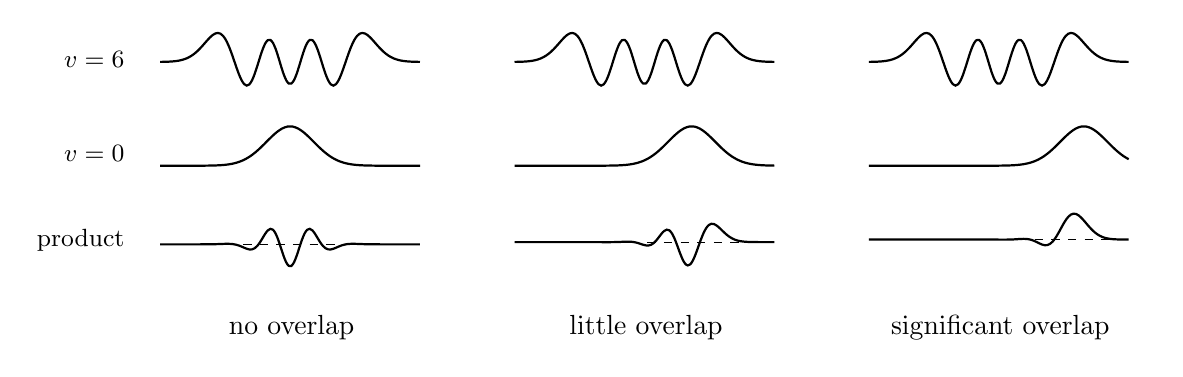
\begin{tikzpicture}
            \newcommand{\harmsix}{\begin{axis}[axis line style={draw=none},
                tick style={draw=none},yticklabels=\empty,xticklabels=\empty,x=0.3cm, y=0.5cm]
                \addplot [domain=-5.5:5.5, samples=100,thick,smooth]{(-120+720*x^2-480*x^4+64*x^6)*2.718^(-0.5*x^2)/(46080)^0.5};
            \end{axis}}
            \begin{scope}[shift={(0,3)}]
                \harmsix
            \end{scope}
            \begin{scope}[shift={(4.5,3)}]
                \harmsix
            \end{scope}
            \begin{scope}[shift={(9,3)}]
                \harmsix
            \end{scope}
            \begin{scope}[shift={(0,2)}]
                \begin{axis}[axis line style={draw=none},
                    tick style={draw=none},yticklabels=\empty,xticklabels=\empty,x=0.3cm, y=0.5cm]
                    \addplot [domain=-5.5:5.5, samples=50,thick,smooth]{2.718^(-0.5*x^2)};
                \end{axis}
            \end{scope}
            \begin{scope}[shift={(4.5,2)}]
                \begin{axis}[axis line style={draw=none},
                    tick style={draw=none},yticklabels=\empty,xticklabels=\empty,x=0.3cm, y=0.5cm]
                    \addplot [domain=-5.5:5.5, samples=50,thick,smooth]{2.718^(-0.5*(x-2)^2)};
                \end{axis}
            \end{scope}
            \begin{scope}[shift={(9,2)}]
                \begin{axis}[axis line style={draw=none},
                    tick style={draw=none},yticklabels=\empty,xticklabels=\empty,x=0.3cm, y=0.5cm]
                    \addplot [domain=-5.5:5.5, samples=50,thick,smooth]{2.718^(-0.5*(x-3.6)^2)};
                \end{axis}
            \end{scope}
            \begin{scope}[shift={(0,0.73)}]
                \begin{axis}[axis line style={draw=none},
                    tick style={draw=none},yticklabels=\empty,xticklabels=\empty,x=0.3cm, y=0.5cm]
                    \addplot [domain=-5.5:5.5, samples=100,thick,smooth]{(-120+720*x^2-480*x^4+64*x^6)*2.718^(-1*x^2)/(46080)^0.5};
                    \addplot [domain=-5.5:5.5, samples=10,dashed]{0};
                \end{axis}
            \end{scope}
            \begin{scope}[shift={(4.5,0.73)}]
                \begin{axis}[axis line style={draw=none},
                    tick style={draw=none},yticklabels=\empty,xticklabels=\empty,x=0.3cm, y=0.5cm]
                    \addplot [domain=-5.5:5.5, samples=100,thick,smooth]{2.718^(-0.5*(x-2)^2)*(-120+720*x^2-480*x^4+64*x^6)*2.718^(-0.5*x^2)/(46080)^0.5};
                    \addplot [domain=-5.5:5.5, samples=10,dashed]{0};
                \end{axis}
            \end{scope}
            \begin{scope}[shift={(9,1)}]
                \begin{axis}[axis line style={draw=none},
                    tick style={draw=none},yticklabels=\empty,xticklabels=\empty,x=0.3cm, y=0.5cm]
                    \addplot [domain=-5.5:5.5, samples=100,thick,smooth]{2.718^(-0.5*(x-3.6)^2)*(-120+720*x^2-480*x^4+64*x^6)*2.718^(-0.5*x^2)/(46080)^0.5};
                    \addplot [domain=-5.5:5.5, samples=10,dashed]{0};
                \end{axis}
            \end{scope}
            \node at (2,0) {no overlap};
            \node at (6.5,0) {little overlap};
            \node at (11,0) {significant overlap};
            \node at (0,3.4)[left] {\small \(v=6\)};
            \node at (0,2.2)[left] {\small \(v=0\)};
            \node at (0,1.1)[left] {\small product};
        \end{tikzpicture}
        \caption{Schematic variation of the Franck--Condon factors with the alignment of the vibrational wavefunctions.}
    \end{figure}

    The diagram above shows the ground state vibrational wavefunction \(v=0\), and the excited state with \(v=6\); for simplicity we have chosen the HO wavefunctions. Also shown is the product of the two wavefunctions: the overlap integral is the area under this curve.

    On the left the two wavefunctions have the same \(r_e\), and it is clear from the plot that the overlap integral is zero as the positive and negative contributions to the integral cancel. If one of the wavefunctions is displaced slightly, as shown in the middle, the positive and negative areas do not cancel completely, so the overlap integral is no longer zero. If the displacement is such that the maximum in the \(v=0\) wavefunction coincides with the principal maximum in the other wavefunction, as shown on the right, then the overlap integral is at a maximum.

    The lesson is: the overlap integral will be the greatest when the peak of the ground state wavefunction is aligned with the principal maximum of the excited state wavefunction.

    Having this in mind, let's investigate how the Franck--Condon factors vary in real PE curves.

    \begin{figure}
        \centering
        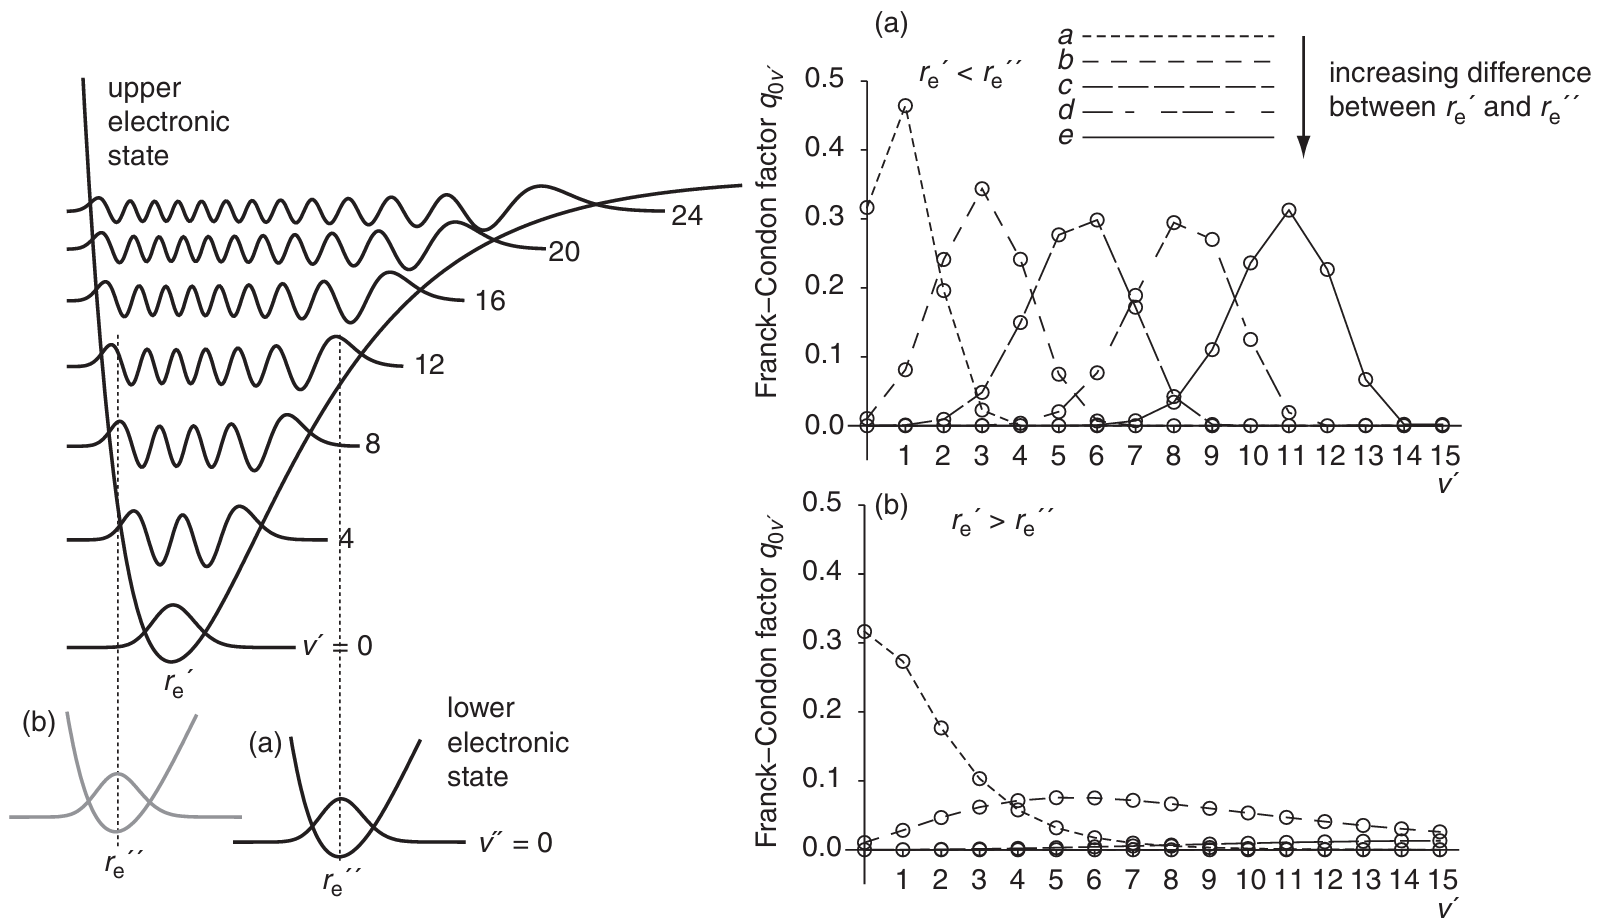
\includegraphics[width=\textwidth]{FC.png}
        \caption{The variation of Franck--Condon factors when the PE curve is anharmonic. Figure adapted from official course note by Prof. Keeler.}
    \end{figure}

    \begin{enumerate}[topsep=0pt]
        \item[(a)] \(r_e'>r_e''\). The maximum in the \(v=0\) wavefunction aligns well with the principal maximum of one of the excited vibrational wavefunctions in the upper electronic state, giving rise to the largest FC factor. Note that on account of the shallowness of the potential, the position of these principal maxima change quite rapidly with the \(v'\) value. The FC factors therefore drop off quite quickly as \(v'\) changes from its optimum value.
        \item[(b)] \(r_e'<r_e''\). The largest FC factors arise when the maximum in the \(v=0\) wavefunction aligns with the subsidiary maxima which occur on the left-hand side of the potential. As the wavefunction is smaller, the maximum FC factors are smaller than in case (a). Note, however, that as the potential is steep the position of these subsidiary maxima changes slowly with \(v'\) so the FC factors are not so sharply peaked.
        \item[(c)] \(r_e'\approx r_e''\). The \(0\rightarrow 0\) transition will be the strongest.
    \end{enumerate}

    The same principles also apply to the emission spectra. The transition will be the strongest when the vibrational ground state wavefunction has its maximum aligned well with the principal maxima of the vibrational wavefunctions for the lower electronic state.\footnote{The official note has a classical explanation for the Franck--Condon factor after this section --- it was stupid so I'm not including it here.}

    \begin{figure}
        \centering
        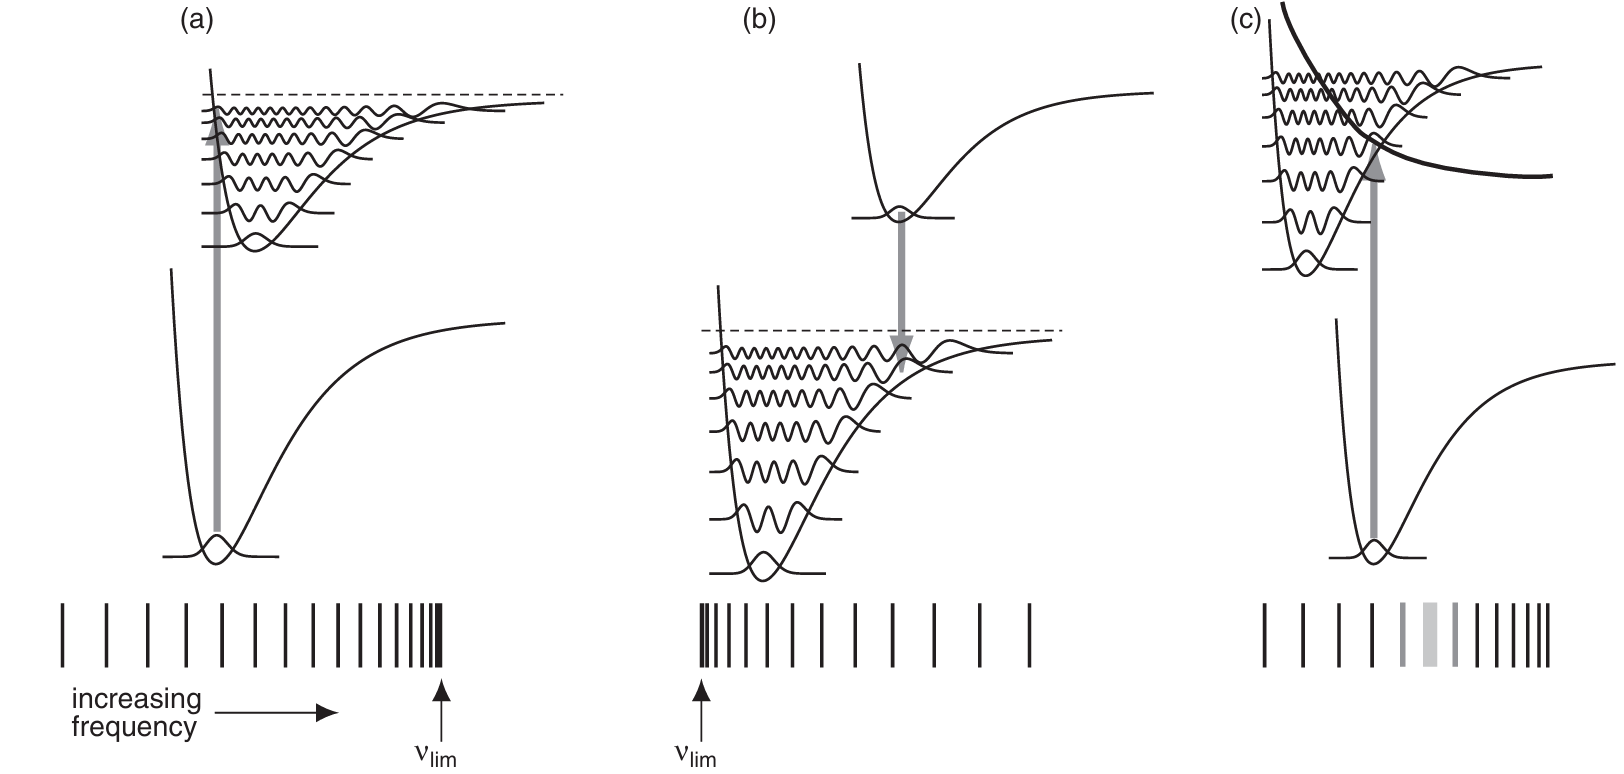
\includegraphics[width=\textwidth]{Dissoc.png}
        \caption{\(\tilde{v}_{\text{lim}}\) observed in (a) absorption, and (b) emission spectra. (c) Pre-dissociation may occur when there are repulsive states. Figure adapted from the official course notes by Prof. Keeler.}
    \end{figure}
    \begin{enumerate}
        \item[(a)] If the Franck--Condon factors are appropriate, we can observe that the lines in a vibrational progression observed in an absorption spectrum will get closer and closer together, reflecting the decreasing spacing of the vibrational energy levels in the upper electronic state. Eventually these levels will converge and, at the dissociation limit of the upper state, become a continuum. The wavenumber at which this occurs is the \(\tilde{\nu}_{\text{lim}}\). This is only likely to be observable if the upper state has a significantly different equilibrium bond length than does the ground state.
        \item[(b)] The dissociation limit of the lower electronic state can be observed in an emission spectrum, once again with the proviso that the FC factors are favourable.
        \item[(c)] It is possible for there to be a \textit{radiationless transition} in which the molecule passes from the bound state over to the repulsive state. Once it does this, the molecule dissociates as the PE simply falls away as the atoms get further apart. This process is called \textit{pre-dissociation}, the name arising from the fact that the molecule dissociates before being promoted to the continuum states of the upper electronic state. The rate of the radiationless transition depends on many factors, including a Franck--Condon-like term involving the overlap of the vibrational wavefunction of the bound state and the (translational) wavefunction of the separated atoms.
        
        Quite often the presence of pre-dissociation leads to a lifetime broadening of the vibrational transitions to states that undergo the radiationless transition. Transitions to higher vibrational levels become sharp once more as they go to states which are not close to the crossing point, and so do not pre-dissociate.
    \end{enumerate}

    \subsubsection{Measurement of Dissociation Energies}
    It is easy to see that
    \begin{align}
        \tilde{D}_0'&=\tilde{\nu}_{\text{lim}}-\tilde{\nu}_{00}\\
        \tilde{D}_0''&=\tilde{\nu}_{\text{lim}}-\Delta\tilde{E}_{\text{atomic}}\,.
    \end{align}
    Unfortunately, it is usually unlikely that the Franck--Condon factors will be sufficiently favourable to observe both \(\tilde{\nu}_{\text{lim}}\) and \(\tilde{\nu}_{00}\). Moreover, it is often rather difficult to identify the atomic states into which a particular molecular state dissociates, so the value of \(\Delta\tilde{E}_{\text{atomic}}\) may not be known.

    A more successful approach is to use what spectroscopic data is available (typically in a progression) and then extrapolate this to find the dissociation energy. The simplest approach is the \textit{Birge--Sponer} extrapolation.

    \begin{figure}[ht!]
        \centering
        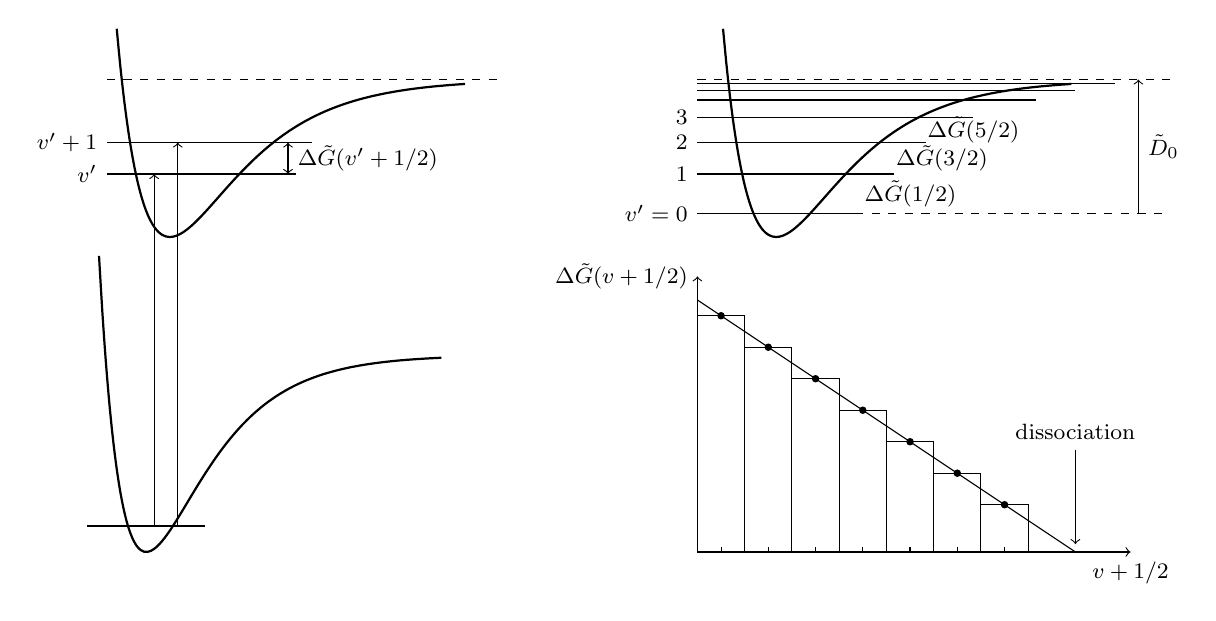
\begin{tikzpicture}
            \draw[thick,domain=-0.4:2.5, smooth, variable=\x,samples=100] plot ({1.5*\x}, {2.5*(1-2.72^(-2*\x))^2});
            \draw (-0.75,0.33)--(0.75,0.33);

            \draw[thick,domain=-0.45:2.5, smooth, variable=\x,samples=100] plot ({1.5*\x+0.3}, {4+2*(1-2.72^(-1.7*\x))^2});
            \draw (-0.5,4.8)node[left]{\footnotesize \(v'\)}--(1.9,4.8);
            \draw (-0.5,5.2)node[left]{\footnotesize \(v'+1\)}--(2.1,5.2);
            \draw[dashed] (-0.5,6)--(4.5,6);

            \draw[->] (0.1,0.33)--(0.1,4.8);
            \draw[->] (0.4,0.33)--(0.4,5.2);
            \draw[<->] (1.8,4.8)--node[right]{\footnotesize\(\Delta\tilde{G}(v'+1/2)\)}(1.8,5.2);

            \draw[thick,domain=-0.45:2.5, smooth, variable=\x,samples=100] plot ({1.5*\x+8}, {4+2*(1-2.72^(-1.7*\x))^2});
            \draw (7,4.3)node[left]{\footnotesize\(v'=0\)}--(9,4.3);
            \draw (7,4.8)node[left]{\footnotesize\(1\)}--(9.5,4.8);
            \draw (7,5.2)node[left]{\footnotesize\(2\)}--(9.9,5.2);
            \draw (7,5.52)node[left]{\footnotesize\(3\)}--(10.5,5.52);
            \draw (7,5.74)--(11.3,5.74);
            \draw (7,5.86)--(11.8,5.86);
            \draw (7,5.95)--(12.3,5.95);
            \draw[dashed] (7,6)--(13,6);
            \node at (9,4.55)[right]{\footnotesize\(\Delta\tilde{G}(1/2)\)};
            \node at (9.4,5)[right]{\footnotesize\(\Delta\tilde{G}(3/2)\)};
            \node at (9.8,5.36)[right]{\footnotesize\(\Delta\tilde{G}(5/2)\)};
            \draw[dashed] (9,4.3)--(13,4.3);
            \draw[->] (12.6,4.3)--node[right]{\footnotesize\(\tilde{D}_0\)}(12.6,6);
            \draw[->] (7,0)--(12.5,0)node[below]{\footnotesize\(v+1/2\)};
            \draw[->] (7,0)--(7,3.5)node[left]{\footnotesize\(\Delta\tilde{G}(v+1/2)\)};
            \foreach \x in {0,...,6}{
                \draw (7.3+0.6*\x,0)--(7.3+0.6*\x,0.06);
                \draw (7+0.6*\x,0) rectangle (7.6+0.6*\x,3-0.4*\x);
                \draw[fill=black] (7.3+0.6*\x,3-0.4*\x) circle (0.04);
            }
            \draw (7,3.2)--(11.8,0);
            \draw[->] (11.8,1.3)node[above]{\footnotesize dissociation}--(11.8,0.1);
        \end{tikzpicture}
    \end{figure}

    Let \(\Delta\tilde{G}(v+\frac{1}{2})\) be the energy separation between the transitions in the same progression with a common lower level and upper vibrational level \(v'\) and \(v'+1\). Then obviously the dissociation energy is
    \begin{equation}
        \tilde{D}_0=\sum\Delta\tilde{G}\left(v+\frac{1}{2}\right)\,.
    \end{equation}

    We can plot a graph of \(\Delta\tilde{G}(v+\frac{1}{2})\) against \(v+\frac{1}{2}\), then the dissociation energy is given by the sum of the area of the rectangles. If there are a sufficiently large number of rectangles, then the sum of their areas is well approximated by the area under the dashed line.

    It may be possible to extrapolate the line to lower or higher values of \(v\) in the case where the data are missing, and so this method is known as the \textit{Birge--Sponer extrapolation}, and the plot is known as the \textit{Birge--Sponer plot}.

    If we want the value of \(\tilde{D}_e\) all we would have to do is extrapolate the line back to correspond to the value \((v+\frac{1}{2})=-\frac{1}{2}\) and take the area from this point. This adds in the energy separation between the bottom of the PE well and the \(v=0\) level. An alternative is to plot \(\Delta\tilde{G}(v+\frac{1}{2})\) against \((v + 1)\) and take the area from zero on the horizontal axis.

    For a Morse potential the Birge--Sponer plot is expected to be a straight line, but in practice it is found that the plot is often curved, especially as \(v\) approaches the dissociation limit when the line tends to fall away. A linear extrapolation is thus like to overestimate the dissociation energy.

    \subsection{Rotational Fine Structure}
    As we noted before, in addition to a change in vibrational energy, the transition between two electronic states may be accompanied by a change in rotational energy. Depending on the term symbols of the electronic states we may have transitions with \(\Delta J=\pm 1\) (\(P\) and \(R\) branches), or with \(\Delta J=0,\pm 1\) (\(P,Q,R\) branches).
    
    The frequencies of the three branches can be easily calculated.
    \begin{align}
        \tilde{\nu}_P&=\tilde{\nu}_{\text{el,vib}}-(\tilde{B}'+\tilde{B}'')J+(\tilde{B}'-\tilde{B}'')J^2\\
        \tilde{\nu}_Q&=\tilde{\nu}_{\text{el,vib}}+J(J+1)(\tilde{B}'-\tilde{B}'')\\
        \tilde{\nu}_R&=\tilde{\nu}_{\text{el,vib}}+2\tilde{B}'+(3\tilde{B}'-\tilde{B}'')J+(\tilde{B}'-\tilde{B}'')J^2\,.
    \end{align}
    Since the \(r_e\) values of the upper and lower electronic states are different, the values of \(\tilde{B}'\) and \(\tilde{B}''\) may differ substantially.

    If \(B'<B''\), the lines in the \(R\) branch get closer together as \(J\) increases, whereas those
    in the \(P\) branch get further apart. The lines in the \(Q\)-branch appear on the low-frequency
    side of \(\tilde{\nu}_{\text{el,vib}}\), which is described by saying that the band is \textit{degraded to the red}.

    On the other hand, if \(B'>B''\), the lines in the \(P\) branch get closer together as \(J\) increases, whereas those in the \(R\) branch get further apart. The lines in the \(Q\) branch appear on the
    high-frequency side of \(\tilde{\nu}_{\text{el,vib}}\), and are said to be \textit{degraded to the blue}.

    \begin{figure}
        \centering
        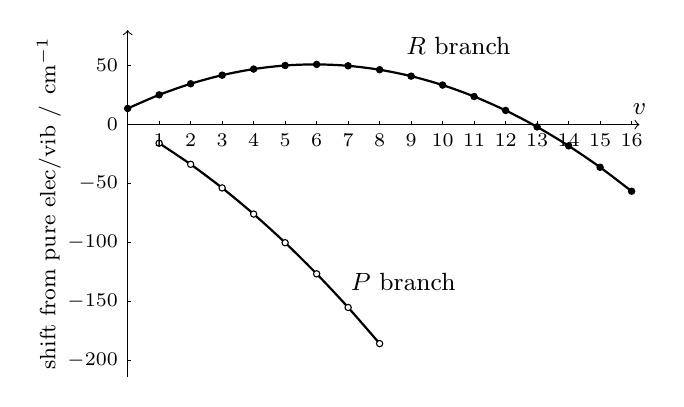
\begin{tikzpicture}
            \draw[->] (0,0)--(6.5,0)node[above]{\small\(v\)};
            \draw[->] (0,-3.2)--(0,1.2);

            \draw[thick,domain=0:16, smooth, variable=\x,samples=17] plot ({0.4*\x}, {(13.64+12.58*\x-1.06*\x*\x)*0.015});
            \foreach \x in {0,...,16}{
                \draw[fill=black] (0.4*\x, 0.2046+0.1887*\x-0.0159*\x*\x) circle (0.04);
            }

            \draw[thick,domain=1:8, smooth, variable=\x,samples=8] plot ({0.4*\x}, {(-14.7*\x-1.06*\x*\x)*0.015});
            \foreach \x in {1,...,8}{
                \draw[fill=white] (0.4*\x, -0.2205*\x-0.0159*\x*\x) circle (0.04);
            }

            \foreach \x in {1,...,16}{
                \draw (0.4*\x,0.05)--(0.4*\x,0)node[below]{\scriptsize\(\x\)};
            }
            \foreach \y in {-200,-150,-100,-50,0,50}{
                \draw (0.04,0.015*\y)--(0,0.015*\y)node[left]{\scriptsize\(\y\)};
            }
            \node[rotate=90] at (-1,-1) {\footnotesize shift from pure elec/vib / \(\!\unit{cm}^{-1}\)};
            \node at (4.2,1) {\small \(R\) branch};
            \node at (3.5,-2) {\small \(P\) branch};
        \end{tikzpicture}
        \caption{The \(P\) and \(R\) branches for \(\tilde{B}'=6.82\unit{cm}^{-1}\), \(\tilde{B}''=7.88\unit{cm}^{-1}\). The value corresponds to the \(A\ ^1\Sigma^+\leftarrow X \ ^1\Sigma^+\) transition in \(\mathrm{CuH}\).}
    \end{figure}

    The figure above shows when \(\tilde{B}'<\tilde{B}''\). The lines in the \(R\) branch at first increase in frequency, but their spacings are steadily decreasing. Eventually the (negative) quadratic term starts to dominate over the linear term, resulting in the lines reaching a maximum frequency and then moving back to lower frequencies. The highest frequency reached by the lines in the \(R\) branch is called a \textit{band head}.

    A band head is often visible in the spectrum as an intense feature since several lines are bunched in this region. In addition, the feature has a sharp edge as all the lines are at lower frequencies than this band head.

    \begin{figure}
        \centering
        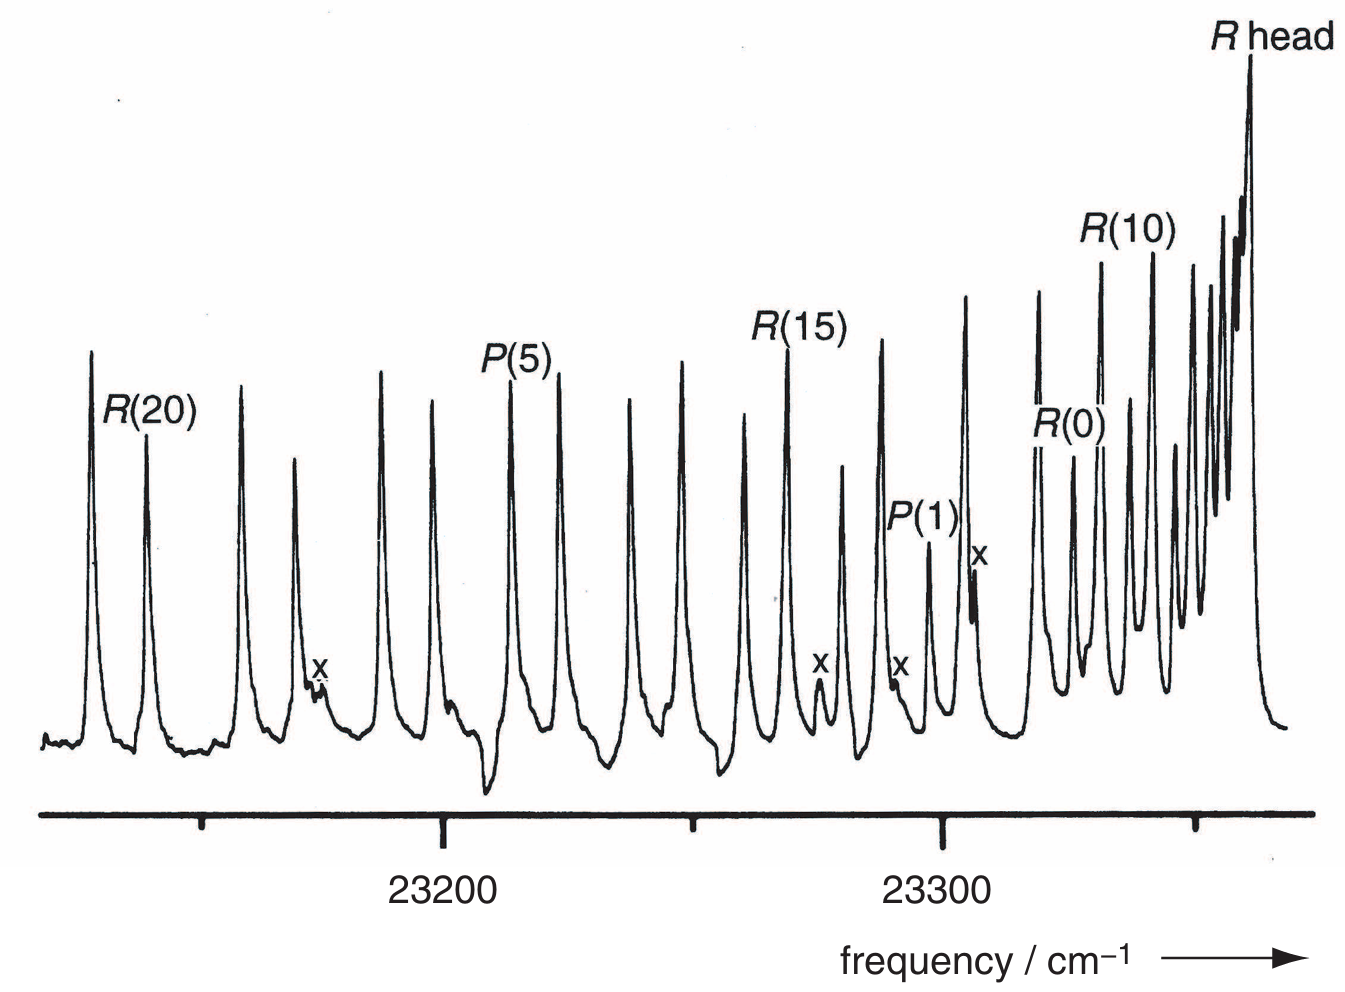
\includegraphics[width=0.6\textwidth]{band_head.png}
        \caption{The spectrum for \(\mathrm{CuH}\) in which the band head structure in the \(R\) branch is clearly seen. Figure adapted from Banwell.}
    \end{figure}

    In this case the \(R\) branch is said to be \textit{degraded to the red}, as it turns around and heads off to lower frequencies. In contrast, the lines in the \(P\) branch simply head off to lower frequencies in a consistent manner.

    If \(B'>B''\) then the band head appears in the \(P\) branch, and this would be \textit{degraded to the blue}. Which branch the band head appears in is thus diagnostic of the relative sizes of
    \(B'\) and \(B''\).

    We can locate the position of the band head by differentiating the expression for the lines in the \(P\) or \(R\) branch (as appropriate) with respect to \(J\) and then finding the turning point. The calculation is trivial and we find
    \begin{align}
        R\text{ branch: }J_{\text{head}}&=\frac{\tilde{B}''-3\tilde{B}'}{2(\tilde{B}'-\tilde{B}'')}\\
        P\text{ branch: }J_{\text{head}}&=\frac{\tilde{B}'+\tilde{B}''}{2(\tilde{B}'-\tilde{B}'')}\,.
    \end{align}
    Evaluating this expression with the data given above for \(\mathrm{CuH}\) gives \(J_{\text{head}}=5.93\), so the band head occurs at either \(J=5\) or \(6\). By comparing the values, we find the band head is the line \(R(6)\), which fits in with the graph.

    \newpage

    \section{Fluorescence and Phosphorescence}
    The electronic spectra of molecules larger than diatomics rapidly become very complex as a result of the large number of electronic states and the vibrational fine structure arising from many normal modes. Spectra typically show broad absorption maxima which arise from the overlap of many bands. If we move from the gas phase to solution the situation is made even worse as a result of interactions with the solvent giving further broadening.

    Despite the lack of resolved fine structure there is considerable interest in the electronic spectra of larger molecules as a result of the phenomena of \textit{fluorescence} and \textit{phosphorescence} which these molecules often show.
    
    When a molecule is excited to a higher electronic state by the absorption of light of a particular wavelength it is often found that the molecule starts to emit light at a somewhat longer wavelength. Sometimes it is found that this emission of light stops very soon after the excitation is removed: the emission is then termed \textit{fluorescence}. Sometimes it is found that the emission continues for a significant time after the excitation is removed: this is termed \textit{phosphorescence}.

    \subsection{Fluorescence}
    \begin{figure}[ht!]
        \centering
        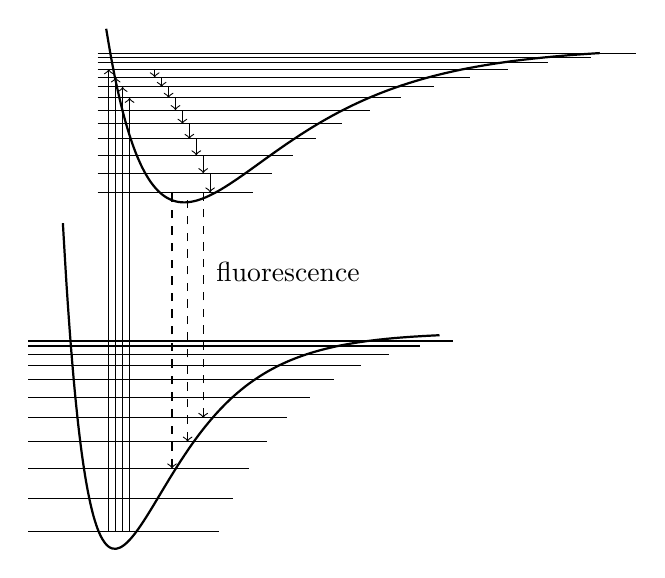
\begin{tikzpicture}[scale=1.1]
            \draw[thick,domain=-0.4:2.5, smooth, variable=\x,samples=100] plot ({1.5*\x}, {2.5*(1-2.72^(-2*\x))^2});
            \foreach \x in {0,...,10}{
                \draw (-1,0.2+0.4*\x-0.018*\x*\x)--(1.2+0.15*\x+0.012*\x*\x,0.2+0.4*\x-0.018*\x*\x);
            }

            \draw[thick,domain=-0.6:3.2, smooth, variable=\x,samples=100] plot ({1.5*\x+0.8}, {4+1.8*(1-2.72^(-1.2*\x))^2});
            \foreach \x in {0,...,12}{
                \draw (-0.2,4.115+0.23*\x-0.008*\x*\x)--(1.6+0.2*\x+0.014*\x*\x,4.115+0.23*\x-0.008*\x*\x);
            }
            \foreach \x in {6,7,8,9}{
                \draw[->] (0.65-0.08*\x,0.2)--(0.65-0.08*\x,4.115+0.23*\x-0.008*\x*\x);
            }
            \foreach \x in {0,...,8}{
                \draw[<-] (1.1-0.08*\x,4.115+0.23*\x-0.008*\x*\x)--(1.1-0.08*\x,4.337+0.214*\x-0.008*\x*\x);
            }
            \foreach \x in {2,3,4}{
                \draw[<-,dashed] (0.3+0.18*\x,0.2+0.4*\x-0.018*\x*\x)--(0.3+0.18*\x,4.115);
            }
            \node at (2,3.2) {fluorescence};
        \end{tikzpicture}
    \end{figure}
    The diagram above can be used to explain the basic features of fluorescence. It shows the ground electronic state and an excited electronic state which, as is often the case, is less tightly bound than the ground state. Typically the ground vibrational state of the ground electronic state will be by far the most populated level. As a result of the displacement of the potential energy curve of the excited state, the Franck--Condon principle indicates that the strongest transitions in absorption will be to excited vibrational states. If the molecule is in solution it undergoes frequent collisions in which this excess vibrational energy will be lost and so the molecule quickly ends up in the ground vibrational state of the excited electronic state. This process is called \textit{vibrational relaxation}.

    Vibrational relaxation is relatively efficient as the amount of energy that needs to be lost in each step down the ladder of vibrational levels is, for large molecules in particular, small compared to thermal energies; in addition, in solution collisions are frequent. In contrast, it is more difficult for the molecule to lose the much larger amount of energy which would take it back to the ground electronic state.

    Spontaneous emission then occurs from the ground vibrational state of the excited electronic state back down to the ground electronic state; the Franck--Condon principle indicates that the strongest transitions will be to excited vibrational states. This emission is termed fluorescence.

    This mechanism provides an explanation of the key features of fluorescence:
    \begin{enumerate}[topsep=0pt,label=(\roman*)]
        \item Fluorescence occurs at a longer wavelength than the absorption as a result of the loss of energy due to vibrational relaxation.
        \item The absorption spectrum shows vibrational fine structure characteristic of the excited electronic state, whereas the fluorescence spectrum shows vibrational structure characteristic of the ground electronic state --- this is the result of the Franck--Condon factors and that both spectra originate from ground vibrational states.
        \item The emission stops once the exciting radiation is removed: without the excitation, there is no process to populate the excited state from which emission occurs.
    \end{enumerate}

    \subsubsection{Fluorescence Spectra}
    The schematic arrangement of a fluorescence spectrometer is shown below.
    \begin{figure}[ht!]
        \centering
        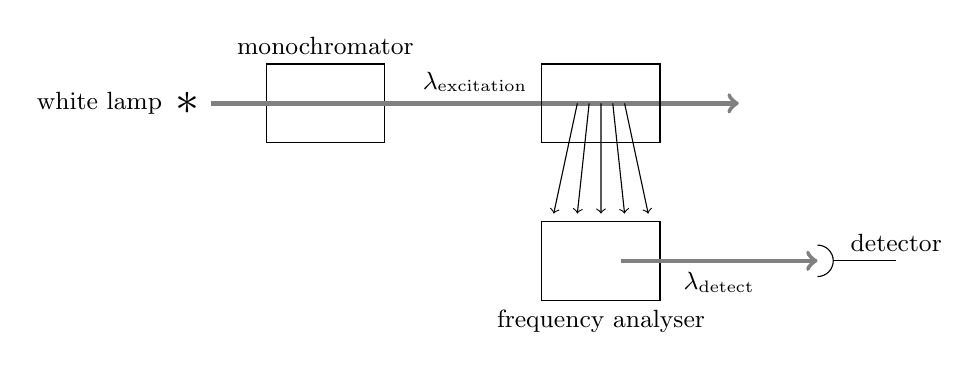
\begin{tikzpicture}
            \draw (0,0) rectangle (1.5,1);
            \node at (0.75,1) [above]{\small monochromator};
            \node at (-1,0.5) {\LARGE \(*\)};
            \node at (-1.2,0.5) [left] {\small white lamp};
            \draw[ultra thick,gray,->] (-0.7,0.5)--node[above,black]{\small \(\lambda_{\text{excitation}}\)}(6,0.5);
            \draw (3.5,0) rectangle (5,1);
            \foreach \x in {0,...,4}{
                \draw[->] (3.95+0.15*\x,0.5)--(3.65+0.3*\x,-0.9);
            }
            \draw (3.5,-2) rectangle (5,-1);
            \draw[ultra thick, gray,->] (4.5,-1.5)--node[below,black]{\small\(\lambda_{\text{detect}}\)}(7,-1.5);
            \node at (4.25,-2) [below] {\small frequency analyser};
            \draw (7,-1.3) arc (90:-90:0.2);
            \draw (7.2,-1.5)--(8,-1.5)node[above]{\small detector};
        \end{tikzpicture}
    \end{figure}

    The \textit{fluorescence spectrum} is usually recorded by fixing the wavelength of the exciting radiation \(\lambda_{\text{excitation}}\) (at a position where there is significant absorption) and then measuring the emission at different wavelengths \(\lambda_{\text{detect}}\). The experimental arrangement involves detecting the emitted light at right angles to the beam of exciting radiation so as to avoid swamping the detector with very intense radiation normally used for excitation. According to the above model, the frequencies of the features in the fluorescence spectrum are independent of the frequency of the exciting radiation, but we may expect the intensity to vary as the frequency of the exciting radiation varies.

    It is also possible to record the excitation spectrum in which we detect at a fixed frequency (where fluorescence is expected) and then scan the frequency of the exciting radiation. According to the model above, the excitation spectrum should have the same form as the absorption spectrum.

    \begin{figure}
        \centering
        \begin{tikzpicture}
            \node at (0,0){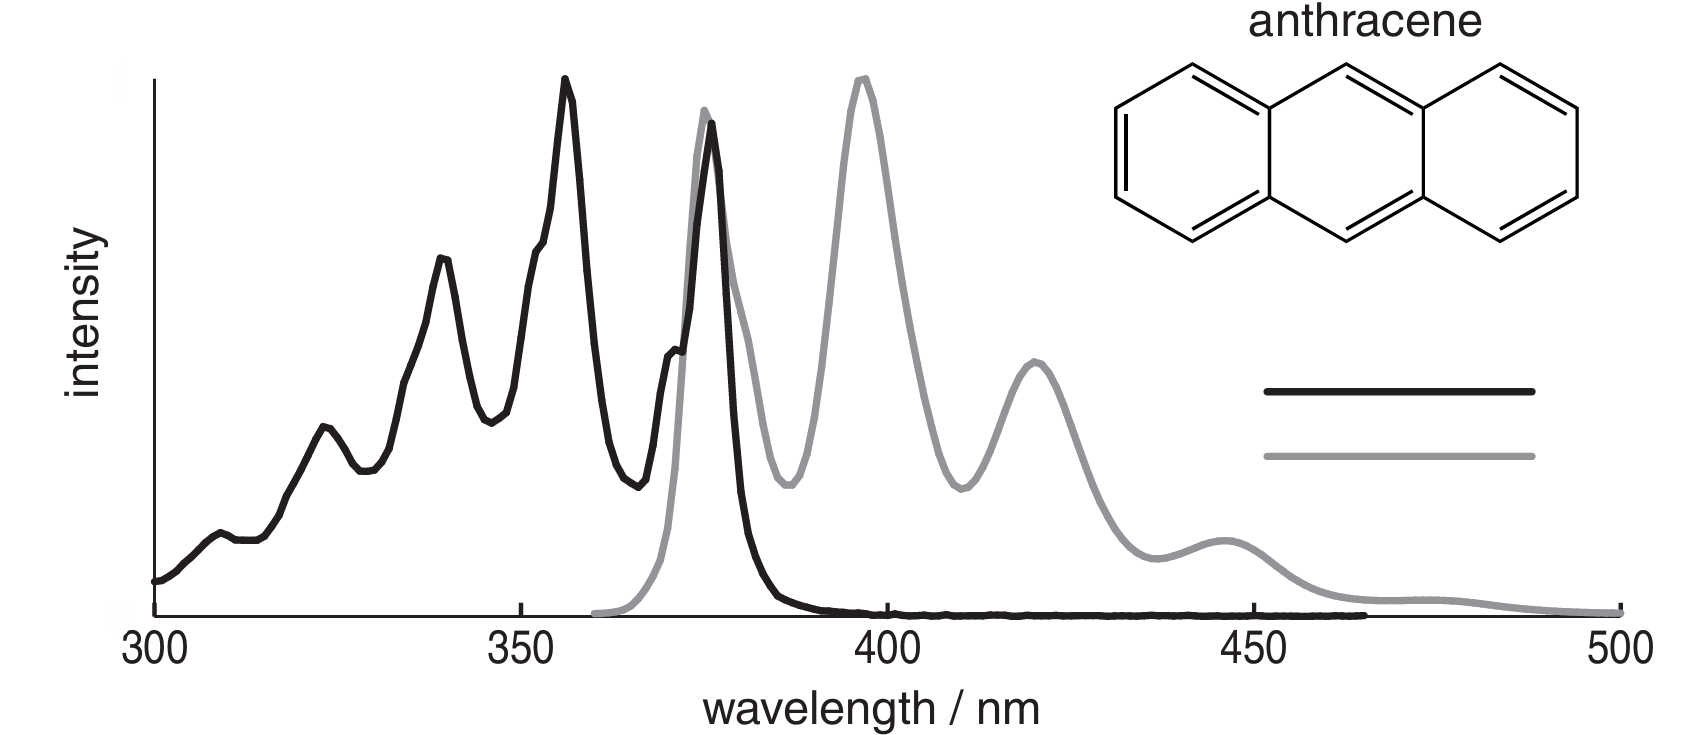
\includegraphics[width=0.7\textwidth]{anth_fluo.png}};
            \node at (4.4,-0.15)[right]{\small absorption};
            \node at (4.4,-0.55)[right]{\small fluorescence};
        \end{tikzpicture}
        \caption{The fluorescence spectrum of anthracene using cyclohexane as solvent. This figure (and all the other fluorescence spectra below) is adapted from a database maintained by the University of Arizona, available at http://www.spectra.arizona.edu.}
    \end{figure}

    Shown below are the absorption and fluorescence spectra of anthracene (in cyclohexane as solvent). As expected, we see the fluorescence spectrum centred at a lower frequency (longer wavelength) than the absorption spectrum. In this case the two spectra overlap to a significant extent, and the fine structure appears to be quite similar; the overlapping peak is likely to be due to the \(0\rightarrow 0\) transition. From this we may infer that the ground and excited electronic states do not differ too much in equilibrium geometry. In such a situation the absorption and fluorescence spectra are approximate mirror images of one another.

    \begin{figure}
        \centering
        \begin{tikzpicture}
            \node at (0,0){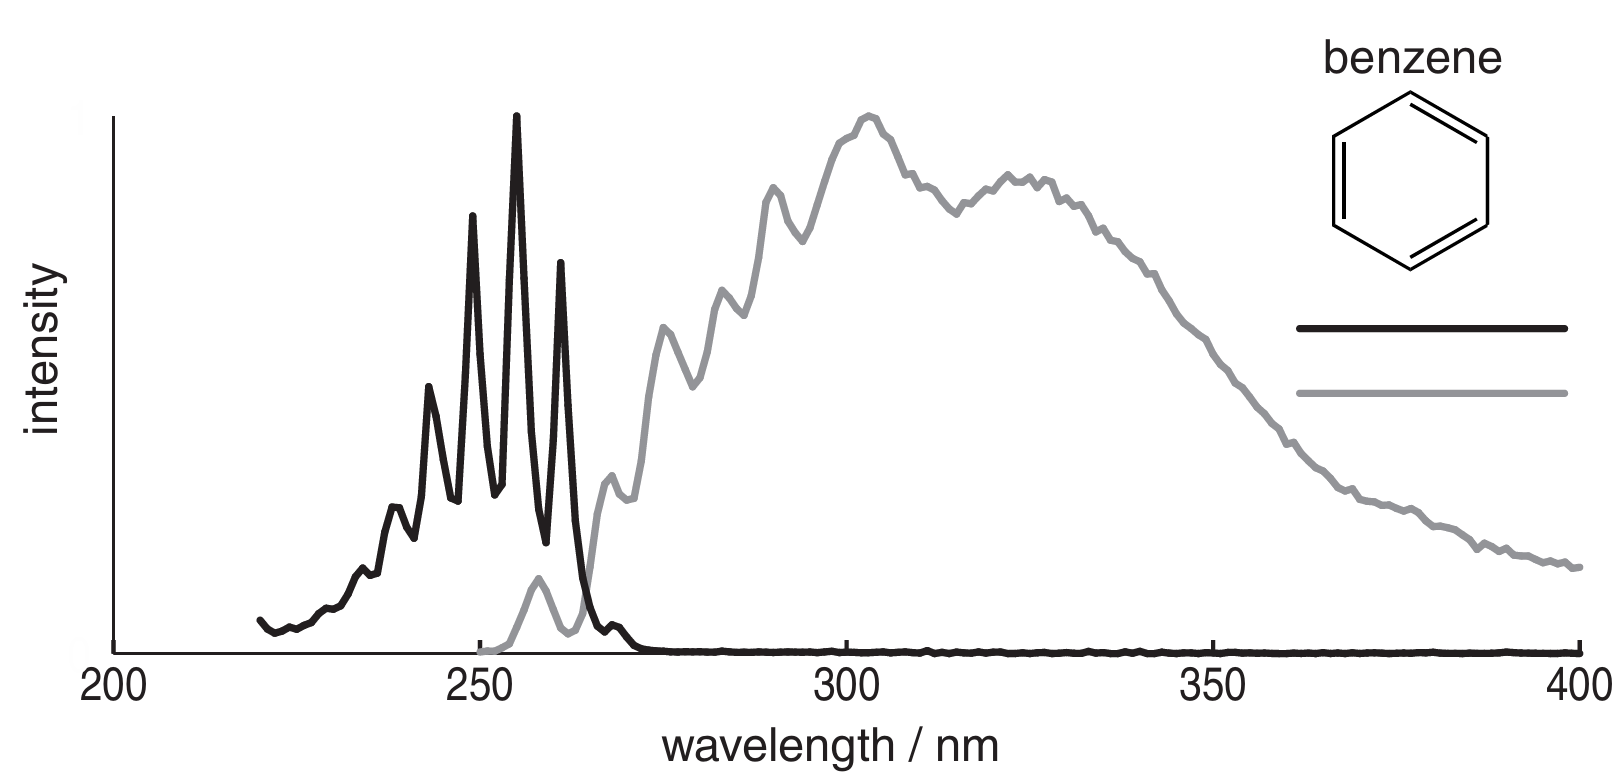
\includegraphics[width=0.7\textwidth]{ben_fluo.png}};
            \node at (5,0.4)[right]{\small absorption};
            \node at (5,0)[right]{\small fluorescence};
        \end{tikzpicture}
        \caption{The fluorescence spectrum of benzene using cyclohexane as solvent.}
    \end{figure}

    The spectra for benzene are quite different. Here we see a much larger shift between the principal maxima in the absorption and fluorescence spectra, as well as substantially different vibrational fine structure. From this we can infer that the ground and excited electronic states differ significantly in their equilibrium geometry.

    \subsubsection{Jablonski Diagram}
    It is common to discuss fluorescence and related phenomena using a schematic representation of the electronic and vibrational energy levels called a \textit{Jablonski diagram}.
    \begin{figure}[ht!]
        \centering
        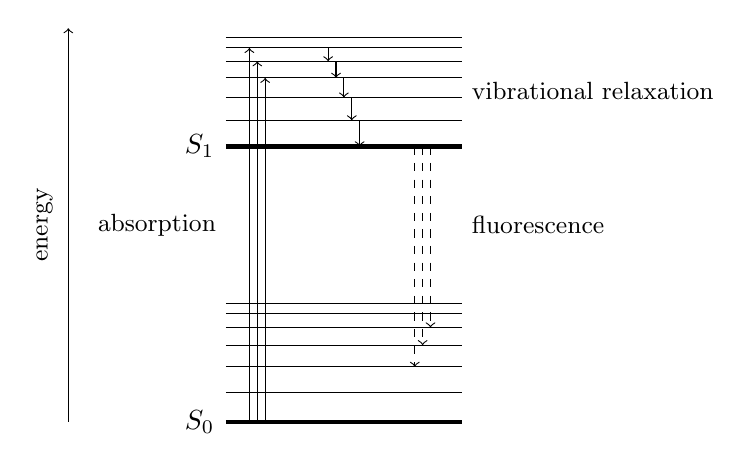
\begin{tikzpicture}
            \draw[->] (-2,0)--(-2,5);
            \node[rotate=90] at (-2.3,2.5) {\small energy};
            \draw[ultra thick] (0,0)node[left]{\(S_0\)}--(3,0);
            \draw[ultra thick] (0,3.5)node[left]{\(S_1\)}--(3,3.5);
            \foreach \x in {1,...,6}{
                \draw (0,0.4*\x-0.025*\x*\x)--(3,0.4*\x-0.025*\x*\x);
                \draw (0,3.5+0.35*\x-0.02*\x*\x)--(3,3.5+0.35*\x-0.02*\x*\x);
            }
            \foreach \x in {3,4,5}{
                \draw[->] (0.8-0.1*\x,0)--(0.8-0.1*\x,3.5+0.35*\x-0.02*\x*\x);
            }
            \foreach \x in {0,...,4}{
                \draw[<-] (1.7-0.1*\x,3.5+0.35*\x-0.02*\x*\x)--(1.7-0.1*\x,3.83+0.31*\x-0.02*\x*\x);
            }
            \foreach \x in {2,3,4}{
                \draw[->,dashed] (2.2+0.1*\x,3.5)--(2.2+0.1*\x,0.4*\x-0.025*\x*\x);
            }
            \node at (0,2.5)[left]{\small absorption};
            \node at (3,4.2)[right]{\small vibrational relaxation};
            \node at (3,2.5)[right]{\small fluorescence};
        \end{tikzpicture}
    \end{figure}

    The thick lines represent the energies of the (pure) electronic states, and built on these is a set of vibrational levels, shown schematically. In most molecules all of the spins are paired up in the ground electronic state, thus the total spin \(S\) is zero, and hence the state is a spin singlet. The ground state in the Jablonski diagram is therefore labelled \(S_0\).

    Since the selection rule for \(S\) is \(\Delta S=0\), the excited state to which there is strong absorption is also likely to be a singlet, and here it is labelled \(S_1\); further higher energy singlet states are labelled \(S_2\) etc.
    
    In terms of the Jablonski diagram, fluorescence would be described as absorption from the ground vibrational state of \(S_0\) to various excited vibrational states of \(S_1\), followed by vibrational relaxation down to the ground vibrational state of \(S_1\). Fluorescence arises from transitions from the ground vibrational state of \(S_1\) down to various excited vibrational states of \(S_0\).

    \subsubsection{Solvent Effect}
    The initial transition caused by absorption of the exciting photons is very fast so that when the molecule is promoted to the \(S_1\) state its geometry is, to start with, the same as it had in the ground state; in the language of the Franck--Condon principle, such transitions are said to be vertical. It is likely that the equilibrium geometry of the \(S_1\) state is different to that of the \(S_0\) state, so \(S_1\) will be produced in an excited vibrational state (as predicted by the Franck--Condon principle). Subsequent vibrational relaxation will allow \(S_1\) to drop down to its ground vibrational state and achieve its equilibrium geometry.

    If the molecule is in solution there are additional effects due to changes in solvation. When it is produced the \(S_1\) state will be surrounded by solvent molecules which are arranged for the optimum solvation of the \(S_0\) state. Not only is it likely that the equilibrium geometry of \(S_1\) is different from \(S_0\), but it is also likely that the electron distribution is different; as a result the solvent needs to adapt itself to both the new geometry and the new electron distribution. The overall effect of this is that the energy of the excited state falls slightly as the solvent adjusts itself to the new geometry.

    When it comes to the fluorescent transition similar considerations apply. The vertical transition initially produces \(S_0\) with the equilibrium geometry of \(S_1\), and the solvation appropriate for \(S_1\). As the molecule shifts to the equilibrium geometry of \(S_0\), and the solvent accommodates to this change, the energy will fall. These points are illustrated schematically in the diagram.

    \begin{figure}
        \centering
        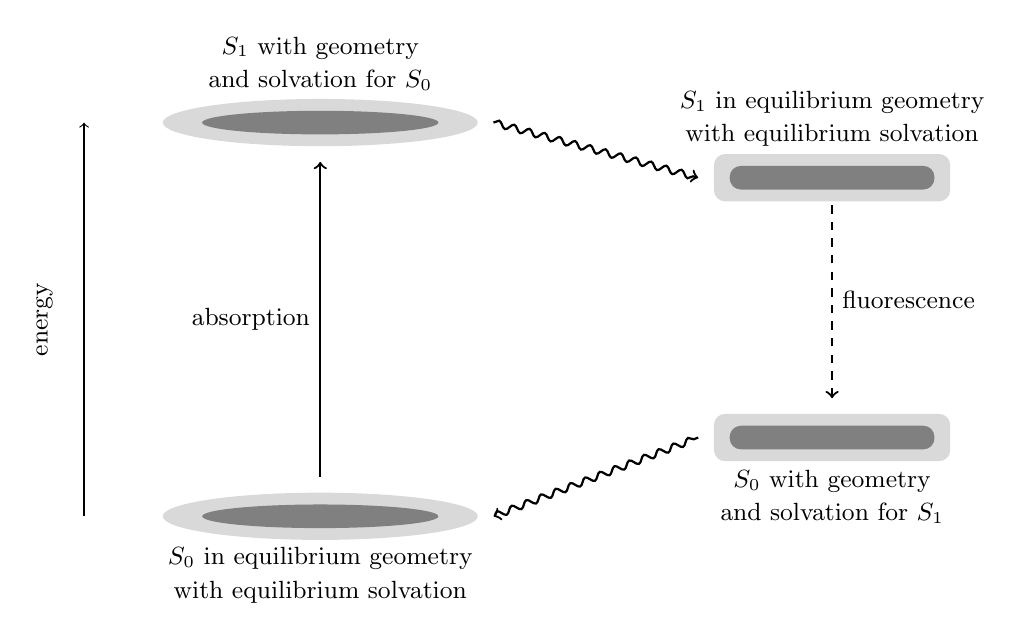
\begin{tikzpicture}
            \draw[->] (-3,0)--(-3,5);
            \node[rotate=90] at (-3.5,2.5){\small energy};
            \fill[gray!30] (0,0) ellipse (2cm and 0.3cm);
            \fill[gray] (0,0) ellipse (1.5cm and 0.15cm);
            \fill[gray!30] (0,5) ellipse (2cm and 0.3cm);
            \fill[gray] (0,5) ellipse (1.5cm and 0.15cm);
            \draw[thick,->] (0,0.5)--node[left]{\small absorption}(0,4.5);
            \node[align=center] at (0,-0.75) {\small \(S_0\) in equilibrium geometry \\ \small with equilibrium solvation};
            \node[align=center] at (0,5.75) {\small \(S_1\) with geometry \\ \small and solvation for \(S_0\)};
            \fill[gray!30,rounded corners] (5,4) rectangle (8,4.6);
            \fill[gray,rounded corners] (5.2,4.15) rectangle (7.8,4.45);
            \fill[gray!30,rounded corners] (5,0.7) rectangle (8,1.3);
            \fill[gray,rounded corners] (5.2,0.85) rectangle (7.8,1.15);
            \node[align=center] at (6.5,0.25) {\small \(S_0\) with geometry \\ \small and solvation for \(S_1\)};
            \node[align=center] at (6.5,5.05) {\small \(S_1\) in equilibrium geometry \\ \small with equilibrium solvation};
            \draw[thick,dashed,<-] (6.5,1.5)--node[right]{\small fluorescence}(6.5,4);
            \draw[decoration = {snake,amplitude=1.2pt,segment length=2mm},decorate,->,thick] (2.2,5)--(4.8,4.3);
            \draw[decoration = {snake,amplitude=1.2pt,segment length=2mm},decorate,<-,thick] (2.2,0)--(4.8,1);
        \end{tikzpicture}
    \end{figure}

    The net result of these solvent effects is that the fluorescence is shifted to longer wavelengths. This is most clearly seen in cases where the \(v''=0\leftrightarrow v'=0\) transition is visible in both the absorption and fluorescence spectrum. Simple considerations would indicate that this transition should have the same wavelength in both spectra, but in fact it is seen that the wavelength is slightly longer in the fluorescence spectrum --- an effect which is accounted for by the solvent effects discussed here. The effect is greater for more polar solvents.

    This medium-induced shift in the wavelength of the fluorescence has been exploited extensively in the study of proteins. When excited at \(290\unit{nm}\), the (naturally occurring) amino acid tryptophan shows a fluorescence maximum at around \(356\unit{nm}\) in aqueous solution. Changing the solvent to dioxane, which is less polar, moves the fluorescence maximum to around \(320\unit{nm}\).

    Hence a tryptophan buried inside the protein in a hydrophobic environment we might expect a fluorescence maximum at a shorter wavelength than would be the case if the tryptophan was on the surface of the protein and exposed to polar solvent. This shift in the fluorescence maximum can also be used to study the unfolding of a protein. Suppose that the protein has a tryptophan which, in the folded form of the protein, is in a hydrophobic environment. When the protein unfolds, the tryptophan is exposed to the polar solvent and so the fluorescence maximum moves to a longer wavelength. By monitoring the onset of fluorescence at this longer wavelength we can therefore assess the extent to which the protein is unfolded.

    \subsection{Phosphorescence}
    The characteristic feature of phosphorescence is that the emission continues from some time after the exciting radiation has been removed. The accepted explanation for this is that the transition involved in the phosphorescent emission is from an excited triplet state down to the singlet ground state. Such a transition is forbidden by the spin selection rule so the spontaneous emission rate is much less than for a singlet-singlet transition. The excited triplet state can therefore build up a population which only decays away slowly, hence accounting for the persistence of the phosphorescent emission. How the triplet state is populated in the first place is conveniently described using a Jablonski diagram.

    \begin{figure}[ht!]
        \centering
        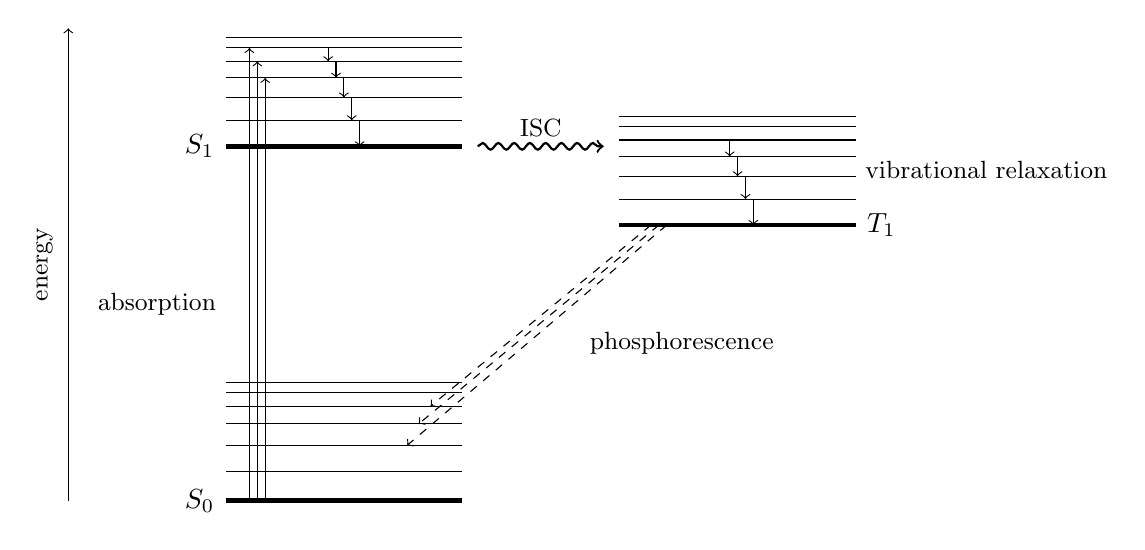
\begin{tikzpicture}
            \draw[->] (-2,0)--(-2,6);
            \node[rotate=90] at (-2.3,3) {\small energy};
            \draw[ultra thick] (0,0)node[left]{\(S_0\)}--(3,0);
            \draw[ultra thick] (0,4.5)node[left]{\(S_1\)}--(3,4.5);
            \draw[ultra thick] (5,3.5)--(8,3.5)node[right]{\(T_1\)};
            \draw[decoration = {snake,amplitude=1.2pt,segment length=2mm},decorate,->,thick] (3.2,4.5)--node[above]{\small ISC}(4.8,4.5);
            \foreach \x in {1,...,6}{
                \draw (0,0.4*\x-0.025*\x*\x)--(3,0.4*\x-0.025*\x*\x);
                \draw (0,4.5+0.35*\x-0.02*\x*\x)--(3,4.5+0.35*\x-0.02*\x*\x);
                \draw (5,3.5+0.35*\x-0.02*\x*\x)--(8,3.5+0.35*\x-0.02*\x*\x);
            }
            \foreach \x in {3,4,5}{
                \draw[->] (0.8-0.1*\x,0)--(0.8-0.1*\x,4.5+0.35*\x-0.02*\x*\x);
            }
            \foreach \x in {0,...,4}{
                \draw[<-] (1.7-0.1*\x,4.5+0.35*\x-0.02*\x*\x)--(1.7-0.1*\x,4.83+0.31*\x-0.02*\x*\x);
            }
            \foreach \x in {0,...,3}{
                \draw[<-] (6.7-0.1*\x,3.5+0.35*\x-0.02*\x*\x)--(6.7-0.1*\x,3.83+0.31*\x-0.02*\x*\x);
            }
            \foreach \x in {2,3,4}{
                \draw[->,dashed] (5.8-0.1*\x,3.5)--(2+0.15*\x,0.4*\x-0.025*\x*\x);
            }
            \node at (0,2.5)[left]{\small absorption};
            \node at (8,4.2)[right]{\small vibrational relaxation};
            \node at (4.5,2)[right]{\small phosphorescence};
        \end{tikzpicture}
    \end{figure}

    As before, absorption followed by vibrational relaxation results in population of the ground vibrational state of \(S_1\). Under the right circumstances it is then possible for there to be a radiationless transition taking the molecule from \(S_1\) to \(T_1\): this is called \textit{intersystem crossing}, ISC. This process populates excited vibrational levels of \(T_1\), but as before we expect collisions to result in rapid vibrational relaxation resulting in population of the ground vibrational state. The phosphorescent emission occurs from the ground vibrational state of \(T_1\) to various vibrational states of \(S_0\). This triplet-singlet transition is forbidden by the spin selection rule so the rate of emission is much slower than for the allowed singlet-singlet transition. It is therefore possible for ISC to build up a population of the \(T_1\) state which persists even after the exciting radiation has been removed.

    We can think of intersystem crossing as a process in which the wavefunction for \(S_1\) evolves over time into the wavefunction for \(T_1\). Such a process is formally forbidden in the same way that a singlet-triplet spectroscopic transition is forbidden by the \(\Delta S=0\) selection rule, but in the presence of spin-orbit coupling the selection rule starts to break down and both ISC and singlet-triplet spectroscopic transitions become possible to some extent. Recall that spin-orbit coupling is the interaction between the magnetic moments due to electron spin and the orbital motion of the electrons. Such interactions increase markedly as the atomic number of the atom increases, so the presence of heavy atoms, such as \(\mathrm{Br}\) or \(\mathrm{I}\), will lead to a significant rate of ISC.

    Intersystem crossing is only efficient between states with the same energy. It is unlikely that the pure electronic states \(S_1\) and \(T_1\) will have the same energy, but as these states also have many vibrational levels associated with them there is a good chance of finding a pair of vibrational levels in the two electronic states whose energies match --- this is all the more likely for larger molecules which have many, densely-packed vibrational levels.

    \subsubsection*{Timescales}
    The time scales for the various processes involved in fluorescence and phosphorescence vary considerably with both the molecule involved and the medium. Some representative ranges are
    \begin{itemize}[topsep=0pt]
        \item vibrational relaxation: \(10^{-11}\sim 10^{-9}\unit{s}\).
        \item fluorescence: \(10^{-8}\sim 10^{-4}\unit{s}\).
        \item ISC: \(10^{-12}\sim 10^{-4}\unit{s}\).
        \item phosphorescence: \(10^{-4}\sim 10^{2}\unit{s}\)
    \end{itemize}

    \subsubsection*{Internal Conversion}
    \textit{Internal conversion} (IC) is a similar process to ISC except that it involves two electronic states of the same multiplicity i.e. two singlets. Like ISC, IC will only be efficient between levels with the same energy, so IC between \(S_1\) and \(S_0\) would have to involve very highly excited vibrational levels of \(S_0\). After IC, vibrational relaxation would quickly take us down to the lower vibrational levels of \(S_0\). The net result of IC is to remove electronically excited states.

    \subsection{Kinetics of Excited States}
    The various process involving the generation and interconversion of these excited electronic states can be analysed using a kinetic scheme, just as we would for a series of interconnected chemical reactions. This analysis leads to predictions which can be tested experimentally, and to methods for measuring the rate constants of some of the individual processes.

    \subsubsection{Fluorescence Lifetime and Quantum Yield}
    For each of the processes we have discussed so far we can write a rate in terms of a relevant rate constant and concentration. These are summarized in the table below.

    \renewcommand{\arraystretch}{1.2}
    \begin{table}[ht!]
        \centering
        \begin{tabular}{lll}
            \toprule
            process & equation & rate \\ \midrule
            absorption & \(S_0+h\nu_{\text{excitation}}\to S_1\) & \(I_{\text{abs}}\) \\
            fluorescence & \(S_1\to S_0+h\nu_{\text{fluor}}\) & \(k\FF[S_1]\) \\
            IC & \(S_1\to S_0\) & \(k\IC[S_1]\) \\
            ISC & \(S_1\to T_1\) & \(k\ISC[S_1]\) \\ \bottomrule
        \end{tabular}
    \end{table}

    \subsubsection*{Measurement of the Fluorescence Lifetime}
    The simplest case to analyse is just after the exciting irradiation has been switched off. Now, no more \(S_1\) states are being generated but there are three processes which contribute to the decay of \(S_1\). Since all of these processes are first-order in \([S_1]\), the rate constant for the overall decay of \(S_1\) is simply the sum of the three individual rate constants. It therefore follows that \([S_1]\) decays exponentially according to
    \begin{equation}
        [S_1](t)=[S_1](0)\exp\left[-(k\FF+k\IC+k\ISC)t\right]\,.
    \end{equation}
    We can define the fluorescence lifetime as
    \begin{equation}
        \tau_0=\frac{1}{k\FF+k\IC+k\ISC}\,.
    \end{equation}
    It is possible to measure this lifetime by measuring the decay in the intensity of fluorescence after the excitation has been switched off. Typically this might be done by exciting the molecules using a brief pulse from a laser and then following the decay after the pulse.

    \subsubsection*{Fluorescence Quantum Yield}
    Each photon that is absorbed creates a molecule in the \(S_1\) state, but there are several possible fates of this excited state, only one of which gives rise to the emission of a (fluorescent) photon. We can define the \textit{quantum yield of fluorescence}, \(\phi\FF\), as the ratio of the number of fluorescent photons to the number of photons absorbed
    \begin{equation}
        \phi\FF=\frac{\text{number of fluorescent photons}}{\text{number of photons absorbed}}\,.
    \end{equation}
    If each photon absorbed gives rise to the emission of a fluorescent photon, the quantum yield is \(1\); if other processes destroy the \(S_1\) states, the quantum yield will be less than \(1\). The quantum yield can equally well be defined in terms of rates
    \begin{equation}
        \phi\FF=\frac{\text{rate of fluorescence}}{\text{rate of absorption}}\,.
    \end{equation}
    \subsubsection*{Steady-State Measurements}
    Imagine an experiment in which the exciting radiation is applied continuously to the sample and the intensity of the fluorescence is measured.  This is called a \textit{steady-state experiment}, in contrast to the time-resolved experiment described above for the measurement of the fluorescence lifetime. We can derive an expression for \(\phi\FF\) by invoking the steady-state approximation for \([S_1]\); this will be valid provided the intensity of the exciting radiation is not too great. Assuming the steady state we find:
    \begin{equation}
        [S_1]_{\text{SS}}=\frac{I_{\text{abs}}}{k\FF+k\IC+k\ISC}\,.
    \end{equation}
    Note that the rate of absorption of photons has been written as \(I_{\text{abs}}\), which subsumes the overall concentration of the absorbing molecules and the flux of exciting photons. Using this to find an expression for \([S_1]_{\text{SS}}\) we can then proceed to use this to find \(\phi\FF\) as
    \begin{equation}\label{ss_exp_yield}
        \phi\FF=\frac{k\FF[S_1]_{\text{SS}}}{I_{\text{abs}}}=\frac{k\FF}{k\FF+k\IC+k\ISC}\,.
    \end{equation}

    In principle the value of \(\phi\FF\) can be found by measuring the rate at which photons are absorbed and the rate at which fluorescent photons are emitted. Such absolute measurements are not at all straightforward, so in practice the quantum yield is often found by comparing the absorbance and the emission intensity of the sample of interest with a standard sample whose quantum yield is known.

    The sum of \(k\FF+k\IC+k\ISC\), which is equal to \(1/\tau_0\), can be measured from the decay of the fluorescence in a time-resolved experiment. Taking this with a measurement \(\phi\FF\) enables us to find the rate constant for fluorescence \(k_F\) using (\ref{ss_exp_yield}).

    The table below gives some typical values of \(\phi\FF\) and \(k_F\) for some organic molecules dissolved in hydrocarbon solvents; the wide range of values is notable.

    \begin{table}[ht!]
        \centering
        \begin{tabular}{lll}
            \toprule
            molecule & \(\phi\FF\) & \(k\FF\,/\, 10^{6}\unit{s}^{-1}\) \\ \midrule
            benzene & \(0.06\) & \(0.81\) \\
            toluene & \(0.14\) & \(1.72\) \\
            anthracene & \(0.36\) & \(80.0\) \\
            propanone & \(0.0009\) & \(0.56\) \\
            benzophenone & \(<10^{-4}\) & --- \\ \bottomrule
        \end{tabular}
        \caption{Data from \textit{Spectroscopy}, Vol. 3, edited by B. P. Staughan and S. Walker, Chapman and Hall, 1976.}
    \end{table}

    \subsubsection{Stern--Volmer Equation}
    The excited molecule \(S_1\) can also lose its electronic energy by collision with another molecule, \(Q\), called a quencher. Different molecules show different efficiencies as quenchers, but it is found that species with unpaired electrons (e.g. \(\mathrm{O_2}\)) or containing easily polarizable atoms (e.g. \(\mathrm{I}\)) are particularly efficient. We can analyse the effect of the presence of a quencher by adding it to our table of kinetic processes.

    \begin{table}
        \centering
        \begin{tabular}{lll}
            \toprule
            process & equation & rate \\ \midrule
            absorption & \(S_0+h\nu_{\text{excitation}}\to S_1\) & \(I_{\text{abs}}\) \\
            fluorescence & \(S_1\to S_0+h\nu_{\text{fluor}}\) & \(k\FF[S_1]\) \\
            IC & \(S_1\to S_0\) & \(k\IC[S_1]\) \\
            ISC & \(S_1\to T_1\) & \(k\ISC[S_1]\) \\
            quenching & \(S_1+Q\to S_0+Q\) & \(k\QQ[S_1][Q]\) \\ \bottomrule
        \end{tabular}
    \end{table}

    There is now an additional process which removes \(S_1\), and if it is assumed that the concentration of the quencher is constant (i.e. it is not consumed) this process is pseudo first-order with rate constant \(k\QQ[Q]\). The decay of \(S_1\) is still overall first-order
    \begin{equation}
        [S_1](t)=[S_1](0)\exp\left[-(k\FF+k\IC+k\ISC+k\QQ[Q])t\right]\,.
    \end{equation}
    and we can define a fluorescence lifetime in the presence of quencher, \(\tau\zeroQ\), as
    \begin{equation}
        \tau\zeroQ=\frac{1}{k\FF+k\IC+k\ISC+k\QQ[Q]}\,.
    \end{equation}
    Inverting both sides gives
    \begin{equation}\label{Stern_Volmer}
        \frac{1}{\tau\zeroQ}=\frac{1}{\tau_0}+k\QQ[Q]\,.
    \end{equation}
    A plot of \(1/\tau\zeroQ\) against \([Q]\) should give a straight line plot with slope \(k\QQ\). Therefore, experimental measurements of the fluorescence lifetime for a series of different concentrations of the quencher make it possible to measure the rate constant for quenching. \Cref{Stern_Volmer} is one version of the \textit{Stern--Volmer equation}.

    The effect of the quencher can also be analysed using a steady-state approach. With the inclusion of the quencher, the steady-state expression for \([S_1]\) is
    \begin{equation}
        [S_1]_{\text{SS}}=\frac{I_{\text{abs}}}{k\FF+k\IC+k\ISC+k\QQ[Q]}\,.
    \end{equation}
    This can then be used to find the quantum yield in the presence of quenchers
    \begin{equation}
        \phi_{\text{F,Q}}=\frac{k\FF[S_1]}{I_{\text{abs}}}=\frac{k\FF}{k\FF+k\IC+k\ISC+k\QQ[Q]}\,.
    \end{equation}
    In the absence of quencher the quantum yield is
    \begin{equation}
        \phi_{\text{F,0}}=\frac{k\FF[S_1]}{I_{\text{abs}}}=\frac{k\FF}{k\FF+k\IC+k\ISC}\,,
    \end{equation}
    so
    \begin{equation}
        \frac{\phi_{\text{F,0}}}{\phi_{\text{F,Q}}}=1+\tau_0 k\QQ[Q]\,.
    \end{equation}
    This is another version of the Stern--Volmer equation and it implies that a plot of \(\phi_{\text{F,0}}/\phi_{\text{F,Q}}\) against \([Q]\) will give a straight line of slope \(\tau_0 k\QQ\). If a value for \(\tau_0\) is known from other measurements, we can find a value from the rate constant for quenching, \(k\QQ\).
    
    For otherwise fixed conditions the intensity of the fluorescence signal is proportional to the quantum yield. Therefore \(\phi_{\text{F,0}}/\phi_{\text{F,Q}}\) can be reexpressed as \(I_{\text{F,0}}/I_{\text{F,Q}}\). This gives another version of the Stern--Volmer equation
    \begin{equation}
        \frac{I_{\text{F,0}}}{I_{\text{F,Q}}}=1+\tau_0 k\QQ[Q]\,.
    \end{equation}

    \subsubsection{Quantum Yield for ISC and Phosphorescence}
    A quantum yield for ISC can be defined in an exactly analogous way. We then have
    \begin{equation}
        \phi\ISC=\frac{k\ISC}{k\FF+k\IC+k\ISC}\,.
    \end{equation}
    The measured values of \(\phi\ISC\) vary greatly.
    \begin{table}[ht!]
        \centering
        \begin{tabular}{ll}
            \toprule
            molecule & \(\phi\ISC\) \\ \midrule
            benzene & \(0.25\) \\
            anthracene & \(0.6\) \\
            1,3-butadiene & \(\sim 0.0\) \\
            propanone & \(1.0\) \\
            benzophenone & \(1.0\) \\ \bottomrule
        \end{tabular}
        \caption{Data from \textit{Spectroscopy}, Vol. 3, edited by B. P. Staughan and S. Walker, Chapman and Hall, 1976.}
    \end{table}

    The quantum yield for phosphorescence can be defined in the same way. We can also define a \textit{phosphorescence lifetime}, and the analysis is exactly the same as for fluorescence.

    The following table compares values of the fluorescence and phosphorescence quantum yields for a series of halogenated naphthalenes.

    \begin{table}[ht!]
        \centering
        \begin{tabular}{llll}
            \toprule
            molecule & \(\phi_0\) (fluorescence) & \(\phi_\text{P}\) (phosphorescence) & \(k\ISC\,/\,\unit{s}^{-1}\) \\ \midrule
            naphthalene & \(0.55\) & \(0.06\) & \(10^5\) \\
            1-chloronaphthalene & \(0.29\) & \(0.30\) & --- \\
            1-bromonaphthalene & \(0.002\) & \(0.27\) & \(5\times 10^8\) \\
            1-iodonaphthalene & \(0.0005\) & \(0.38\) & \(<3\times 10^9\) \\ \bottomrule
        \end{tabular}
        \caption{Data from \textit{Spectroscopy}, Vol. 3, edited by B. P. Staughan and S. Walker, Chapman and Hall, 1976.}
    \end{table}
    The presence of a heavy atom increases the rate of ISC as a result of greater spin--orbit coupling.

    \subsection{Applications}
    Fluorescence is a very sensitive method for the detection of molecules. The reason for this is that fluorescent photons appear at a different frequency from the exciting photons. So, rather than trying to detect a small change in the absorption of the exciting radiation, we are detecting the appearance of fluorescence against an essentially dark background. We can therefore take advantage of the very sensitive detectors which are available for visible light and hence detect the fluorescence due to very low concentrations of molecules.

    In addition, by using lasers as the exciting radiation we can increase the intensity of the fluorescence by maximizing the number of excited states which are generated. The monochromatic nature of laser light also means that there is little contribution to the background signal in the region where the fluorescence occurs.

    \subsection{Fluorophores}
    Aside from simply detecting molecules, fluorescence measurements are much used as sensitive probes of the environment in which they are located. We have already mentioned solvent effects as an example of the use of such a probe. If the molecule of interest is not itself fluorescent then it is still possible to use fluorescence measurements on such a system by attaching a fluorescent group or molecule --- called a \textit{fluorophore} --- to the molecule of interest, thereby rendering it fluorescent.

    Much ingenuity has gone into developing fluorophores which can be attached to different kinds of molecules. Sometimes the fluorophore is attached covalently to the molecule of interest, and sometimes it simply binds using non-covalent interactions.

    Dansyl chloride attaches itself covalently to side-chain amino groups of proteins, whereas ANS binds non-covalently to proteins; both show fluorescence which is strongly dependent on environment. These fluorophores also have the desirable property that they are only weakly fluorescent when free in solution, but fluoresce strongly when bound to proteins. DPH is found to bind strongly to membrane proteins, and like the other fluorophores mentioned here is only strongly fluorescent when bound.

    DNA itself is only weakly fluorescent, but molecules such as ethidium bromide bind strongly to DNA (by intercalation) and fluoresce strongly when bound. There are numerous other fluorophores which are designed to bind to DNA.

    Much ingenuity has also gone into developing fluorophores which either change the intensity, or wavelength, of fluorescence as a result of the presence of simple ions (e.g. \(\mathrm{Cl^-, Na^+, Ca^{2+}}\)), the \(\mathrm{pH}\) of the environment, or physical attributes, such as viscosity.

    \textit{Green fluorescent protein} (GFP) is a naturally occurring protein with 238 amino acid residues first found in the jellyfish \textit{Aequorea victoria}. Excitation at \(395\unit{nm}\) gives strong fluorescence at \(509\unit{nm}\), with a high quantum yield. What has made this protein so useful as a fluorophore is that, by using genetic engineering techniques, it is possible to attach the DNA code for GFP to genes that code for other proteins. When the gene is expressed, the protein is generated with GFP attached i.e. the protein has an attached fluorophore. In this way it is possible to attach a fluorescent label to all sorts of proteins and then follow their fate and distribution using fluorescence. There have been many applications of this approach from the somewhat flippant ``fluorescent fish'' to fluorescence microscopy.

    \subsubsection{FRET}
    If the (fluorescence) emission spectrum of one molecule overlaps significantly with the absorption spectrum of another molecule, and if the two molecules are held in relatively close proximity, it is found that there can be efficient energy transfer from the first molecule (the donor) to the second (the acceptor). The energy is not transferred by exchange of a photon, but by a non-radiative process mediated by a direct interaction between the two molecules. The process is known as \textit{fluorescence resonance energy transfer}, FRET.

    The presence of FRET can be detected by measuring the reduction in fluorescence from the donor as a result of interaction with the acceptor. Using the \textit{F\"{o}rster theory} of FRET it is possible to infer the distance between the donor and acceptor molecules from such measurements. Practical measurements cover distances of the order of tens of nm.

    A typical example of the use of FRET is in structural studies on proteins. Typically the donor might be an aromatic amino acid (e.g. tryptophan) and the acceptor might be a covalently attached dansyl group. Protein folding has also been studied using FRET between aromatic amino acid residues in the same protein. The principle here is that folding alters the distance between the residues, and hence the efficiency of FRET.
    

    \newpage
    \part*{Appendices}
    \addcontentsline{toc}{part}{\protect\numberline{}Appendices}
    \appendix
    
    \section{Black Body Radiation}\label{Chap:Black_Body}
    First consider a photon gas in a three-dimensional box model. Analogous to particles in a box, the wavelength of the light must satisfy
    \begin{equation}
        \lambda=\frac{2L}{n_i}\,,
    \end{equation}
    and so the total number of states available is
    \begin{equation}
        \sum_{\vb{n}}\approx\int\dd[3]{\vb{n}}\approx\frac{V}{(2\pi)^3}\int\dd[3]{\vb{k}}=\frac{4\pi V}{(2\pi)^3}\int_{0}^{\infty}\dd{k}k^2\,,
    \end{equation}
    where we assumed \(\lambda\ll L\) so we can apply the integral approximation.
    
    For photons, we have
    \begin{equation}
        E=\hbar kc=\hbar\omega\,,
    \end{equation}
    and hence
    \begin{equation}
        \d{\omega}=c\d{k}\,.
    \end{equation}
    We may now rewrite our integral as
    \begin{equation}
        \frac{4\pi V}{(2\pi)^3}\int_{0}^{\infty}\dd{k}k^2=\int_0^\infty\dd{\omega}\frac{V\omega^2}{2\pi^2c^3}\,,
    \end{equation}
    where
    \begin{equation}
        g(\omega)=\frac{V\omega^2}{2\pi^2c^3}
    \end{equation}
    is known as the \textit{density of states} (although it is more common to express it in terms of energy as \(g(E)\d{E}\)). It measures the number of states available for a single photon with frequency between \(\omega\) and \(\omega+\d{\omega}\). There is a further complication for photons --- it has two polarisation states (one for each dimension transverse to the direction of propagation). To account for this, we double our density of states to get
    \begin{equation}\label{photon_densit_of_states}
        g(\omega)=\frac{V\omega^2}{\pi^2c^3}
    \end{equation}

    The final fact that we need is important: photons are not conserved --- you can check this by turning off the light in your room. Therefore, we're unable to define a chemical potential for photons. Even in the canonical ensemble we must sum over states with different numbers of photons because these are all accessible states.

    We'll start by looking at photons with a definite frequency \(\omega\). A state with \(N\) such photons has energy \(E=N\hbar\omega\). Summing over all \(N\) gives us the partition function for photons at fixed frequency,
    \begin{equation}
        Z_\omega=1+\ee^{-\beta\hbar\omega}+\ee{-2\beta\hbar\omega}+\dots=\frac{1}{1-\ee^{-\beta\hbar\omega}}\,.
    \end{equation}
    We now need to sum over all possible frequencies. The independent partition functions multiply, which means that the logs add. We only need to know how many photon states there are with some frequency \(\omega\). But this is exactly what the density of states (\ref{photon_densit_of_states}) tells us. We have
    \begin{align}
        \log Z&=\int_{0}^{\infty}\dd{\omega}g(\omega)\log Z_\omega\notag\\
        &=-\frac{V}{\pi^2 c^3}\int_{0}^{\infty}\dd{\omega}\omega^2\log(1-\ee^{-\beta\hbar\omega})\,.
    \end{align}

    This seems like a horrible integral to evaluate, but luckily, we don't need to evaluate it! The energy in the photon gas is
    \begin{equation}
        E=-\pdv{}{\beta}\log Z=\frac{V\hbar}{\pi^2 c^3}\int_{0}^{\infty}\dd{\omega}\frac{\omega^3}{\ee^{\beta\hbar\omega}-1}\,.
    \end{equation}
    We obtained our Planck distribution
    \begin{equation}
        \rho(\omega)\dd{\omega}=\frac{V\hbar}{\pi^2 c^3}\frac{\omega^3}{\ee^{\beta\hbar\omega}-1}\dd{\omega}\,.
    \end{equation}
    \section{Pressure Broadening}\label{Chap:Pressure_broadening}
    \begin{figure}[ht!]
        \centering
        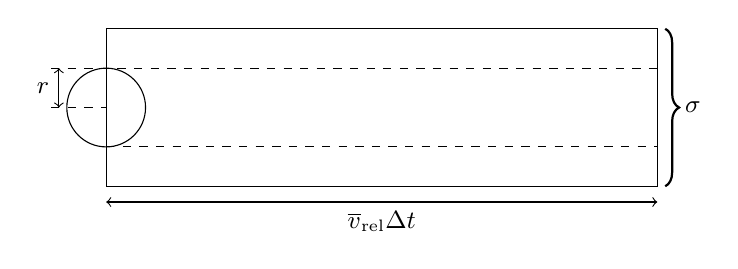
\begin{tikzpicture}
            \draw (0,0) circle (0.5);
            \draw[dashed] (-0.7,0.5)--(7,0.5);
            \draw[dashed] (0,-0.5)--(7,-0.5);
            \draw (0,-1) rectangle (7,1);
            \draw[dashed] (-0.7,0)--(0,0);
            \draw[<->] (-0.6,0)--node[left]{\small\(r\)}(-0.6,0.5);
            \draw[<->] (0,-1.2)--node[below]{\small\(\overline{v}_{\text{rel}}\Delta t\)}(7,-1.2);
            \draw [decorate,decoration={brace,amplitude=5pt,mirror},thick] (7.1,-1) -- (7.1,1) node[midway,xshift=1em]{\small \(\sigma\)};
        \end{tikzpicture}
    \end{figure}

    By the ideal gas equation, the concentration of gas is given by
    \begin{equation}\label{ideal_gas_concentration}
        c=\frac{N}{V}=\frac{p}{k_BT}\,.
    \end{equation}
    The number of collisions occurring on a specific particle over a time interval \(\Delta t\) is
    \begin{equation}
        n_{\text{col}}=\overline{v}_{\text{rel}}\Delta t\sigma c\,,
    \end{equation}
    so the collision rate is
    \begin{equation}\label{collision_rate}
        Z=\frac{n_{\text{col}}}{\Delta t}=\overline{v}_{\text{rel}}\sigma c\,.
    \end{equation}
    The speed distribution of a particle is given by the Maxwell--Boltzmann distribution
    \begin{align}
        f(v)\d{v}&=Nv^2 \ee^{-mv^2/2k_BT}\d{v}\notag\\
        &=N'\ee^{-mv^2/2k_BT}4\pi\d{v}\,,
    \end{align}
    where we can regard \(4\pi v^2\d{v}\) as the integration metric for the whole three dimension space of velocity \(\d[3]{\vb{v}}\). Hence, the velocity probability distribution is
    \begin{equation}\label{velocity_distribution}
        \phi(\vb{v})\d[3]{\vb{v}}=N'\ee^{-m\norm{\vb{v}}^2/2k_B T}\d[3]{\vb{v}}\,,
    \end{equation}
    which is a Gaussian distribution of variance \(k_B T/m\). In fact this expression can be elegantly derived from a pure symmetry argument, even if we do not know Maxwell--Boltzmann distribution.

    The probability distribution of the relative velocity between two particles \(\vb{v}_{\text{rel}}=\vb{v}_1-\vb{v}_2\) is given by the autoconvolution of (\ref{velocity_distribution}), so it is a Gaussian with a doubled variance. Hence, the probability distribution of the relative velocity
    \begin{equation}
        \psi(\vb{v}_{\text{rel}})\d[3]{\vb{v}_{\text{rel}}}=M\ee^{-m\norm{\vb{v}_{\text{rel}}}^2/4k_B T}\d[3]{\vb{v}_{\text{rel}}}\,,
    \end{equation}
    and so the relative speed distribution is
    \begin{equation}
        g(v_{\text{rel}})=M'v^2\ee^{-mv_{\text{rel}}^2/4k_B T}\d{v_{\text{rel}}}\,,
    \end{equation}
    where we can get the normalisation constant
    \begin{equation}
        M'=\frac{1}{2\sqrt{\pi}}\left(\frac{m}{k_B T}\right)^{\frac{3}{2}}
    \end{equation}
    by evaluating the integral. The average relative speed is therefore
    \begin{align}
        \overline{v}_{\text{rel}}&=\int_{0}^{\infty}\dd{v_{\text{rel}}}vg(v_{\text{rel}})\notag\\
        &=4\sqrt{\frac{k_B T}{\pi m}}\,.\label{relative_speed}
    \end{align}

    Then, we can substitute (\ref{relative_speed}) and (\ref{ideal_gas_concentration}) into the collision rate expression (\ref{collision_rate}) to get
    \begin{align}
        Z&=\sigma\left(\frac{p}{k_B T}\right)\left(\frac{16k_B T}{\pi m}\right)^{\frac{1}{2}}\notag\\
        &=\frac{4p\sigma}{\sqrt{k_B T\pi m}}\,.
    \end{align}
    Hence, the pressure broadening is given by
    \begin{align}
        \Delta \nu_{\text{press}}&=\frac{1}{2\pi\tau}=\frac{Z}{2\pi}\notag\\
        &=\frac{2\sigma}{\sqrt{k_B T\pi^3 m}}p\,.
    \end{align}

    \section{Microwave Spectra Intensities}\label{Chap:microwave_intensity}
    Consider the allowed transitions between levels \(J\) and \(J+1\), with populations \(n_J\) and \(n_{J+1}\), respectively. Note that the degeneracy of the lower level is \(2J+1\) and of the upper level is \(2J+3\). Then the net rate of absorption of photons is given by
    \begin{equation}
        \dv{n_J}{t}=-B_{J,J+1}\rho(\nu_J)n_J+B_{J+1,J}\rho(\nu_J)n_{J+1}\,.
    \end{equation}
    The first term is the stimulated absorption and the second term is the stimulated emission. We ignored the spontaneous emission because it is insignificant in the microwave regime.

    Note that the Einstein \(B\) coefficients are not the same for both processes due to degeneracies. As we stated before, the relationship is
    \begin{equation}
        \frac{B_{ij}}{B_{ji}}=\frac{g_j}{g_i}\,,
    \end{equation}
    and so we have
    \begin{equation}
        B_{J+1,J}=\frac{2J+1}{2J+3}B_{J,J+1}\,.
    \end{equation}
    The populations are given by the Boltzmann distribution
    \begin{align}
        n_J&=(2J+1)\frac{N}{q}\exp\left(-\frac{\epsilon_J}{k_B T}\right)\\
        n_{J+1}&=(2J+3)\frac{N}{q}\exp\left(-\frac{\epsilon_{J+1}}{k_B T}\right)\,.
    \end{align}
    The ratio is
    \begin{equation}
        n_{J+1}=n_J\frac{2J+3}{2J+1}\exp\left(-\frac{h\nu_J}{k_B T}\right)\,,
    \end{equation}
    where \(\nu_J\) is the frequency of the corresponding transition.

    Substituting everything into the rate expression, we get
    \begin{equation}
        \dv{n_J}{t}=-B_{J,J+1}\rho(\nu_J)n_J\left[1-\exp\left(-\frac{h\nu_J}{k_B T}\right)\right]\,.
    \end{equation}
    For rotational transitions, \(h\nu_J\ll k_B T\), so we may use Taylor expansion to obtain
    \begin{align}
        \dv{n_J}{t}&=-B_{J,J+1}\rho(\nu_J)n_J\frac{h\nu_J}{k_B T}\notag\\
        &=-B_{J,J+1}\rho(\nu_J)(2J+1)\frac{N}{q}\exp\left(-\frac{\epsilon_J}{k_B T}\right)\frac{h\nu_J}{k_B T}\,.
    \end{align}
    The rate is negative, meaning that overall stimulated absorption is faster than stimulated emission.

    Detailed calculations show that the Einstein coefficients depend on rotational levels according to
    \begin{equation}
        B_{J,J+1}=\frac{J+1}{2J+1}\,.
    \end{equation}

    Finally, note that what the spectrometer measures is the rate of absorption (or emission) of energy (that is the power). Each time the population changes by one, a photon of energy \(h\nu_J\) is absorbed (or emitted). So, the rate of absorption of energy, \(I\) is given by
    \begin{align}
        I&=\dv{n_J}{t}h\nu_J\notag\\
        &\propto(J+1)\rho(\nu_J)\nu_J^2\exp\left(-\frac{\epsilon_J}{k_B T}\right)\,.
    \end{align}
    If we assume the energy density of photons is constant, then we obtain the final result
    \begin{equation}
        I\propto(J+1)\nu_J^2\exp\left(-\frac{\epsilon_J}{k_B T}\right)\,.
    \end{equation}
    
    \section{Symmetries of Degenerate Normal Modes}\label{Chap:symmetry_degenerate_mode}
    Consider a hypothetical centrosymmetric linear molecule \(\mathrm{A-A-A}\). The bending mode is doubly degenerate: in one mode all molecules move in the \(x\) direction, and in the other mode all the molecules are moving in the \(y\) direction. They are given normal coordinates \(Q_x(x_1,x_2,x_3)\) and \(Q_y(y_1,y_2,y_3)\) respectively.

    The ground state wavefunction of this degenerate normal mode is
    \begin{equation}
        \psi_{00}=\exp\left(-\frac{1}{2}Q_x^2\right)\exp\left(-\frac{1}{2}Q_y^2\right)\,.
    \end{equation}
    The symmetry operations cause the mixing of the coordinates \(Q_x\) and \(Q_y\), so the two parts of the wavefunctions cannot be considered separately.

    We want to figure out the irreducible representation of the ground state wavefunction. For example, consider the rotation by \(\phi\) about the \(z\)-axis. This results in the mixing of the coordinates
    \begin{equation}
        \begin{pmatrix}
            x_i \\ y_i
        \end{pmatrix}\longmapsto\begin{pmatrix}
            \cos\phi & \sin\phi \\
            -\sin\phi & \cos\phi
        \end{pmatrix}\begin{pmatrix}
            x_i \\ y_i
        \end{pmatrix}\,.
    \end{equation}
    Hence we have
    \begin{equation}
        \begin{pmatrix}
            Q_x \\ Q_y
        \end{pmatrix}\longmapsto\begin{pmatrix}
            \cos\phi & \sin\phi \\
            -\sin\phi & \cos\phi
        \end{pmatrix}\begin{pmatrix}
            Q_x \\ Q_y
        \end{pmatrix}\,.
    \end{equation}
    Hence the effect of this rotation on \(\psi_{00}\) is
    \begin{align}
        &\quad \exp\left(-\frac{1}{2}Q_x^2\right)\exp\left(-\frac{1}{2}Q_y^2\right)\notag\\
        &\mapsto \exp\left(-\frac{1}{2}[Q_x \cos\phi+Q_y \sin\phi]^2\right)\exp\left(-\frac{1}{2}[-Q_x\sin\phi+ Q_y \cos\phi]^2\right)\notag\\
        &=\exp\left(-\frac{1}{2}\left[Q_x^2\cos^2\phi+2Q_xQ_y\sin\phi\cos\phi+ Q_y^2 \sin^2\phi\right]\right)\notag\\
        &\quad\times \exp\left(-\frac{1}{2}\left[Q_x^2\sin^2\phi-2Q_xQ_y\sin\phi\cos\phi+Q_y^2\cos^2\phi\right]\right)\notag\\
        &=\exp\left(-\frac{1}{2}\left[(\sin^2\phi+\cos^2\phi)Q_x^2+(\sin^2\phi+\cos^2\phi)Q_y^2\right]\right)\notag\\
        &=\exp\left(-\frac{1}{2}Q_x^2\right)\exp\left(-\frac{1}{2}Q_y^2\right)\,.
    \end{align}
    The net result is that \(\psi_{00}\) is invariant to the rotation: the same turns out to be true for any symmetry operation of the molecule. It follows that the ground state wavefunction transforms as the totally symmetric IR, \(\Sigma^+\), which is the same behaviour we have seen for non-degenerate normal modes.

    The first excited state has one quantum of excitation which can be in the mode with normal coordinate \(Q_x\), giving the wavefunction
    \begin{equation}
        \psi_{10}=\underbrace{2Q_x\exp\left(-\frac{1}{2}Q_x^2\right)}_{v_x=1}\times\underbrace{\exp\left(-\frac{1}{2}Q_y^2\right)}_{v_y=0}\,.
    \end{equation}
    Alternatively, the quantum of excitation can be in the mode with normal coordinate \(Q_y\), giving the wavefunction
    \begin{equation}
        \psi_{01}=\underbrace{\exp\left(-\frac{1}{2}Q_x^2\right)}_{v_x=0}\times\underbrace{2Q_y\exp\left(-\frac{1}{2}Q_y^2\right)}_{v_y=1}\,.
    \end{equation}
    These two wavefunctions correspond to degenerate states.

    As before, let us consider the effect of a rotation by angle \(\phi\) about \(z\) on \(\psi_{10}\) and \(\psi_{01}\). By simple algebra, we obtain
    \begin{equation}
        \begin{pmatrix}
            \psi_{01} \\ \psi_{10}
        \end{pmatrix}\longmapsto\begin{pmatrix}
            \cos\phi & \sin\phi \\
            -\sin\phi & \cos\phi
        \end{pmatrix}\begin{pmatrix}
            \psi_{01} \\ \psi_{10}
        \end{pmatrix}\,.
    \end{equation} 
    Thus \(\psi_{10}\) and \(\psi_{01}\) transform together in the same way as the normal coordinates \(Q_x\) and \(Q_y\). In other words they transform as the same IR as the normal mode, which is identical to the result we found for non-degenerate normal modes. This pair of degenerate normal modes has IR \(\Pi\), and this is consistent with the mixing going as \(\cos\phi\) and \(\sin\phi\): for the IR \(\Pi\) the character under the operation \(C_z(\alpha)\) is \(2\cos\alpha\).

    For the second excited state there are three possibilities of excitation
    \begin{alignat}{6}
        \psi_{20} &=& (4Q_x^2-2) &\exp\left(-\frac{1}{2}Q_x^2\right)\times&&\exp\left(-\frac{1}{2}Q_y^2\right)\,,\\
        \psi_{11} &=& 2Q_x &\exp\left(-\frac{1}{2}Q_x^2\right)\times&2Q_y&\exp\left(-\frac{1}{2}Q_y^2\right)\,,\\
        \psi_{02} &=& &\exp\left(-\frac{1}{2}Q_x^2\right)\times&(4Q_y^2-2)&\exp\left(-\frac{1}{2}Q_y^2\right)\,.
    \end{alignat}
    We know that the product of the exponential terms is invariant to rotations about \(z\) so we can simply ignore these terms in what follows. For reasons that will become apparent it is easier to consider the linear combinations (omitting the exponential terms)
    \begin{align}
        \psi_2'&=\frac{1}{2}(\psi_{20}+\psi_{02})=2(Q_x^2+Q_y^2)-2\\
        \psi_2''&=\frac{1}{2}(\psi_{20}-\psi_{02})=2(Q_x^2-Q_y^2)
    \end{align}
    Some straightforward but tedious algebra shows that under a rotation by \(\phi\) about the \(z\)-axis \(\psi_2'\) is invariant whereas \(\psi_2''\) and \(\psi_{11}\) are mixed, with coefficients going as \(\cos 2\phi\) and \(\sin 2\phi\).

    The invariant wavefunction transforms as one of the \(\Sigma\) IRs, because this invariance under a \(z\) rotation is a property of the \(\Sigma\) IR. To work out if the IR is \(\Sigma^+\) or \(\Sigma^-\) consider the effect of a reflection in \(xz\) plane: the coordinate \(Q_x\) is unaffected, but \(Q_y\) changes sign. However, \(\psi_2'\) depends only on the squares of these coordinates, so it is invariant to the reflection. The IR must therefore be \(\Sigma^+\).

    The two wavefunctions that are mixed must correspond to a two-dimensional \(\Delta\) IR because this IR has character \(2\cos 2\alpha\) under the operation \(C_z(\alpha)\). In summary, the second excited state of this doubly-degenerate normal mode has three degenerate wavefunctions which transform as a \(\Sigma^+\) IR and as a \(\Delta\) IR.

    This is all very well, but it is a rather laborious process. Luckily, it can be sidestepped by using a modified version of the argument we used to find the IR of the second excited-state wavefunction for a non-degenerate mode: we simply compute the direct product \(\Gamma^{(i)}\otimes\Gamma^{(i)}\), where \(\Gamma^{(i)}\) is the IR of the normal mode. Applying this approach for a \(\Pi\) degenerate mode gives the following direct product
    \begin{equation}
        \Pi\otimes\Pi=\Sigma^+\oplus[\Sigma^-]\oplus\Delta
    \end{equation}
    The difficulty is that the direct product of two two-dimensional IRs necessarily gives a result which has a total dimensionality of four --- but we only have three wavefunctions to classify. The resolution of this problem is to understand that the square bracket around \(\Sigma^-\) indicates that this IR corresponds to the antisymmetrised direct product whereas the other IRs correspond to the symmetrised direct product. For vibrational states only the symmetrised direct product is appropriate, so the \(\Sigma^-\) is rejected leaving just \(\Sigma^+\oplus\Delta\). We have already identified these as the IRs spanned by the second excited state. The method by which the IRs resulting from a direct product are classified as being from the symmetrised or antisymmetrised product is described in the course \textit{B8: Symmetry}.
    
\end{document}